\documentclass[format=draft,degree=master,language=chinese]{hustthesis}
\usepackage{algorithmic}
\usepackage{float}
%\usepackage{ctexcap}

%% 重定义章编号样式
%\CTEXsetup[number={\arabic{chapter}}]{chapter}

\stuno{M201572702}
\schoolcode{10487}
\title{基于全闪存盘阵的数据安全删除研究}{Research of Secure Deletion based on
  Solid-State Disk Array}
\author{徐德传}{Dechuan Xu}
\major{计算机技术}{Computer Technology}
\supervisor{曾令仿$\hspace{1em}$副教授}{A/Prof. Lingfang Zeng}
\date{2017}{5}{27}

\zhabstract{
    全闪存盘阵是一种全新的存储架构,由于其读写性能优越,I/O时延小,是用于取代目前阵列使用的机械硬盘的首选,
将会是未来数据中心的主流物理存储设备。但由于闪存盘硬件的特性,其上存储的数据在被删除后,数据依然存在其物理页上
,有可能造成数据泄露。基于全闪存盘阵的数据安全删除是存储研究领域积极研究的课题之一,但目前尚无很好的解决方案。


    针对固态盘的异地更新导致数据可能泄露的问题,本研究在全闪存盘阵列的基础上,提出一种通用性的方案,根据原始数据
分块后,数据块和其哈希信息等元数据经过非对称加密,产生的加密数据块再经过RS纠删码冗余编码,产生冗余加密数据单元。在擦除单个盘上的元数据,或者是
擦除一定数量的冗余加密数据块后,其对应的原始数据再也无法恢复出来,从而保证数据的安全。


    在依据研究方案实现的仿真实验上,通过对仿真系统的安全删除等功能的验证,以及对系统的数据处理带宽、I/O时延、
系统负载、数据冗余率等方面的详细测试, 结果表明,在擦除了哈希信息等元数据后,原始数据无法恢复,达到了安
全删除的目的;系统的数据处理等性能表现正常,满足可靠性和可用性的要求。}
  %%删除原始哈希信息后,保证原始数据的安全性的方案.
  %本文主要提出了一种针对全闪存盘的安全删除方法,通过对原始数据及其哈希信息在群域矩阵非对称加密运算后,
%据,在物理意义上擦除原始数据哈希信息,也即是密钥数据,达到数据安全的目的。}
\zhkeywords{固态盘,阵列,安全删除}

\enabstract{All-flash disk array is a new storage architecture. Because of its superior read and
write performance, smaller I/O latency, is preferred to be used to replace the current array that
use the mechanical hard drive. SSD will be the mainstream physical storage device used in data center
in the future. But due to the characteristics of flash disk hardware, after the data stored on it is deleted, 
the data is still existing on its physical page. There maybe caused data leakage. Secure Deletion based
on Solid-State Disk Array is one of the most active research topics in the storage field, but there hadn't good
solution yet.


For the out-of-place update of SSD may lead to data leakage problems, this study proposes a general solution, 
which raw data chunk and its hash information participate in asymmetric encryption, RS erasure code
redundance encoding, and so on,
generate redundant encrypted data units, after erasing the meta date like hash information on the key disk or erasing a certain
amount of encrypted data, the original data can no longer be recovered. Therefore, the proposol ensures the security
of data.


On the basis of simulation experiments that be achieved by the research, through verifying the secure deletion and
other functions. In addition, testing detailly data processing bandwidth, I/O latency, system load, data redundant
rate and other aspect, the result shows that, besides the simulation achieved the purpose of secure deletion that
the original data can not be recovered after deleting the hash information of the raw data, the system data
processing performance is normal and it meets the reliability and availability requirements.
}
\enkeywords{SSD, Disk Array, Secure Deletion}

\begin{document}

\frontmatter
\maketitle
\makeabstract
\tableofcontents
\listoffigures
\listoftables
\mainmatter

%% 正文
 %% 正文

\chapter{绪论}

\section{研究背景}
大容量、低成本、高性能的存储系统设计一直是存储领域研究的热点,而且随着大数据云存储时代的到来,人们对这样的存储系统的要求更加迫切。而传统的磁盘虽然容量大价格低,但磁盘的机械特性导致了它的性能在很大程度上已经到达极限。因此人们将希望寄托于新型的存储介质上,比如闪存存储器和相变存储器等。近年来固态硬盘已经成为固态硬盘(SSD)已经成为固态技术中的领先技术,最常见的SSD都是基于NAND Flash芯片设计的。SSD以闪存作为存储介质,具有随机读取速度快,功耗低,抗震性好等优点。因此目前广泛运用于家用和企业市场,在发展中的云存储系统中渐渐取代了传统的普通机械硬盘。


但是,目前依然存在一些问题,比如在对数据安全性要求高的场合,普通的SSD组成的阵列无法保证数据的安全。另外,由于SSD固有的特点,被删除的数据依旧可能被非法窃取,导致数据泄露等安全事故。针对这些存在的问题,本研究旨在固态盘阵列存储系统之上设计一套冗余存储方案,存储的数据经过与其哈希信息复杂运算后,生成冗余的加密数据,只要在物理意义上完全删除哈希信息或者一定量的数据块,原始数据即无法恢复,保证数据的安全。


固态盘的特性决定了,普通删除方式是根本不可能“真正”删除数据的,数据依然存在物理介质上\cite{ssd-outofplace-and-trim}。在对闪存页(page)写操作时,需要首先进行块擦除操作,因此,不能对闪存进行就地更新(in-place-update)的操作,只能采用异地更新(out-of-place update)的写方式,这就导致了旧的数据在某个时间窗口内依然存留在闪存上,删除操作只是系统反馈的一个“假的”删除成功。数据删除整个过程如\autoref{fig:1}所示。
\begin{figure}
\centering
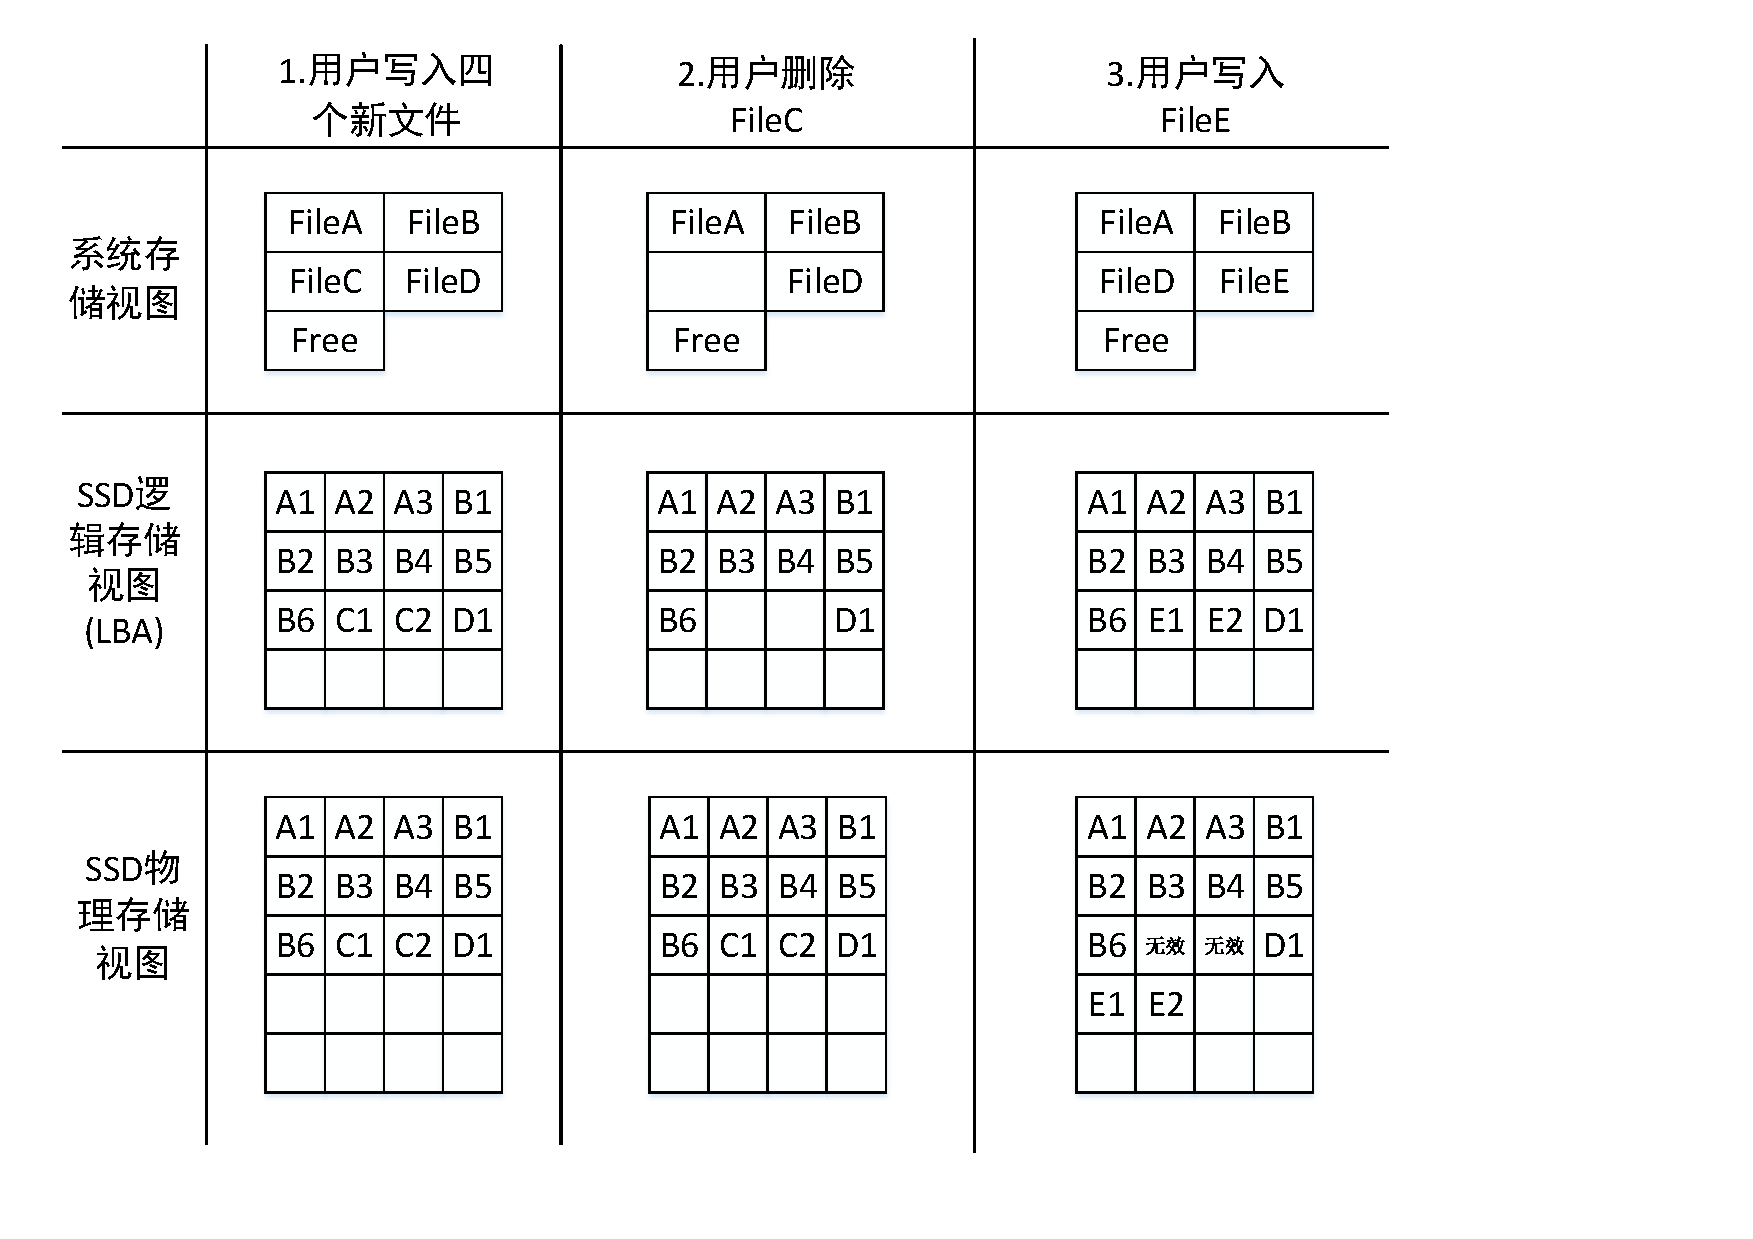
\includegraphics[width=4in]{Pics/fig-out-of-place.pdf}
\caption{固态盘异地更新}\label{fig:1}
\end{figure}
用户在文件系统上首先创建了FileA、FileB、FileC、FileD四个文件数据,反映到固态盘的逻辑块存储视图上的数据,以及在固态盘物理介质上的数据块分别如\autoref{fig:1}所示。
当用户在系统中删除了文件FileC,但是在固态盘的逻辑存储地址和物理介质上,文件C的两个数据块C1、C2却没有删除,也就是说,在用户删除文件数据的时候,数据依然存在。系统只是简单的返回一个“删除成功”的假象给用户。


第三步用户写入新的文件FileE时,虽然在固态盘逻辑块存储地址上,数据块C!,C2的位置被重新写入了新文件FileE的存储地址,但是,在固态盘物理介质上,数据块E1、E2是写入到新的位置,而旧的数据块C1、C2只是被固态盘的垃圾回收标记为“可回收”状态,真正被擦除的时机是不可控的。


从\autoref{fig:1}的三个简单操作可以发现,当用户删除了文件FileC之后,在物理介质上它的数据C1、C2在回收之前,一直都没有真正地被删除掉,这就是固态盘“异地更新”的特性,利用固态盘的这个特性,攻击者使用一些安全工具依然可以将被删掉的文件FileC恢复出来,这就造成了数据被窃取的风险。


怎样设计一套针对全闪存盘阵的安全删除方案,使得用户在物理介质上删除了元数据之后,存储的数据就能够保证安全,这就就是我们课题要研究的重点。
\section{研究目的和意义}
在信息化时代,经济、军事领域对于数据的安全性要求是比较高的。由于关键信息的泄露,可能导致国家或者个人非常重大的损失。目前,数据泄露主要存在以下三个问题:


\textbf{(1) 在数据处理、传输、存储等中间过程中,数据可能被非法复制窃取。}
例如网络传输的邮件等可能会被第三方服务商缓存下来,这种不可预知的数据复制操作在互联网时代更加普遍。导致一些企业用户纷纷兴建私有的数据中心,而不是接受公有云的服务,就是为了规避这类问题的风险。


\textbf{(2) 由于不同存储介质的特性不同,导致用户很难真正地删除数据。}虽然针对磁盘已存在很多安全工具,如 O\&O SafeErase、DataWipe、BCwipe、HDDerase、SDelete、Secure Eraser 等\cite{safe-erase,secure-eraser,bcwipe} ,这些工具基本是使用特定数据对目标文件逻辑页多次写入。对于固态盘这样的新型介质, 这些安全删除工具就不起作用。不同介质的存储设备在提供存储服务时,用户很难针对不同的设备使用不同的安全删除手段清除数据,很有可能导致数据泄露。


\textbf{(3) 数据安全删除手段可能降低存储设备或系统的可靠性以及性能。}由于工艺制程的提高,固态盘的线宽发展得更小,每单元存储的数据也越来越多,擦除寿命也变得更短\cite{Yaakobi2012Characterization,Shibata2012A}。\autoref{tab:1}显示了闪存芯片从SLC发展到QLC的线宽、擦除寿命等数据。从表中可以看出,随着闪存芯片的发展,数据安全删除的次数是不断下降的,因此,对于数据安全的删除操作,会减少闪存芯片的剩余擦除次数,使其擦除寿命降低,可能会导致坏块的增多,降低其性能,擦除操作过多更有可能导致不可预期的问题出现,影响存储设备的可靠性。
\begin{table}
\centering
\caption{SLC、MLC、TLC、QLC 四种闪存芯片的特性}\label{tab:1}
    \begin{tabular}{|*{5}{c|}}
\hline
    \multirow{2}{*}{闪存特性} & SLC & MLC & TLC & QLC \\
    & (Single-Level Cell) & (Multi-Level Cell) & (Triple-Level Cell) & (Quad-Level Cell) \\
\hline
    \textbf{存储单元模型} & 每单元一位数据 & 每单元两位数据 & 每单元三位数据 & 每单元四位数据 \\
\hline
    \textbf{速度} & 特别快 & 快 & 慢 & 很慢 \\
\hline
    \multirow{6}{*}{\textbf{擦除寿命}} & 10 万次 & 1万次 & 2500次 & 约500次 \\ %\multirow{2}{*}{约500次} \\
        & (5×nm) & (5×nm) & (5×nm) & \\ \cline{2-5}
    & 10 万次 & 5000次 & 1250次 & N/A \\%\multirow{2}{*}{N/A}  \\
        & (3×nm) & (3×nm) & (3×nm) &\\ \cline{2-5}
    & N/A & 3000次 & 750次 & N/A \\ %\multirow{2}{*}{N/A} \\
        & (2×nm) & (2×nm) & (2×nm) & \\ \hline
\end{tabular}
\end{table}


上述的三个问题说明了,一方面,数据的安全性需要做到安全删除,另一方面,研究基于固态盘阵的数据安全删除是一项有意义的工作,国内外的研究工作都处于起步阶段,积极投身这个领域将会为我国的存储安全研究打开新的局面。

\section{国内外研究现状}
近几年来,针对固态盘的安全删除技术受到了广泛关注。在国内,包括华中科技大学、中南大学、武汉大学等高等院校和科研机构都开展了相关课题和理论的研究。在国外,美国的华盛顿大学、哥伦比亚大学以及IBM、HP等实验室也积极地投身在安全删除领域的研究上。
\subsection{基于密码学意义上的安全删除}
数据在被加密存储之后,如何保证删除密钥数据,原来的数据就无法再被还原,成为新的难题。Perlman等人首次提出了基于时间的数据安全删除方法,针对加密文件,如果密钥过期后数据即被删除,而且文件无法恢复\cite{Perlman2005File}。受Perlman等人的启发,Tang等人设计出了FADE系统\cite{Tang2012Secure},该系统使用公钥密码并使用简单的布尔操作来调整安全删除策略。但是FADE只支持一到两层的布尔表达,而且需要使用复杂的公钥系统。Perlman等人还设计了Ephemerizer系统\cite{Perlman2005The,Tang2009Timed},该系统需要一个可信服务器保存并管理由数据拥有者指定过期时间的解密密钥。Geambasu 等人给出了一个基于时间的数据可信删除方法的原型 Vanish\cite{Geambasu2009Vanish},但Vanish容易受到跳跃攻击(hopping attack)和嗅探攻击(sniffing attack)\cite{Wolchok2010Defeating} 。华中科技大学武汉光电国家实验室曾令仿等人提出了一种SafeVanish\cite{Zeng2010SafeVanish}方案,通过扩展密钥等份长度的方法提高跳跃攻击的成本,并且引入公钥密码体制抵御嗅探攻击,显著改善了Vanish方案。Reimann等人\cite{Reimann2012Timed}针对Vanish系统中当文件在 8 小时后需要被访问时,文件拥有者需要更新节点缓存中的密钥部分问题,提出了将密钥分量分发到随机的网页中保存的改进方案,随着时间的改变,网页会改变存储内容或是被删除。
针对以Vanish为代表的加密方案存在的单个密钥加密全部数据不能对数据进行细粒度的管理等问题,武汉大学王丽娜等人\cite{王丽娜2012一种适于云存储的数据确定性删除方法}提出了利用秘钥生成树,门限秘密共享(threshold secret sharing)来组织和管理秘钥,同时利用分布式散列表(distributed hash table,DHT)周期性地删除相关秘钥来实现安全删除。中南大学王国军等人改进了Vanish方案,除了将密钥分发到 DHT 网络中,还提取部分密文并分发到DHT 网络中,从而更有效抵抗传统密码分析和暴力攻击\cite{Wang2010A}。西安电子科技大学马建峰和中国科学院信息工程研究所李凤华所在课题组针对网络内容生命周期隐私保护问题,提出了面向网络内容隐私的基于
身份加密的安全自毁方案\cite{熊金波2014云计算环境中的组合文档模型及其访问控制方案,熊金波2014基于属性加密的组合文档安全自毁方案,熊金波2014面向网络内容隐私的基于身份加密的安全自毁方案},这种方案基于身份的加密和分布式Hash表(DHT)网络。这些方案更多的是偏向上层应用,在原型系统方面的实现和方法验证方面显得不足。针对密钥从物理介质上“真正地”删除,这些方案涉及的研究都不是很深。
\subsection{物理介质上数据安全删除}
面对这一问题,研究者有的提出了从物理损坏或者化学破坏的方式,这种方法不本方案不涉及相关研究。
M.Wei的一个研究\cite{Wei2011Reliably}表明:
\begin{enumerate}
\item 存储介质的内建命令通常能提供有效的数据擦除功能,但是并不能保证这些命令总是被制造商正确地实现
\item 将SSD的所有数据全部覆盖两次(在大部分情况下)能够有效地清除数据
\item 对于单个数据块删除而言,当前的SSD都存在不足之处
\end{enumerate}


因此,这一过程的实现并不一直是正确的,在有些情况,文件系统显示已被删除,而数据仍在设备中存在。Peterson等人\cite{Peterson2005Secure}在
数据块层使用全有或全无的转换技术(AONT)来实施安全删除,该方法通过AONT存储每一个数据块,然后覆盖其中的一部分,这使得整个数据块不可用。2012年,Diesburg提出TrueErase\cite{Diesburg2012TrueErase},一种类似于TRIM指令的功能,但是只针对属于某敏感文件的数据块。他们在文件系统和设备驱动之间增加了一个新的传输通道。被修改的设备驱动一旦接受到被删除块的信息,使用其下层的接口就可以实现快速安全删除。TrueErase比TRIM更有效,因为它可以只是安全擦除部分敏感块。TrueErase改造了存储管理层,
全方位监控敏感文件的编辑和更新,并可彻底删除敏感文件,前提是假设文件系统可以直接访问和操作物理闪存,所以其缺点是无法应用于普通固态盘。


总体来说,针对全闪存盘阵应用场景,目前研究都处在初始阶段,需要采用新的架构来保证数据的安全删除\cite{傅颖勋2013安全云存储系统与关键技术综述}。现有研究偏向
上层应用,并且越是接近上层系统越抽象,数据确定性删除就越困难\cite{Reardon2013SoK},也难以在存储性能、计算开销和数据通信延迟方面达到很好的平衡\cite{李晖2014公共云存储服务数据安全及隐私保护技术综述}。另外,现有研究缺乏从数据按需删除的角度,只针对敏感数据实施安全删除,从而并不改变普通用户的使用习惯,或根据不同的安全级别需求采取“合理”的数据安全删除策略。
\section{本文的研究内容}
本研究旨在提供一种基于闪存盘组成的阵列的数据安全删除方案。通过对数据进行冗余加密,保障数据安全存储,即高可靠性和高安全性。一方面,采用了非对称加密算法、群域运算保障数据可靠性;另一方面,在编码前引入加密的方式增强数据隐私保护,利用冗余编码的特性结合弱密钥思想,对数据的删除不再需要对整个数据进行覆盖写,而是删除部分数据块,破坏数据完整性或者密钥完整性,使数据无法正常读取。即使攻击者得到数据,也不能获取明文,达到数据安全删除的目的。本研究在保证数据安全存储的同时,降低了对固态盘阵列的读写访问,相当于延长了固态盘的使用寿命。

\chapter{方案系统设计}
\section{方案前提}
方案是将密钥数据和冗余加密后的数据分别存放在单块固态盘和固态盘阵,因此安全删除数据的关键是要完全擦除单块固态盘上的密钥数据,所以,本方案是构建在单块固态盘支持TRIM命令,并且可以安全擦除据的基础上的。
\section{技术关键}
随着原始数据量的增长,加密数据单元的大小选取将对整体的数据存储时间损耗产生显著影响。同时,加密算法的设计也需要重点关注,分散加密算法的三个关键参数(n,k,r),n表示最终生成的数据单元,。k表示恢复原始数据所需要的最低数据单元数量,r表示如果有效的加密数据单元不大于r值,则数据无法恢复。如何设计这样一个算法,完成数据的加密,同时占用的存取时间尽可能少。 
完全删除存储的密钥数据,可以利用固态盘的TRIM指令,在需要频繁安全删除数据的场合,可以显著的提升固态盘阵列的性能。传统的机械硬盘在删除数据的时候,简单的在逻辑数据表内把存储要删除的数据的位置标记为可用而已,使用机械硬盘的系统根本就不需要向存储设备发送任何有关文件删除的消息,因为在将来,系统可以随时把新数据直接覆盖到无用的数据上。使用固态盘就不同,当系统准备把新数据要写入那个位置的时候,固态硬盘才意识到原来这写数据已经被删除了。


由于固态盘支持TRIM指令,系统在删除逻辑表中删除逻辑扇区地址的同时通知固态硬盘某些数据已经无用了。TRIM的先进性在于它可以让固态硬盘在进行垃圾回收的时候跳过移动无用数据的过程,从而不再用重新写入这些无用的数据,达到节省时间的目的。同时也减少了闪存删除数据的次数,从而在写入过程中实现高性能。固态硬盘也不需要立即删除或者“垃圾回收”这些TRIM指令告知的位置了,它只是先标记这些位置的数据为“无用”即可。


支持TRIM的系统,在用户写入数据时并没有不同。但是当用户删除文件的时候,因为系统支持了TRIM指令,固态硬盘立刻就把数据标记为“无用”,从而为接下来的垃圾回收做准备。原来存放该文件的空间,固态硬盘把其看做是可用空间,这意味着固态硬盘在执行垃圾回收的过程中拥有更多的可用空间,从而整体提高性能。支持TRIM命令的固态盘更新文件如\autoref{fig:2}所示。
\begin{figure}[H]
	\centering
	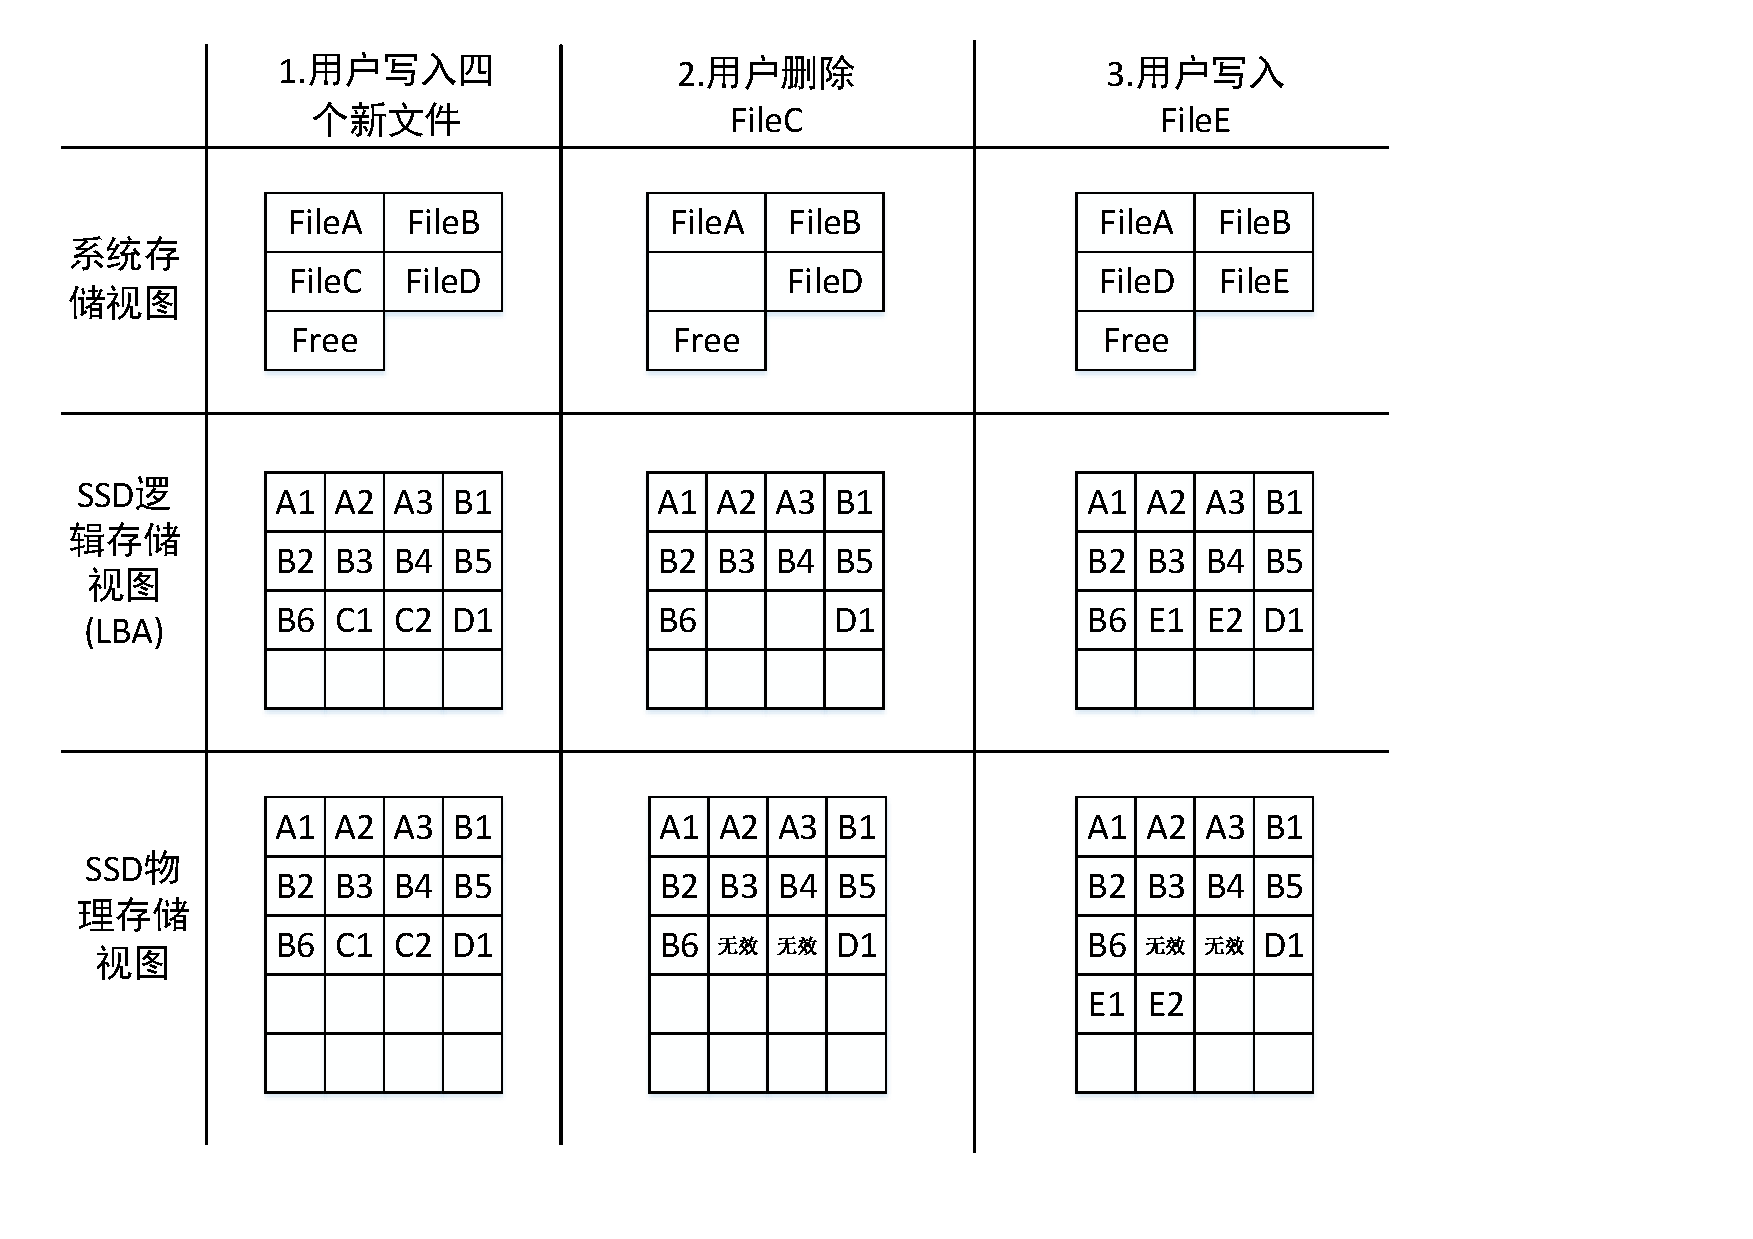
\includegraphics[width=4in]{Pics/trim.pdf}
	\caption{支持TRIM的固态盘删除、更新数据操作}\label{fig:2}
\end{figure}
在\autoref{fig:2}中的更新文件过程中,删除文件C时,删除指令立即调用內建的TRIM命令准备回收文件C占用的C1,C2两个数据块,物理介质上,这两个数据块已经被标记被“回收”状态,这样每次GC的时候就不用再移动C1、C2两个数据块,减少了数据泄露窗口和数据写入量。


如何确保原始数据不被非法地逆向解密读取出来,涉及到这套方案的冗余加密模块的两个关键参数:(1)直接参与运算的密钥数据;(2)加密后相互独立的数据块单元。只要将这两个条件中任意一个的数据“真正”地破坏掉,原始数据就再也无法恢复。


安全删除密钥数据,需要从物理意义上真正地将密钥擦除。目前,针对固态盘数据主流的物理擦除方法主要有以下三种:
\begin{itemize}
	\item 使用固态盘驱动器的ATA安全擦除。SSD固件有一个嵌入命令,可以将驱动器的每一个数据位覆写为0,从而达到安全删除数据的目的。这种擦除手段使用引导环境下的USB闪存盘,运行相应的清除工具即可以进行。
	\item 使用自加密驱动器的加密擦除。在一个自加密的固态盘驱动器(SED)上,加密密钥存储在驱动器的一块小型存储区域,由内部硬件加密待存储的数据和解密预备读取的数据,并且使用安全管理软件管理。我们可以将文件的加密密钥放置在该类SSD上,需要删除数据时。进入SED的管理软件,删除并重新生成固态盘的密钥。这将导致先前写入的密钥数据完全不可读。因此,冗余加密方案生成的数据也就无法还原成原始数据。
	\item 损坏密钥存储区的物理介质、这种擦除手段是将SSD介质通过标准的高温或者细化手段破坏,以至于不可再读。适用于安全要求非常高的应用场合。
\end{itemize}


为了适应大多数的固态盘的特性,本方案采用的是ATA安全擦除。一方面,带有自加密的固态盘厂商不一定完全设计实现,不能针对所有的固态盘硬件,并且物理或者化学方式的损坏不在方案的讨论范围;另一方面,ATA安全擦除方法操作相对简单,而且即使系统被恶意破坏,我们也可以通过引导方式下的安全擦除(Secure Erase)功能擦除密钥,保证数据的安全性。


ATA安全擦除方法根据具体固态盘厂商的实现,內建的擦除命令使用的基本是覆写数据的方法,即对固态盘的物理页覆写特定的数据多次,达到无法恢复原始数据的目的,这种覆写手段通常最高能达到95.9-99.9\%的数据完全擦除\cite{Wei2011Reliably}。


在M.Wei的论文\cite{Wei2011Reliably}中指出,验证数据安全删除需要绕过文件系统,直接读取闪存芯片的数据。需要使用特殊的读取设备Ming the Merciless如\autoref{fig:3}所示。直接连接闪存芯片的针脚,读取其中的数据,从而避免了闪存转换层(FTL)的干扰。
\begin{figure}[H]
	\centering
	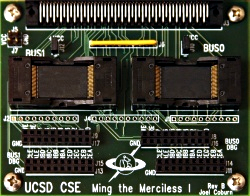
\includegraphics[width=2in]{Pics/ming.png}
	\caption{Ming the Merciless}
    \label{fig:3}
\end{figure}
针对本方案涉及到的两个关键问题:(1)数据安全删除;(2)系统可用性或者是可靠性。技术关键就是为了解决怎样安全删除的问题,系统可靠性应该依赖于在解决安全删除的基础之上进行的改进。
\section{方案详细设计}
\subsection{模块架构}
将多个SSD组成一个存储阵列。对于上层组件,如文件系统,将SSD看做一个简单的块设备,而不关心其内部的负载结构。用户可以在上面创建分区和文件系统,和普通硬盘一样。这样很容易整合到现有系统,因为对整个系统的改动很小。整体模块架构如\autoref{fig:4}所示。
\begin{figure}[H]
	\centering
	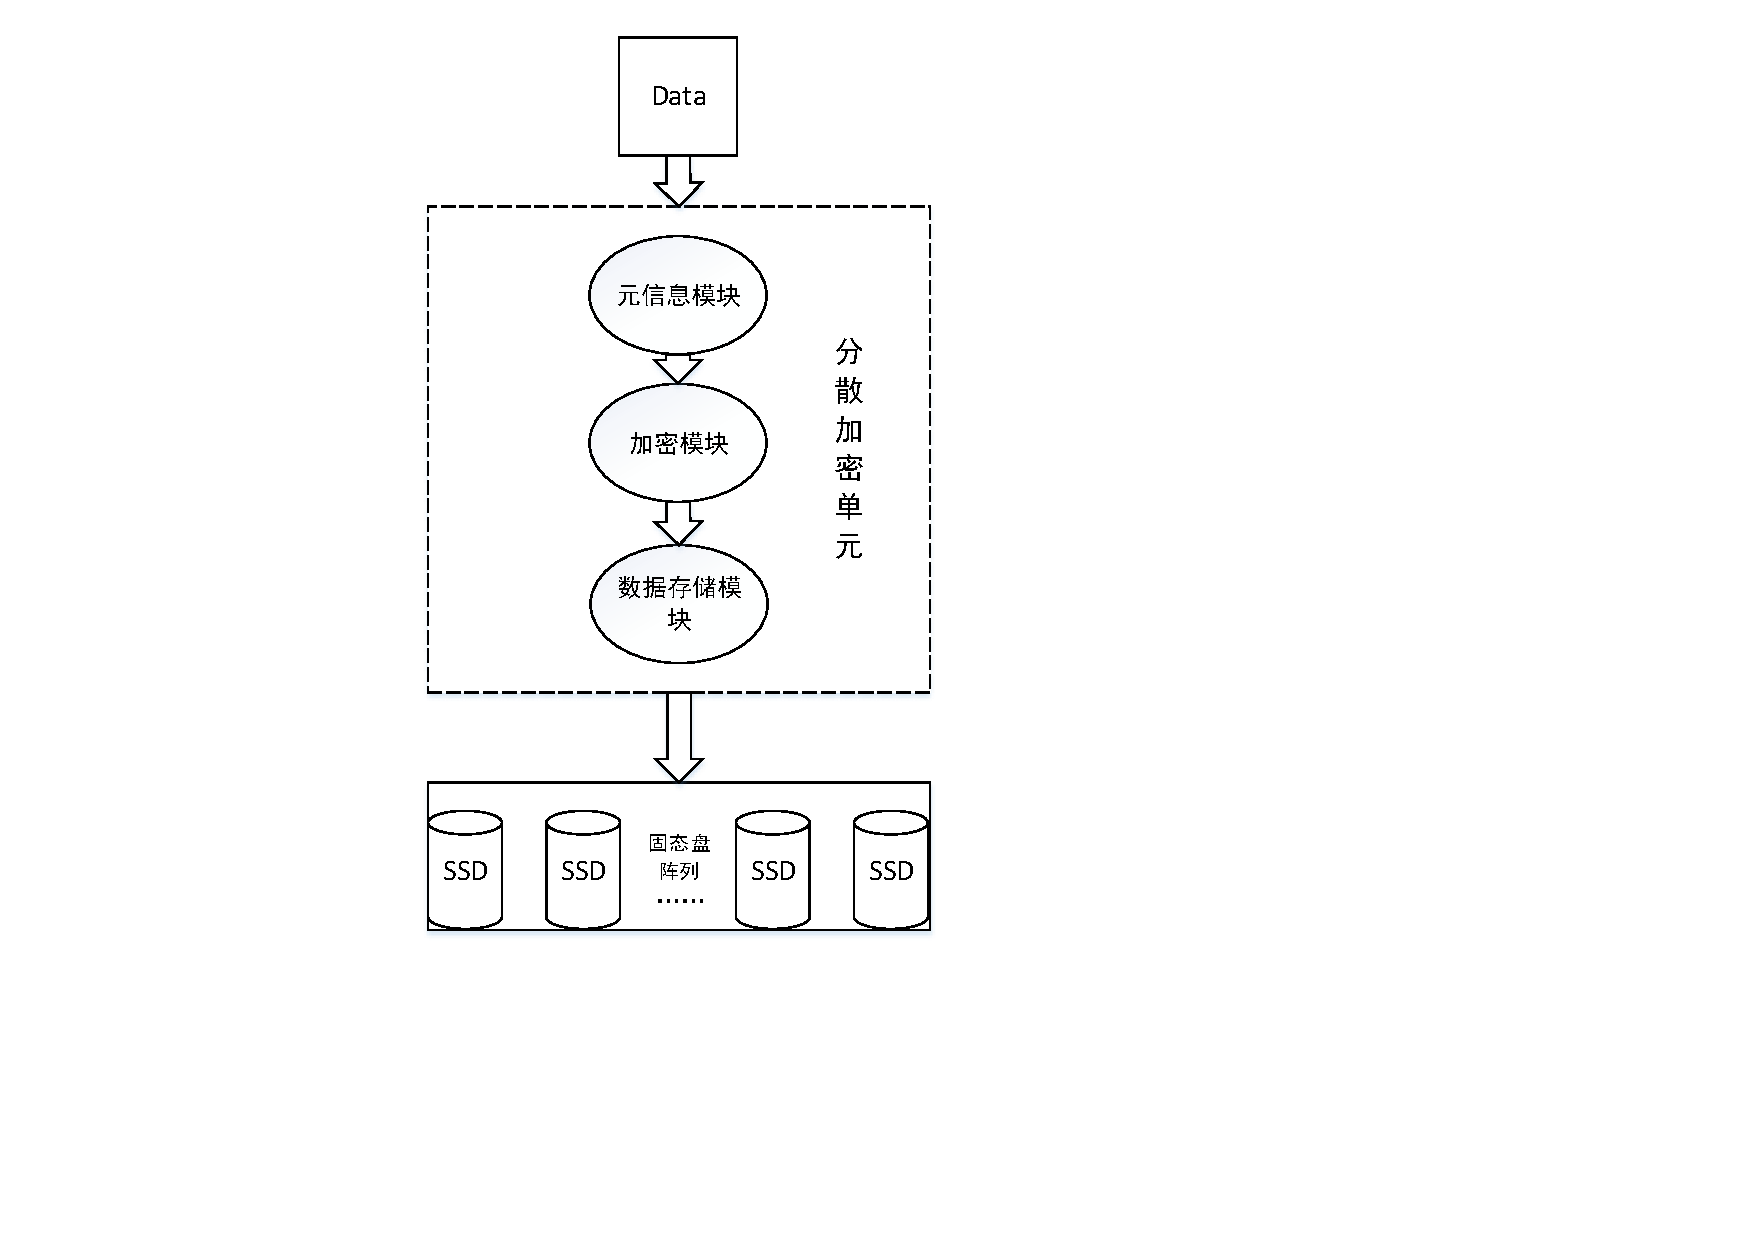
\includegraphics[width=3in]{Pics/total-structure.pdf}
    \caption{模块功能架构}
    \label{fig:4}
\end{figure}
原始数据经过分散加密系统,首先是数据分成一个个的加密单元数据块,在系统中目前选取的平均数据块大小是8k,然后由数据标记中心记录原始数据块的信息,将一定数量的原始数据输入加密模块,得到加密后的数据块,进入数据分发缓存,同时反馈存储位置信息,最后将加密数据写入阵列的相应独立区域中。
\subsection{加密算法设计}
整体加密流程如\autoref{fig:5}所示。
\begin{figure}[H]
	\centering
	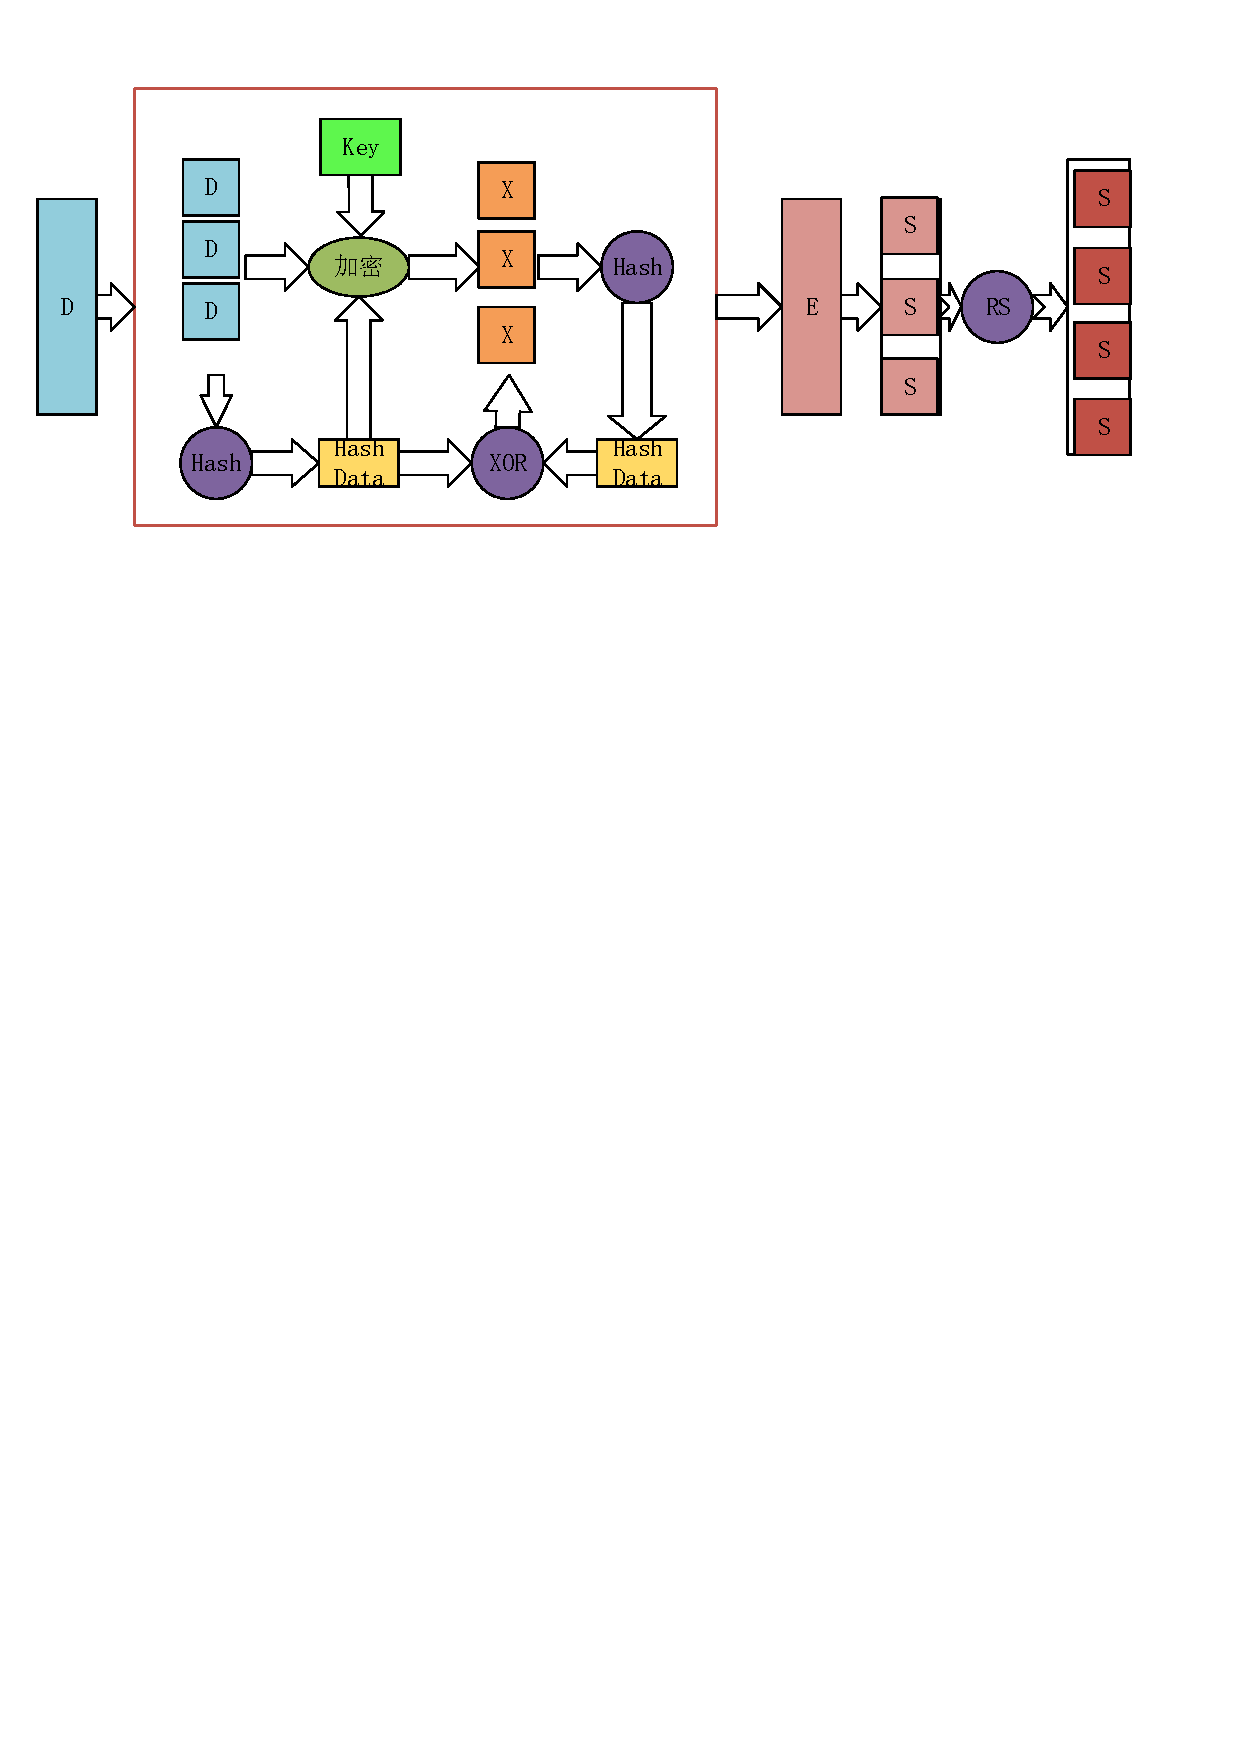
\includegraphics[width=4in]{Pics/encrypt.pdf}
	\caption{加密算法流程}\label{fig:5}
\end{figure}
加密模块在输入原始数据块后,首先分为大小一定的数据块,进行一系列的哈希运算和加密操作后,得到初始的加密数据块X,再由X的哈希信息数据和之前原始数据的哈希信息数据异或操作得到初步的加密数据块。这些数据块组合成大小相同的加密数据单元S,最后由冗余运算模块操作得到最终的加密存储数据。详细的加密流程与算法如\autoref{eq:1}所示。
\begin{equation}
    \label{eq:1}
    \begin{aligned}
        c_{i} &=d_{0} \bigoplus E(h_{key},i),i=0,1,...,s-1 \\ % 注释有特殊符号
        c_{s} &=h_{key} \bigoplus H(c_0,c_1,...,c_{s-1})     
    \end{aligned}
\end{equation}
\footnote{$\bigoplus$ 表示异或操作
\newline h$_{key}$表示对数据块取哈希操作,安全领域使用的主流哈希算法有SHA-128、SHA-256等
\newline E表示非对称加密算法,常用的算法有AES-128、AES-256
}
\footnote{}
\begin{enumerate}
    \item 将原始数据D分割成d$_{0}$,d$_{1}$,...,d$_{s-1}$共s个数据块,按照\autoref{eq:1}的运算得到初步加密后的数据块c$_{1}$ ,c$_{2}$,…,c$_{s}$
	\item 加密后的数据块经过群运算得到最终相互独立的加密数据单元
\end{enumerate}

\subsection{破坏恢复条件}
前面已经提到,为了使原始数据再不可恢复,针对加密后的数据,可以有两种解决办法:一是至少删除n-r份数据单元的加密数据,使得数据解密的条件被破坏;二是完全删除密钥区的数据,没有密钥参与解密运算,此时就无法恢复原始数据。两种删除方法分别对应\autoref{fig:6}和\autoref{fig:7}所示。
\begin{figure}[H]
	\centering
	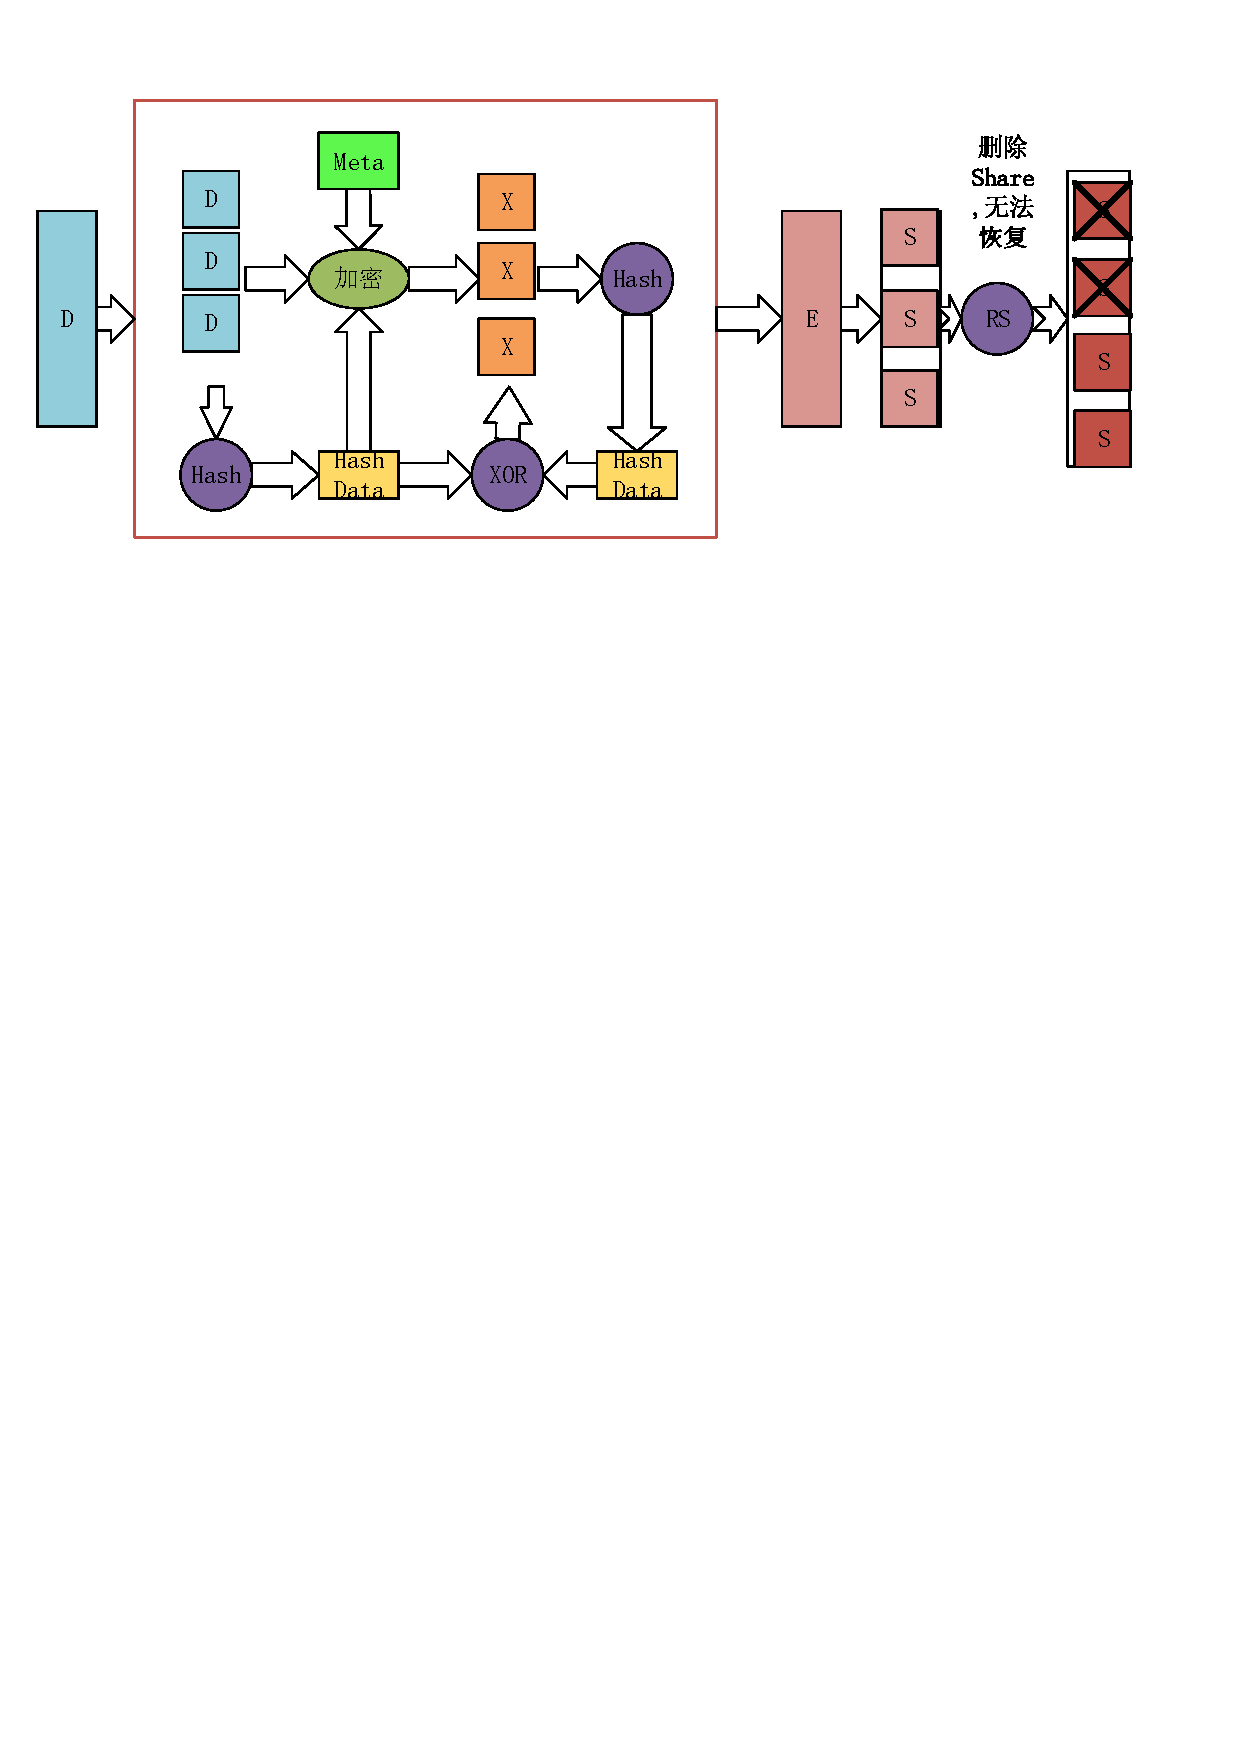
\includegraphics[width=4in]{Pics/del-share.pdf}
	\caption{删除Share的方法}\label{fig:6}
\end{figure}
\begin{figure}[H]
	\centering
	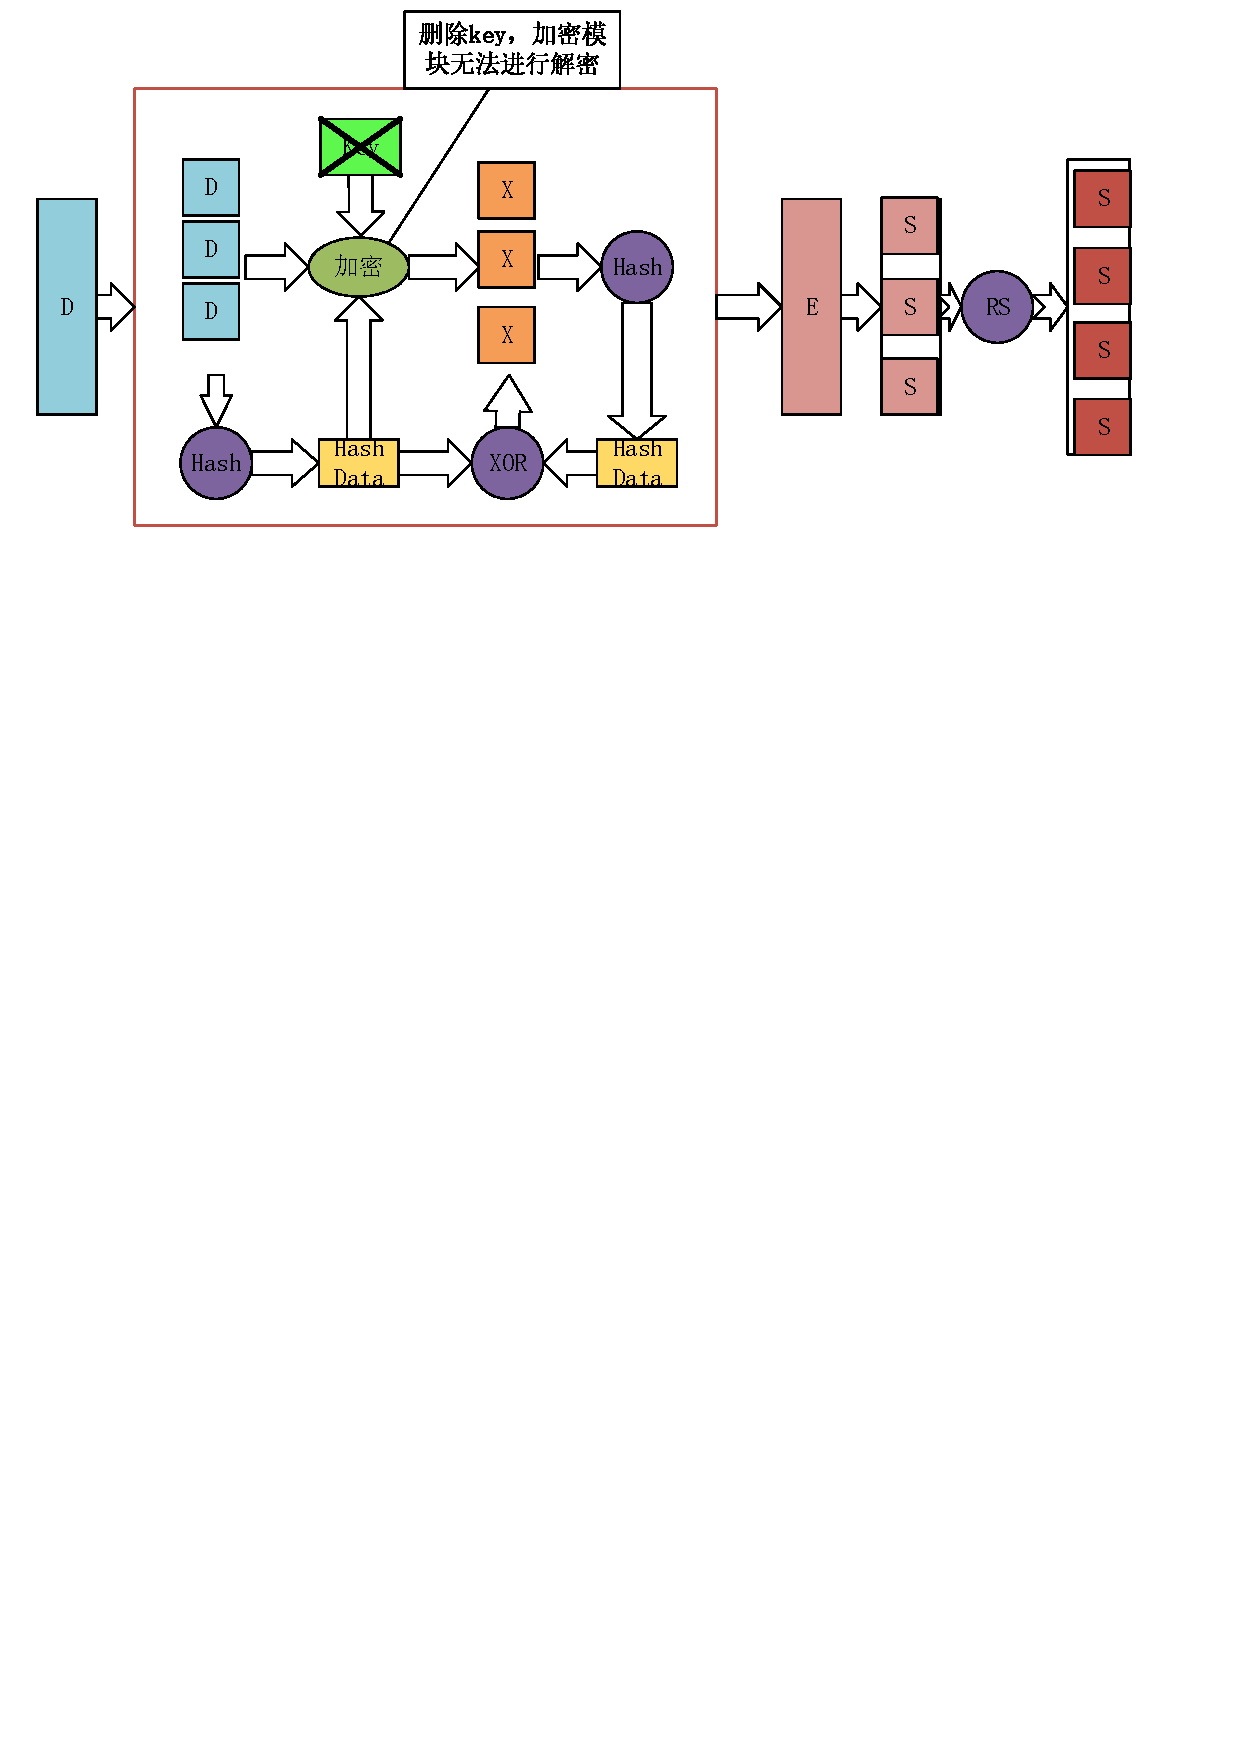
\includegraphics[width=4in]{Pics/del-hashkey.pdf}
	\caption{删除存储的哈希数据}\label{fig:7}
\end{figure}


这里我们选择的是删除哈希信息数据,有如下三个原因:
\begin{itemize}
	\item 密钥区的数据通常都比较少,而且大小固定。可以利用固态盘的特殊性,安全的删除。而删除Share数据量太大,对固态盘阵列来说,势必会降低其使用寿命。
	\item 固态盘使用TRIM指令可以很快速地完全删除,真正地达到清除的地步。而完全删除相互独立的加密数据单元是一件非常耗时的操作,会显著影响系统的可用性,在一些频繁操作的场合,这种方案的劣势会更加突出。
	\item 可以将整个加密系统采用的随机密钥数据存放在一个独立的固态盘上,需要删除时,直接使用擦除软件安全删除密钥,管理比较方便。而删除加密数据单元的手段比较费时费力,无法集中管理。
\end{itemize}

\subsection{从物理介质上删除敏感信息数据}
方案采用的是将哈希信息等密钥数据单独存储在一个固态盘上,需要删除对应的数据时。使用ATA低级擦除方法擦除该固态盘数据,即多次写入方法,首先数据位全部覆写0,然后写入随机数据,最后再次擦除数据,达到安全删除的效果\cite{Lee2008Secure,Swanson2010Safe}。
%目前,使用经过验证的Parted Magic这类软件的安全擦除法,能够确实有效地物理擦除数据。
\section{方案整体流程}
本方案采用的方案是在SSD组成的混合存储结构上,分出一个单独的密钥盘存放密钥数据,使用多个SSD组成盘阵,用来存放加密后的数据单元。整体结构如\autoref{fig:8}所示。
\begin{figure}[H]
	\centering
	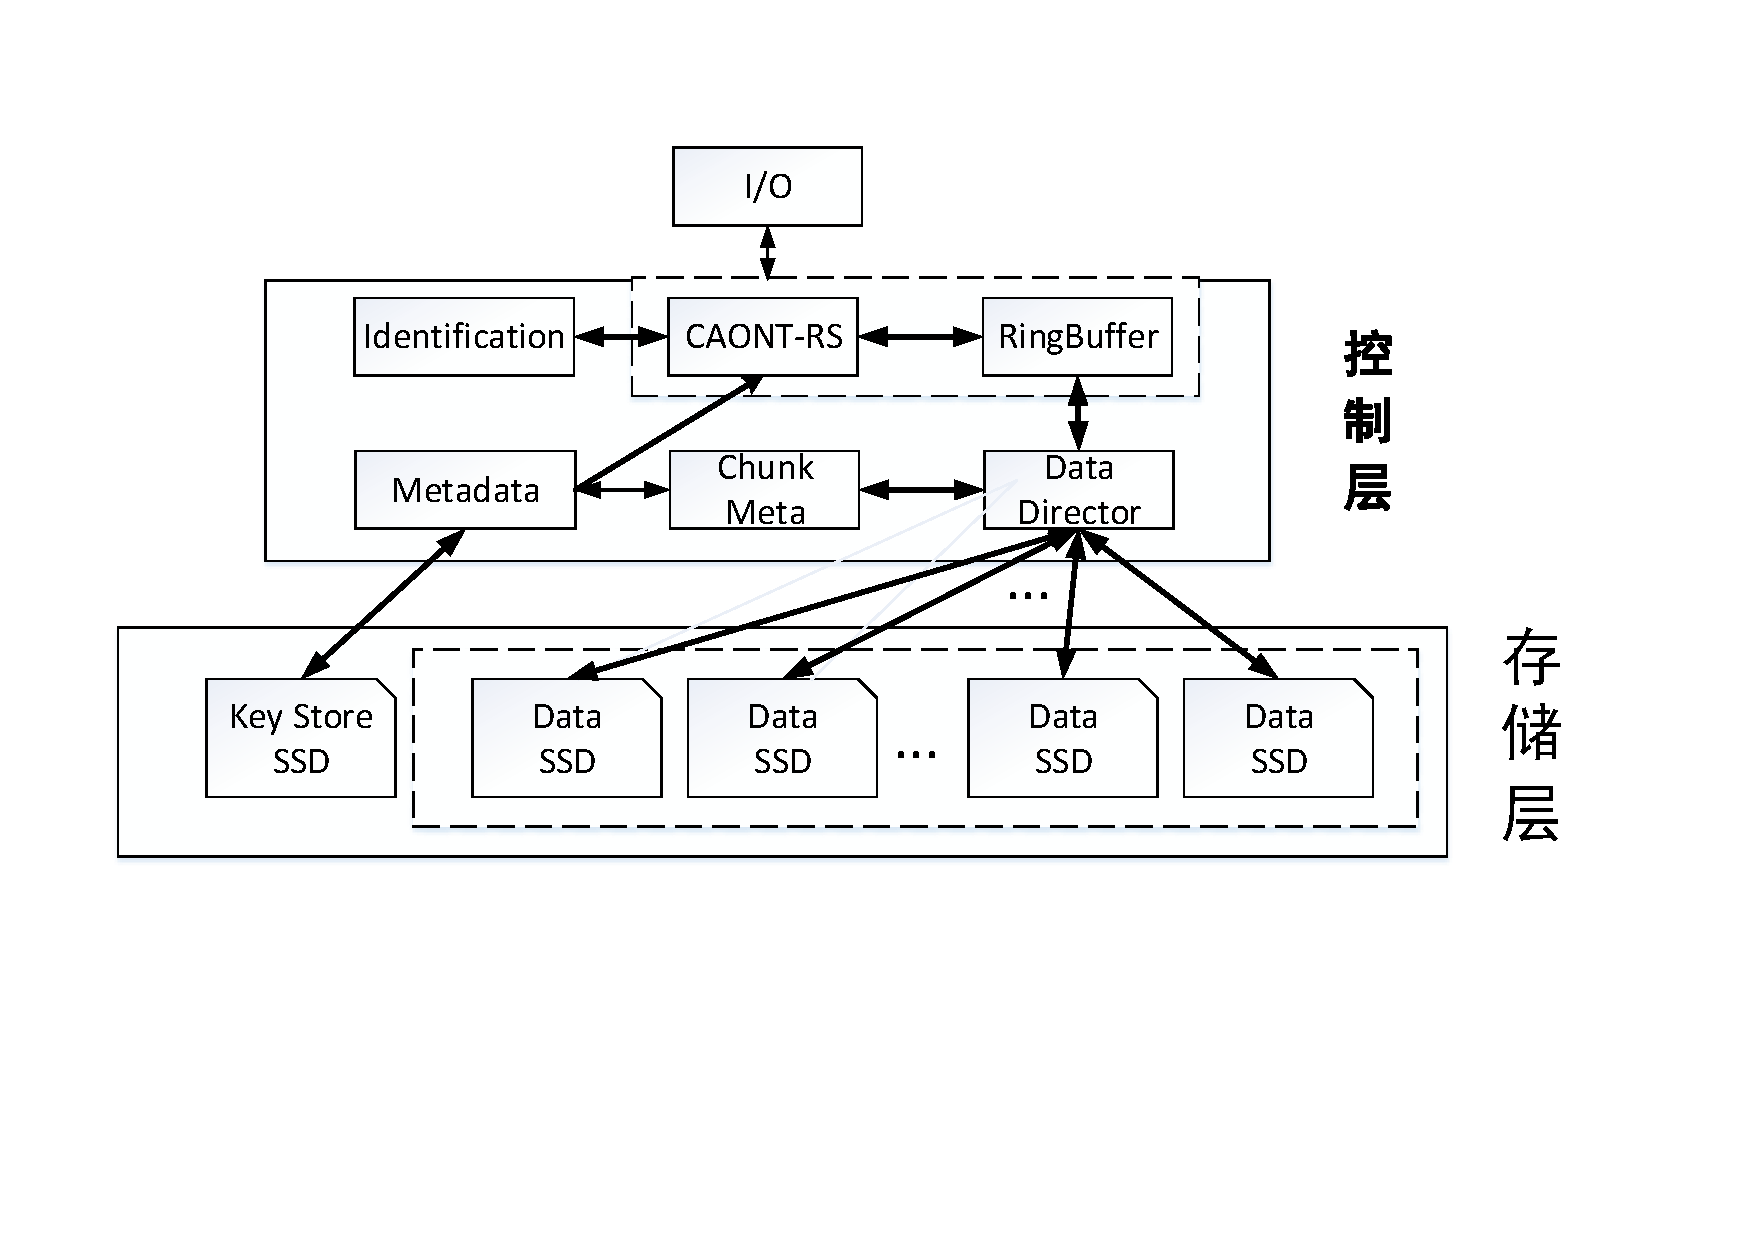
\includegraphics[width=1\textwidth]{Pics/total-store-structure.pdf}
	\caption{系统整体架构}\label{fig:8}
\end{figure}
当有I/O请求到来时,逻辑控制层首先将数据分成固定大小的数据块标识每一个数据块的序号。同时,密钥生成块产生随机32位数据作为密钥与数据块起输入冗余加密模块加密,生成冗余数据块,输出到循环队列中缓存等待存储。数据块信息注册模块录下加密后的数据块的编号,由数据分发模块将相互独立的数据单元有序分发到数据盘。与此同时,密钥数据存储在密钥盘。在安全删除部分,我们只需要将密钥盘安全擦除数据即可。\\


下面结合方案的具体功能详细描述系统读、写、删除的流程。
\subsection{系统写入数据}
\begin{figure}[H]
	\centering
	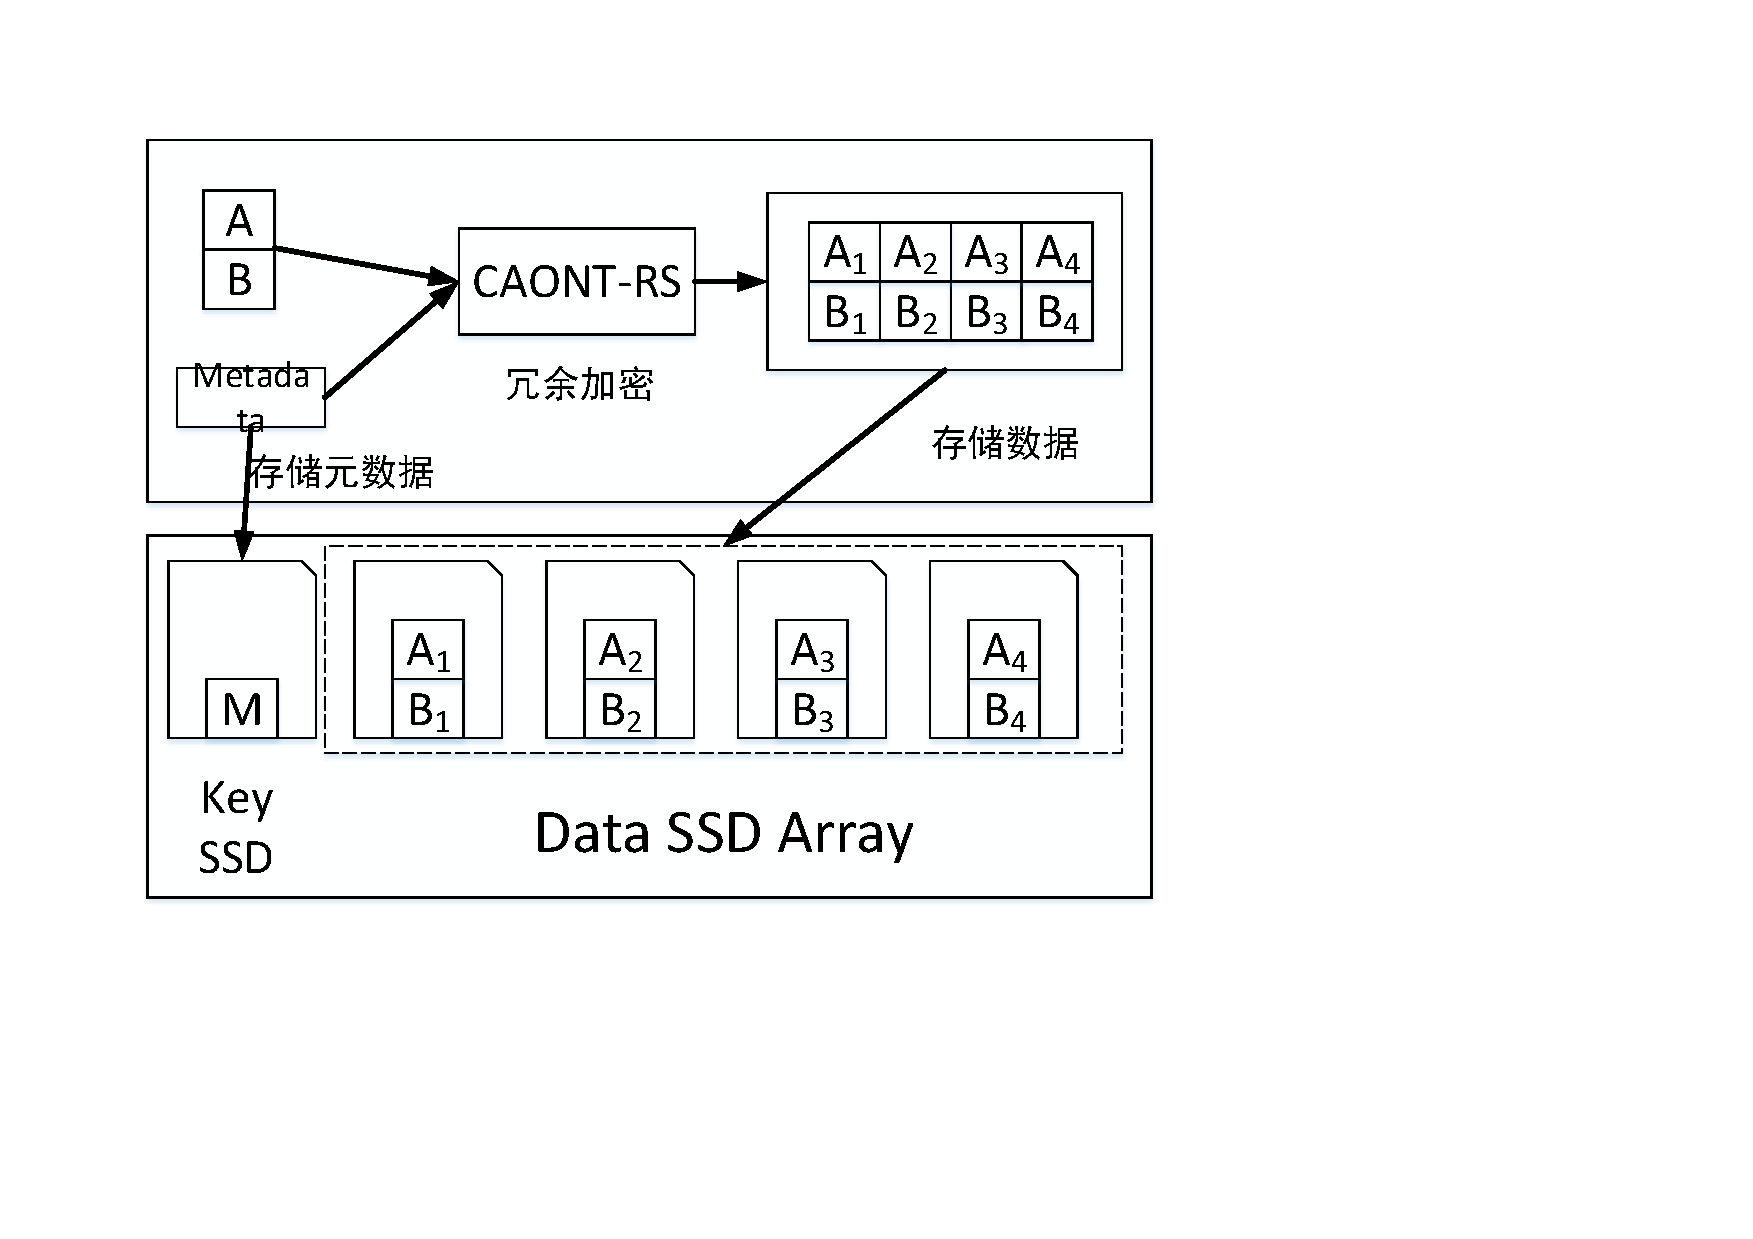
\includegraphics[width=4in]{Pics/data-write-st.pdf}
	\caption{数据写入架构}\label{fig:9}
\end{figure}
\begin{figure}[H]
	\centering
	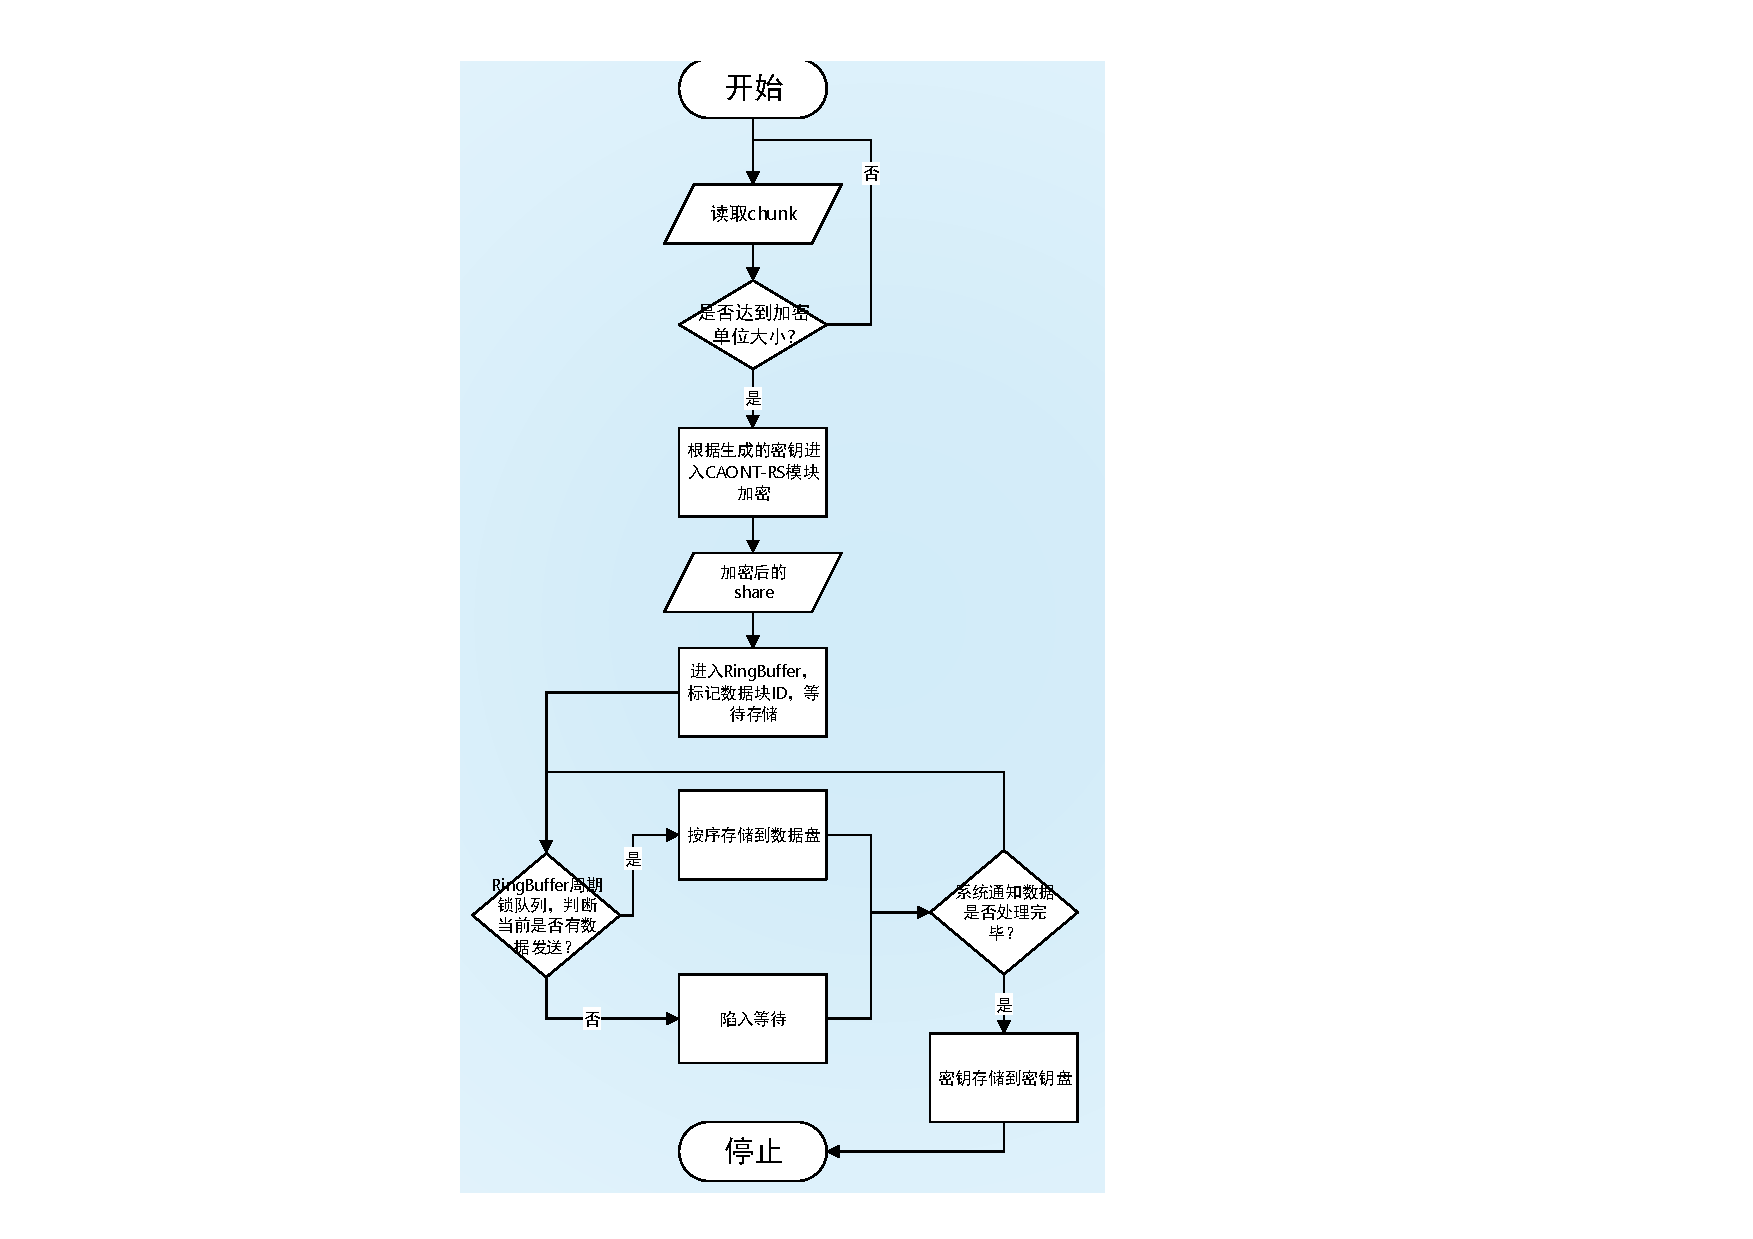
\includegraphics[width=4in]{Pics/data-write-pr.pdf}
	\caption{数据写入流程}\label{fig:10}
\end{figure}
在\autoref{fig:9}的数据写入存储结构以及\autoref{fig:10}数据写入流程中,当系统写入文件时,加密模块首先判断数据是否达到加密单元的大小,并且这个数据粒度可以调整。与此同时,密钥模块随机产生密钥数据,一起输入到加密模块,产生冗余的加密数据单元,并且按照顺序缓存到循环队列中等待存储,循环队列周期性地检查是否有数据需要转发存储,将数据依据数据盘的数量依次轮询发送存储请求。数据处理完毕,密钥模块将密钥数据存放到密钥盘,整个系统的加密写入流程完成。
\subsection{系统读取数据}
\begin{figure}[H]
	\centering
	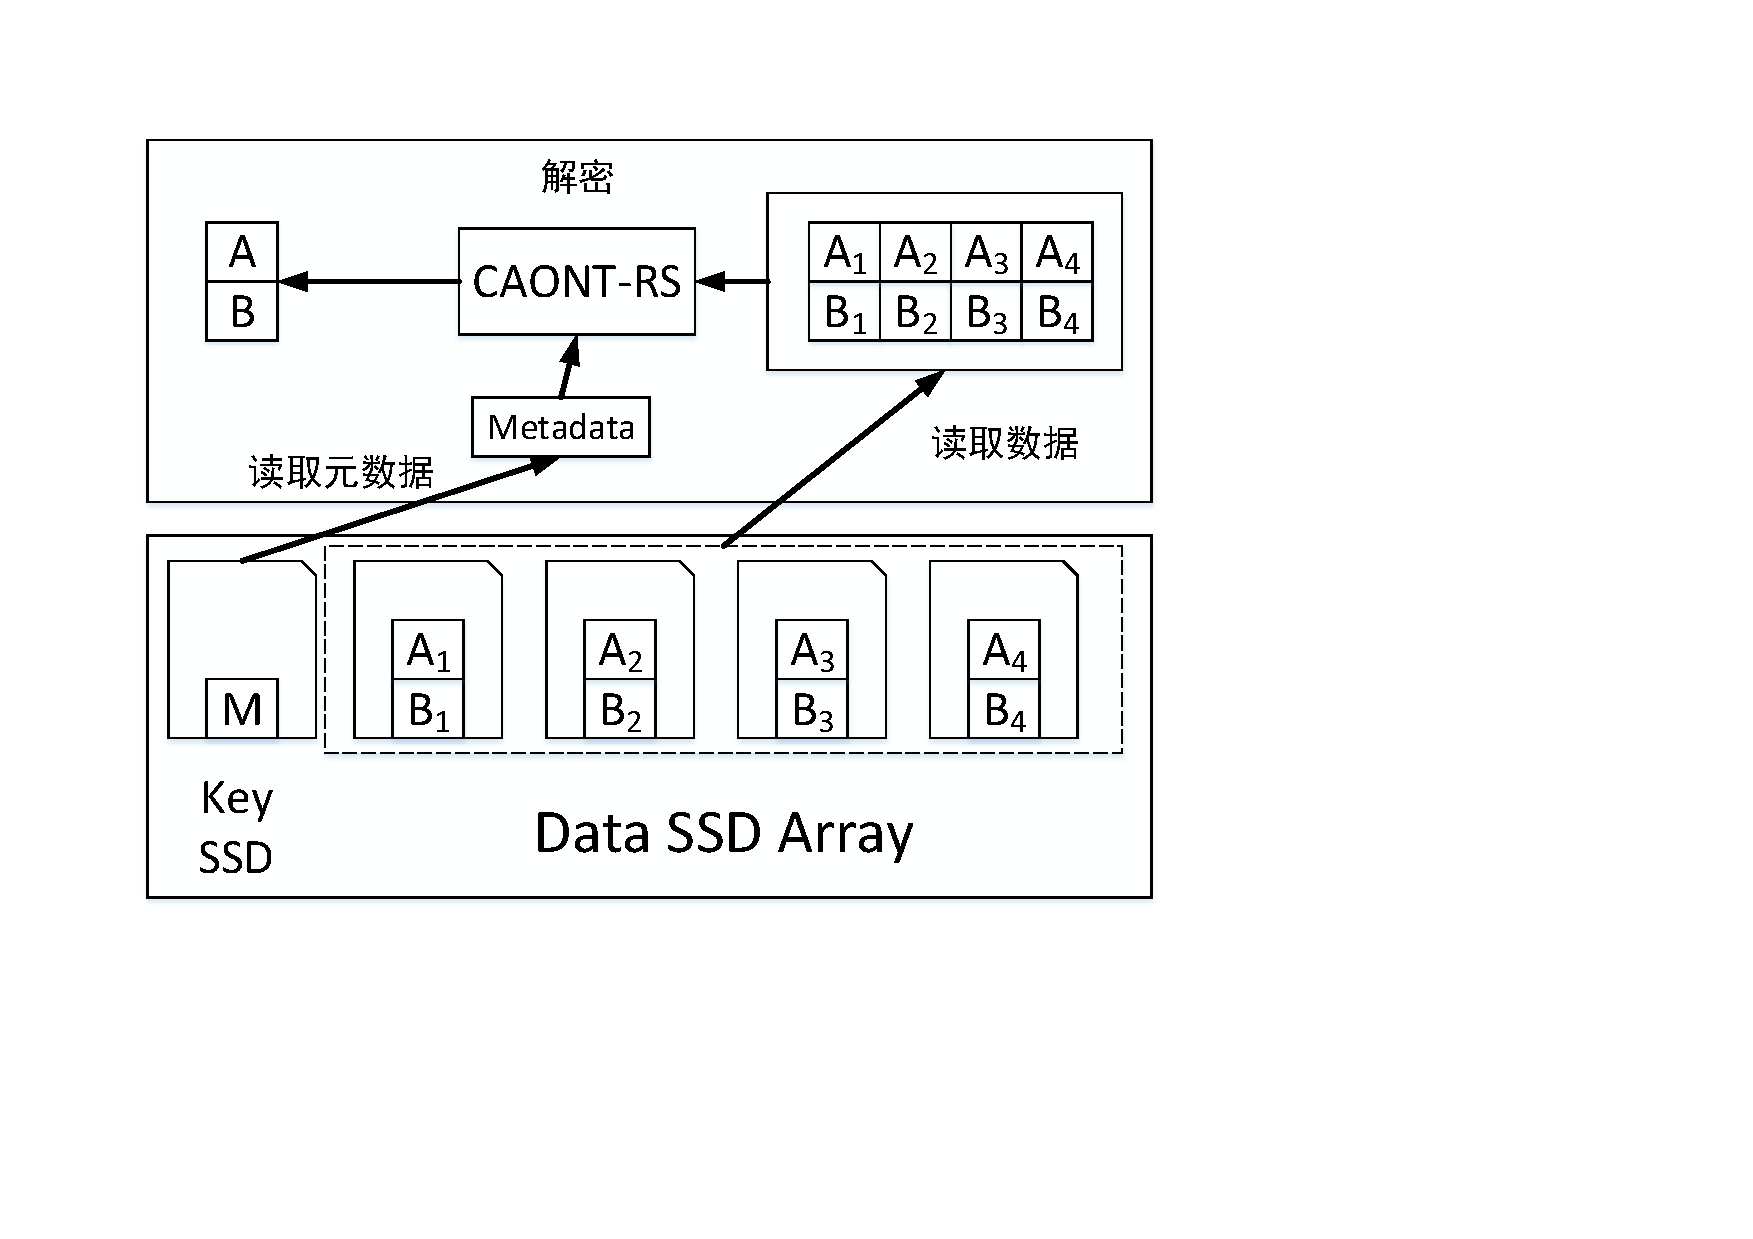
\includegraphics[width=4in]{Pics/data-read-st.pdf}
	\caption{数据读取架构}
    \label{fig:11}
\end{figure}
\begin{figure}[H]
	\centering
	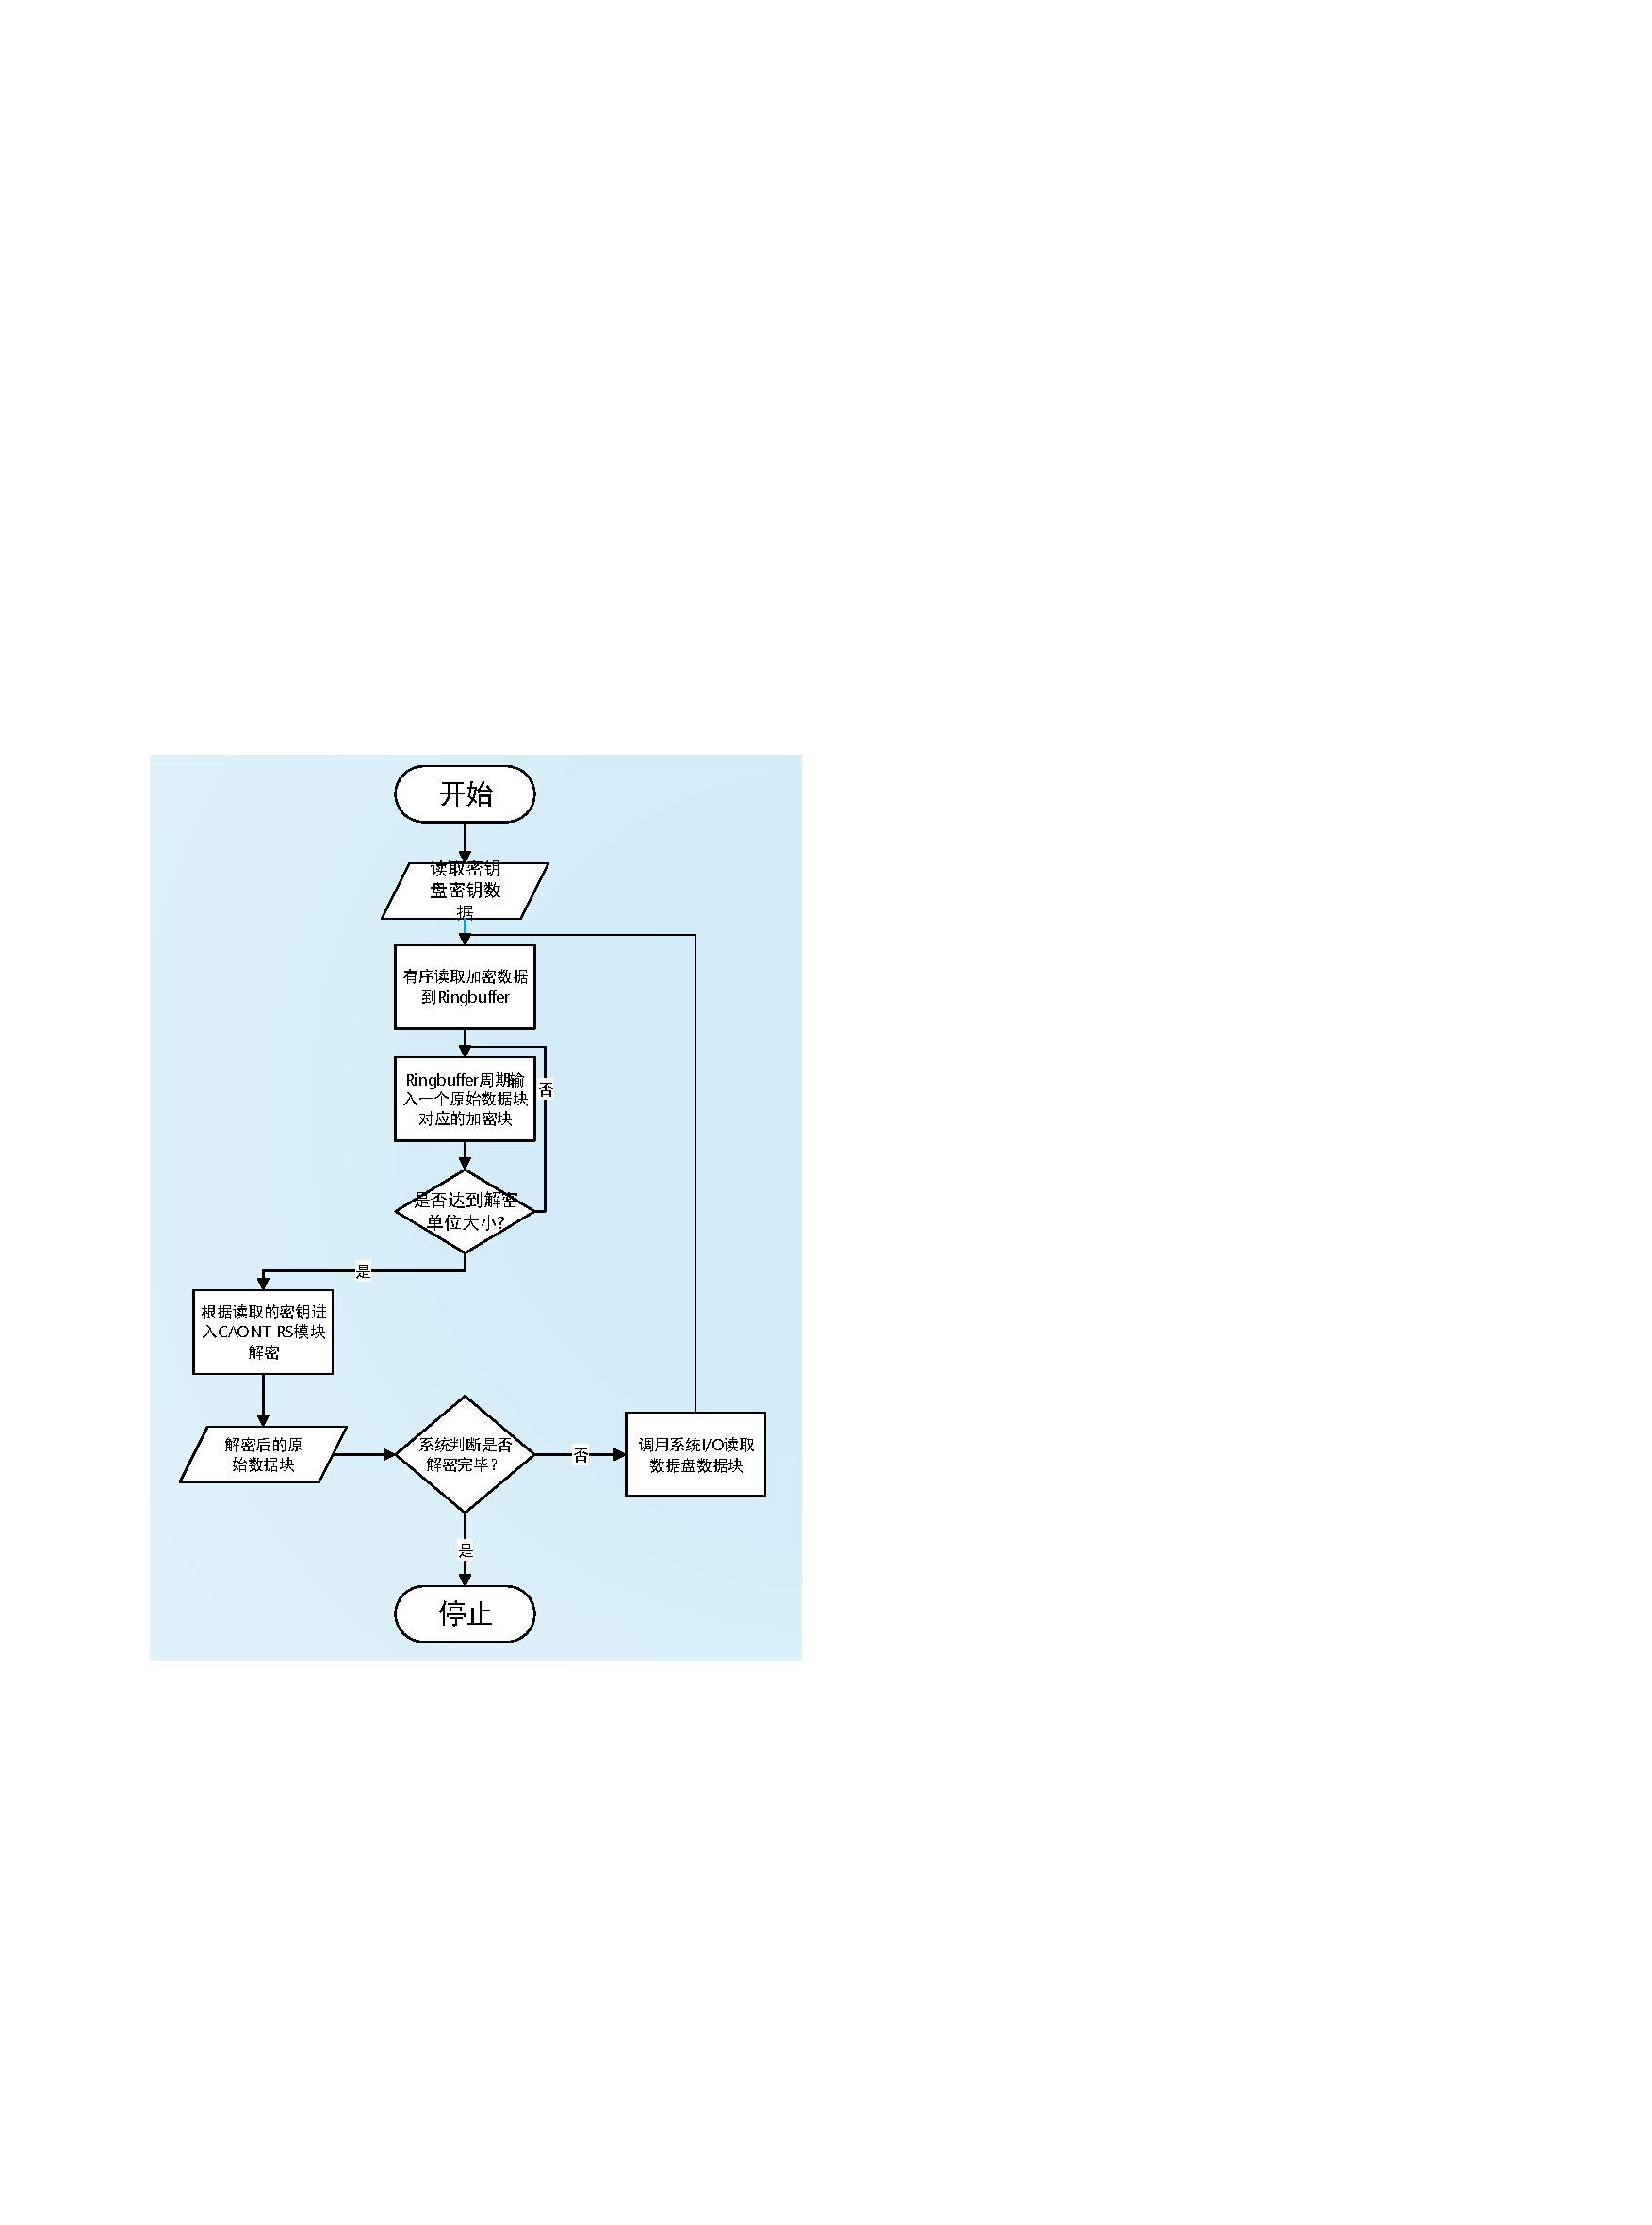
\includegraphics[width=4in]{Pics/data-read-pr.pdf}
	\caption{数据读取流程}
    \label{fig:12}
\end{figure}
在\autoref{fig:11}所示的数据读取结构和\autoref{fig:12}的数据读取流程中,当需要读取原始数据时,密钥模块首先读取密钥盘上的数据,初始化密钥。然后数据分发模块按照次序读取各个数据盘上的加密单元数据,并缓存在循环队列里。当数据符合解密单元大小时,加密模块利用数据和密钥解密出原始数据块。系统处理完加密数据后,原始数据已被全部解密还原,数据读取流程结束。
\subsection{安全删除密钥数据}
由于每个单位大小的原始数据块的哈希信息很小,因此相比加密后的数据块来说,原始数据块的哈希信息等这些密钥相关的数据量很小,在密钥盘上存储的区域范围也很小,针对密钥盘的全盘擦除所花费的时间很少,而且,擦除数据时,真正有用的部分也只是针对这一块区域的数据进行覆写,从密钥盘的闪存使用寿命角度来说,这部分的擦除数据对于整体的固态盘擦除寿命影响很小。
\begin{figure}[H]
	\centering
	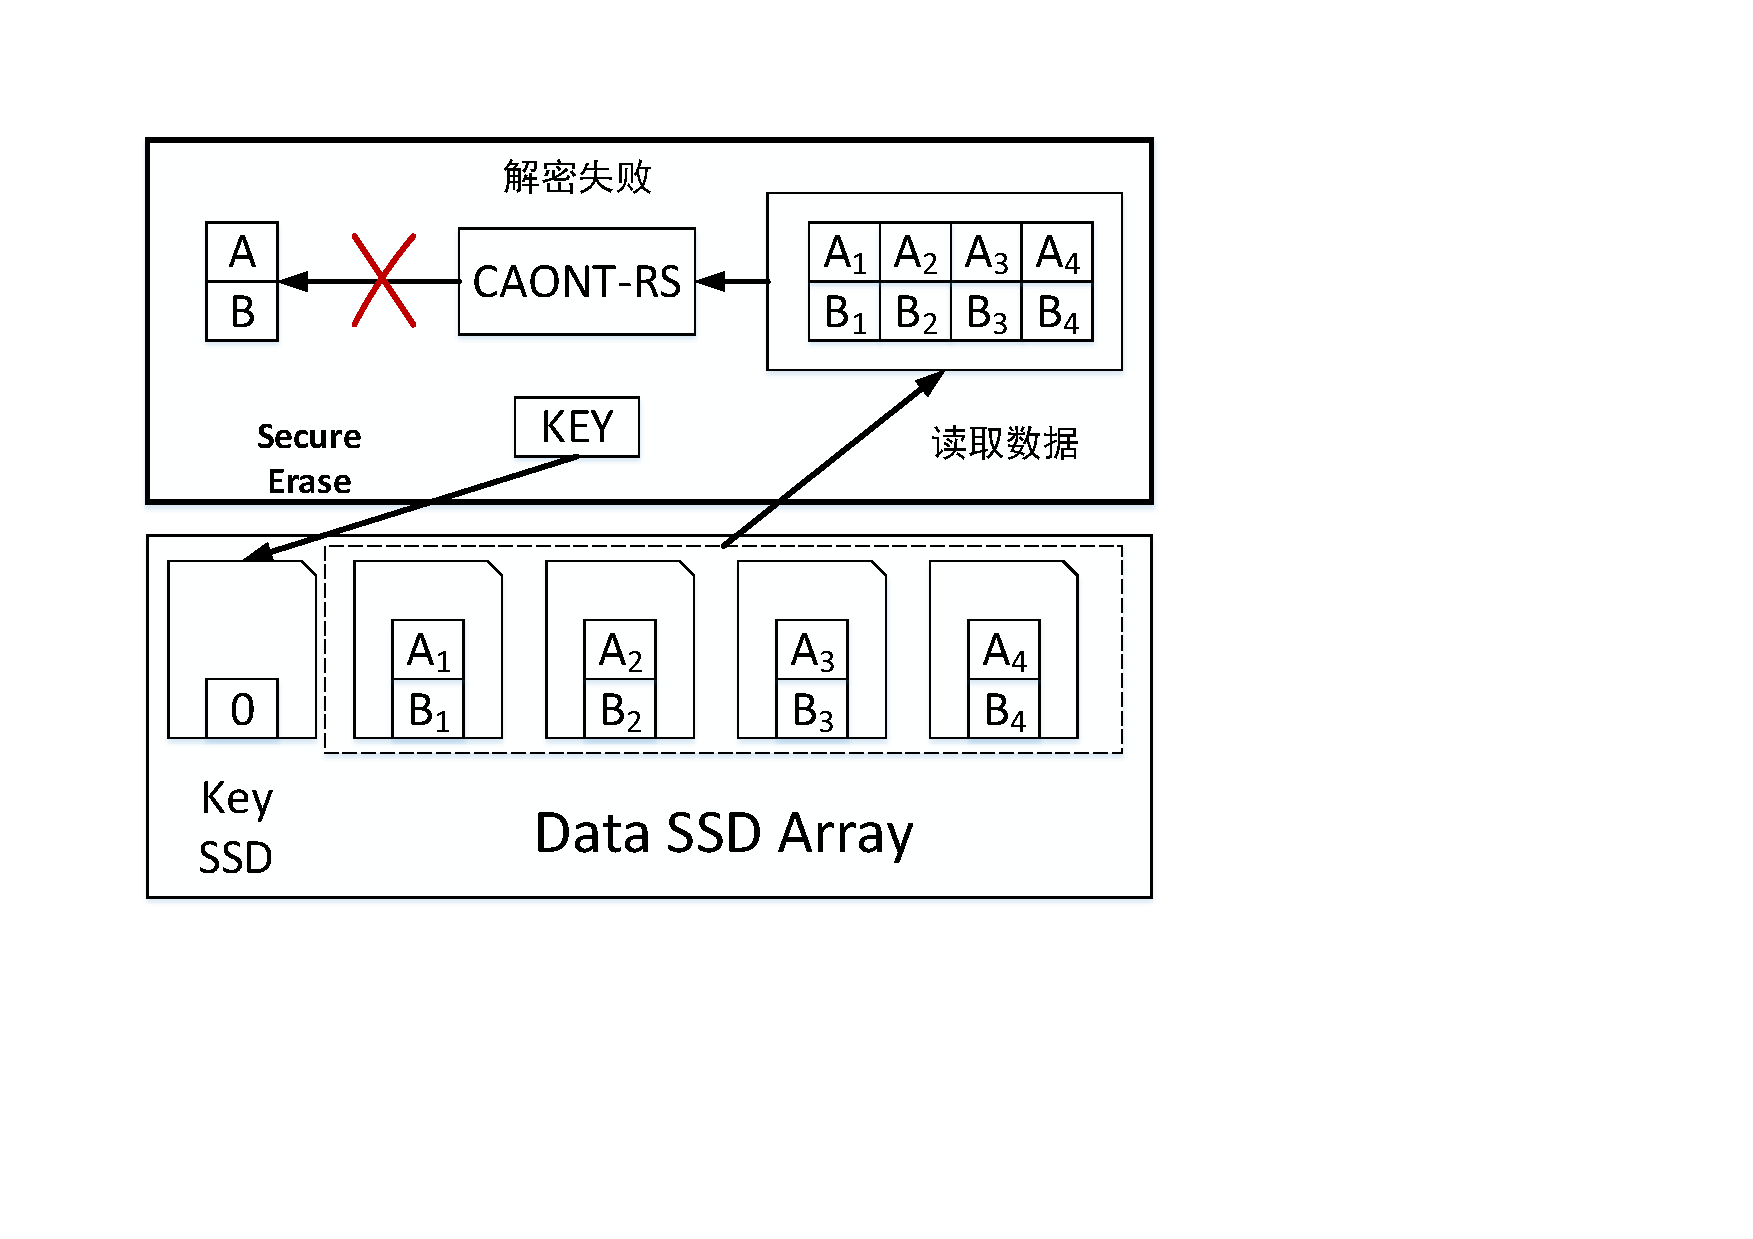
\includegraphics[width=4in]{Pics/del-key-st.pdf}
	\caption{擦除哈希信息验证读取架构}\label{fig:13}
\end{figure}
\begin{figure}[H]
	\centering
	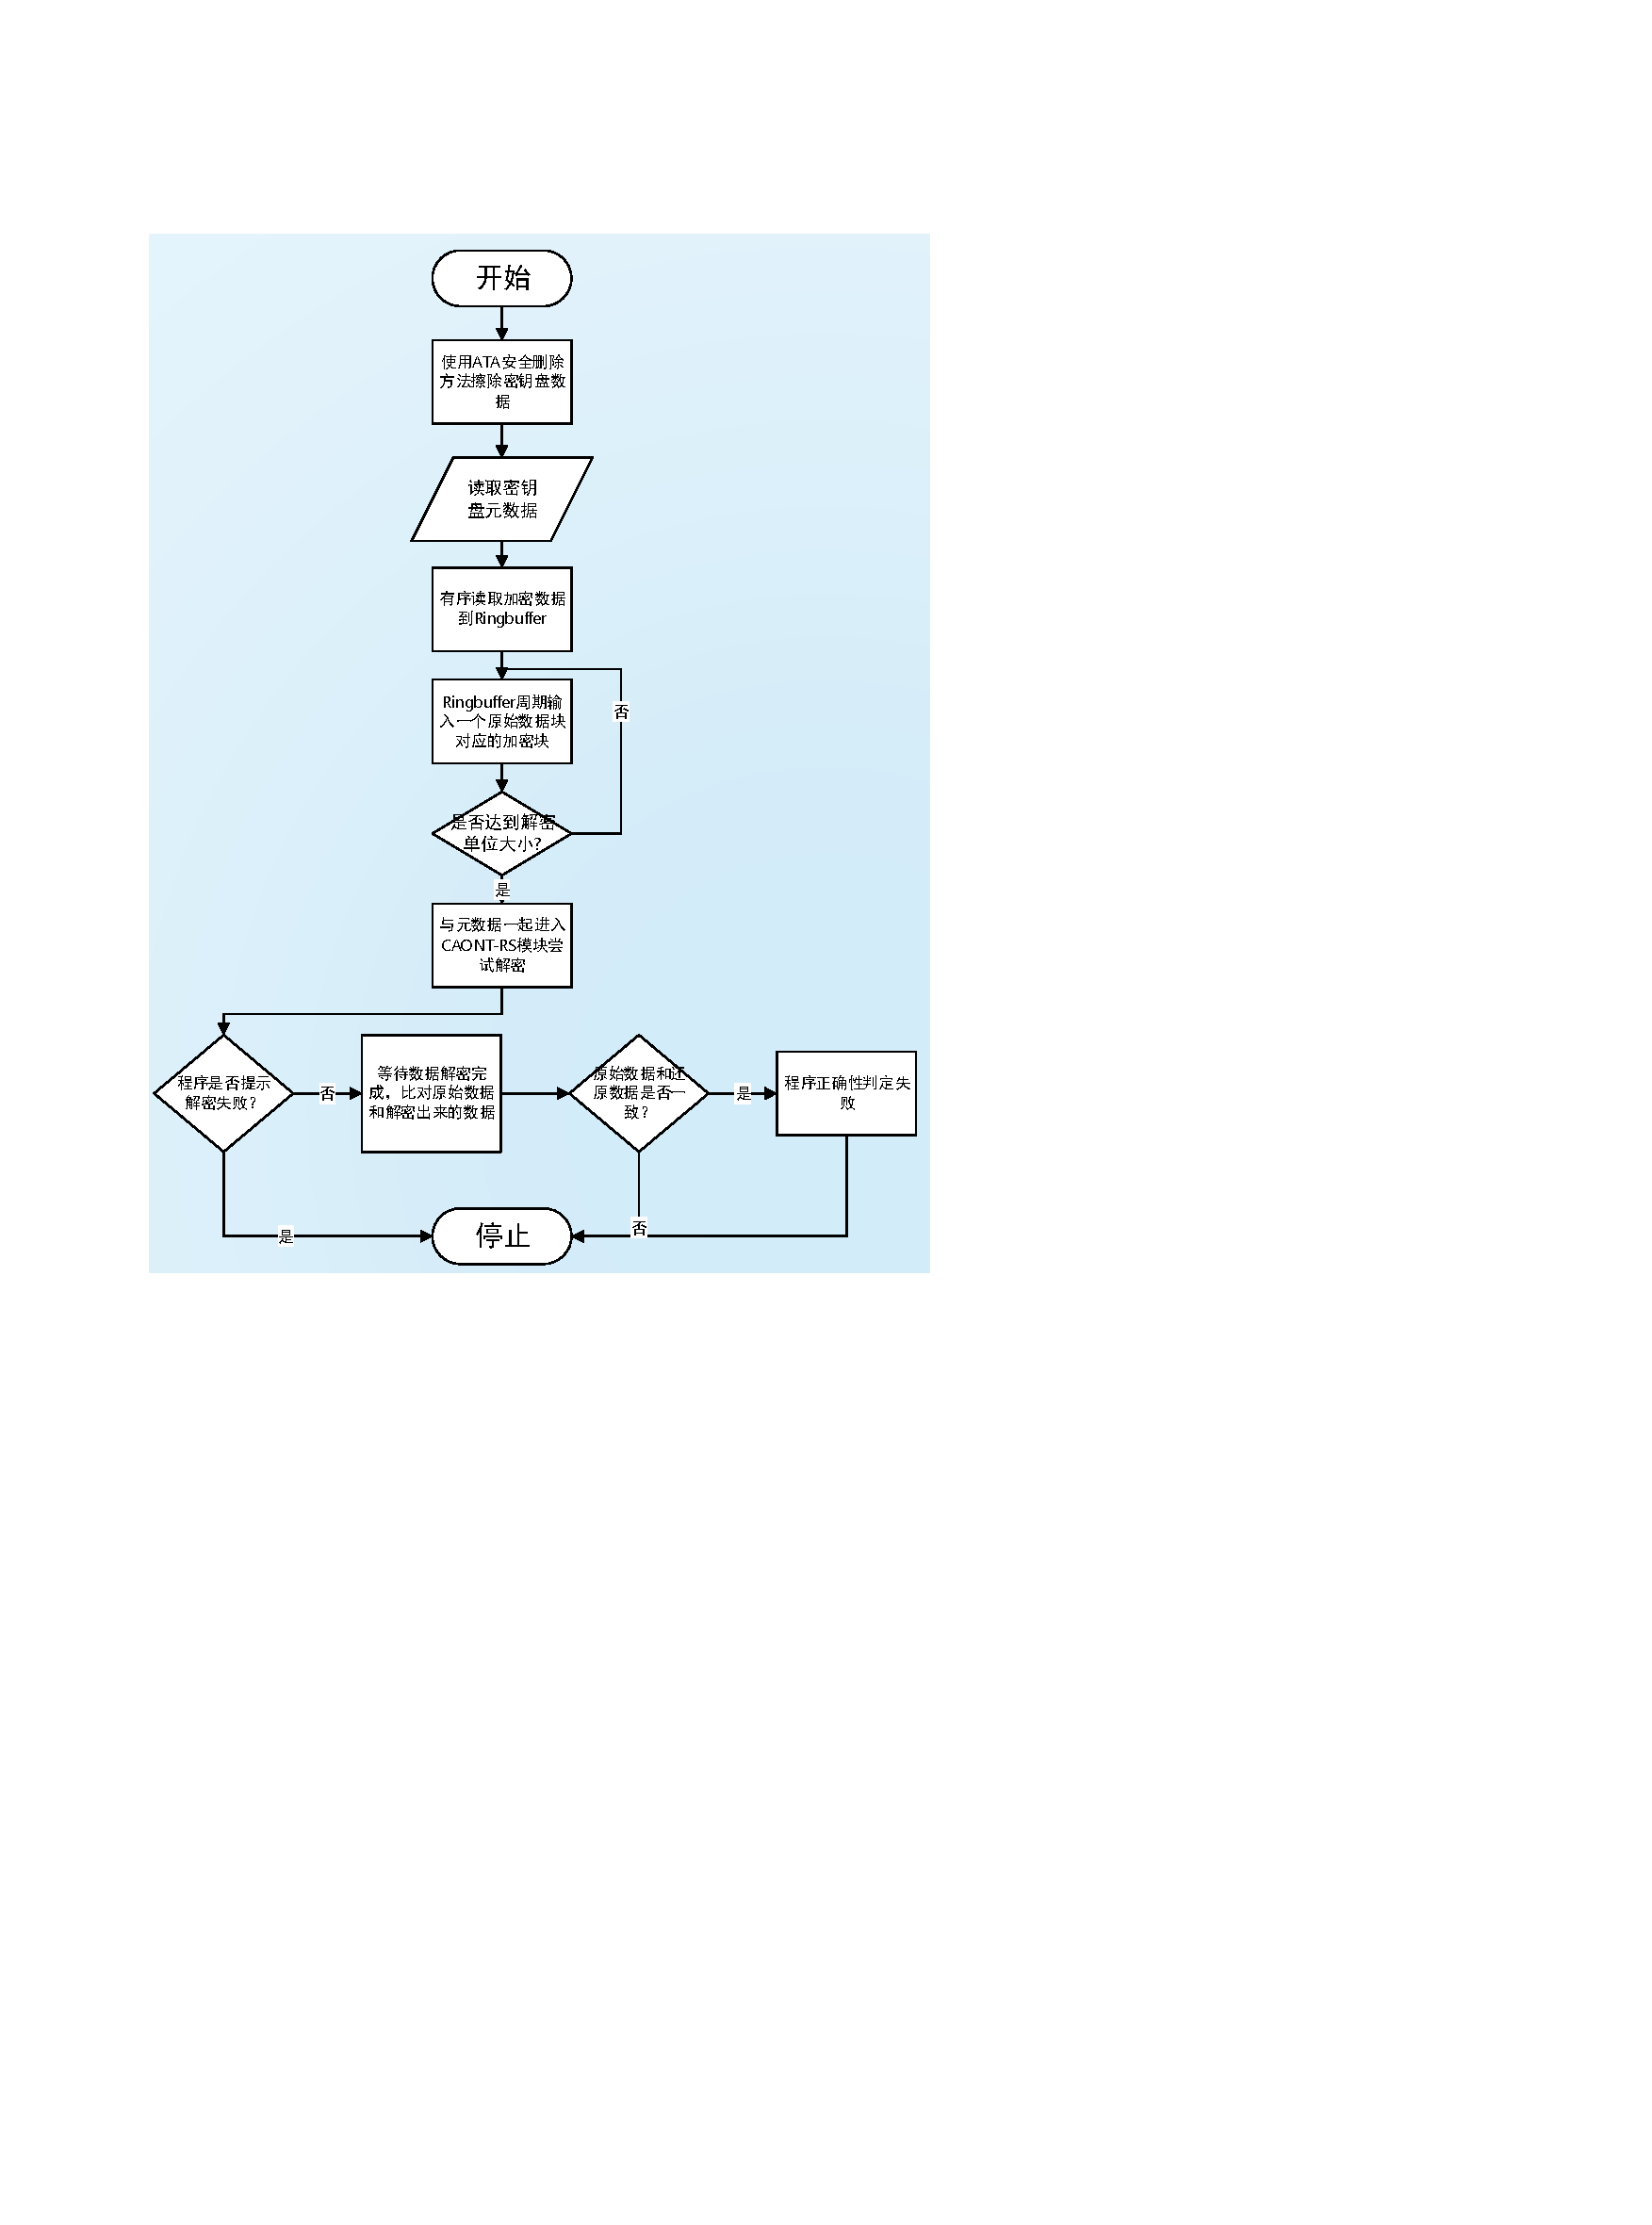
\includegraphics[width=4in]{Pics/del-key-pr.pdf}
	\caption{擦除哈希信息验证读取流程}\label{fig:14}
\end{figure}
在\autoref{fig:13}所示的删除密钥信息以及\autoref{fig:14}的删除后验证读取流程中,对密钥盘进行数据覆写时,使用了固态盘物理页复写的技术。即美国加利福尼亚大学的研究人员通过实验证实\cite{Wei2011Reliably},目前市面上的 SLC 闪存基本都支持覆盖写入(只能将 1 改成 0),即可以在擦除前对物理页进行复写(即第二次写操作),而对闪存的错误率并不产生明显的影响。
因此整个擦除手段如算法\autoref{alg:1}进行,在上层系统激活了删除功能时,系统立即调用密钥盘的TRIM命令标记密钥盘无效数据操作,然后针对密钥盘采取多次全盘覆写操作,具体操作如\autoref{fig:14}所示的擦除实现:首先使用安全擦除工具擦除密钥盘上的全部数据,这种擦除手段是先向每一个物理页覆写数据0,然后再次向物理页覆写随机数据,最后覆写一次数据0,达到安全删除的目的。
\begin{algorithm}[H]
\caption{Secure Erase data Hash informathons.(Key data)}
\label{alg:1}
\begin{algorithmic}
	\REQUIRE
	$addr$: address of the NAND flash page;
	$i$: position of page
	$data$: page content
	\STATE {// 1. write zero to each page}
	\STATE $data \gets 0$
	\FOR{$i=0$ to SSD page total size}
	\STATE write data to page $addr_i$
	\ENDFOR
	\STATE // 2. write random bit to each page
	\FOR{$i=0$ to SSD page total size}
	\STATE write random bit to page $addr_i$
	\ENDFOR
	\STATE // 3. write zero to each page again.
	\STATE $data \gets 0$
	\FOR{$i=0$ to SSD page total size}
	\STATE write data to page $addr_i$;
	\ENDFOR
\end{algorithmic}
\end{algorithm}


此时密钥盘上的数据位全部恢复了初始值,然后密钥模块读取密钥数据,同时数据分发模块获取每个数据盘上的加密数据,放入循环队列中缓存,加密模块尝试对数据进行解密操作,如果出错则说明密钥数据已经被更改,有效地阻止了数据被还原出来。如果解密流程正常进行,则比对最后被还原的数据和初始的数据内容,两者不一致则说明系统安全删除功能正常,否则判定失败。

\section{本章小结}
本文是全文的重点之一,旨在阐述全闪存盘阵的数据安全删除方案的设计,首先介绍了方案依赖的前提和安全删除的技术关键,
然后按照方案的各个模块定义介绍了数据加密方法,破坏数据恢复的条件以达到安全删除的目的,最后依次详细介绍了写入、读取、安全删除数据这些功能的架构和流程。

\chapter{仿真系统实验设计}
本方案是将原始数据块的哈希信息等密钥相关的数据存放在单独的固态盘上,要求这种固态盘內建的TRIM和安全删除命令已经被厂商正确地实现,而加密后的数据是存放在以固态盘组成的阵列上的,每个加密数据单元存储在阵列的一个条带上,写入数据的时候按照方案设计的缓存模块,依次顺序写到每个条带上,读取的时候,由于输入缓存支持并行传输,利用了阵列并发IO的特点,快速读取到缓存中并且按序存放。要使得原始数据无法再被恢复,擦除掉密钥盘上的哈希信息,或者破坏方法预设的条带数量临界值的数据,就可以达到数据安全的结果。


采用本方案可以实现多种原型系统,例如,基于iSCSI平台,原始数据经过方案实现的系统加密,产生的加密数据分发到以TCP/IP相互连通组成的阵列上,解密数据时只要通过网络读取到各个存储点上的加密数据以及存储在单个盘上的哈希信息,完成解密操作即可。


为了方便验证方案,实验选择了环境相近的仿真实现。仿真实验环境也要求有一个单独的闪存盘用以存储加密的哈希信息参数数据,并且这个固态盘能够做到数据的安全删除,以及TRIM命令的內建实现,为了容易实现,是在以固态盘组成的阵列上划分分区,成为一个个独立的存储单元来存放加密之后的数据单元这种设计,来完成仿真实验。
\section{实验目的}
采用仿真实验主要有以下三个方面的目的:
\begin{itemize}
	\item 确认方案能够达到盘阵数据安全删除的要求。具有可行性。
	\item 仿真测试不同安全级别下,方案在带宽、I/O时延、系统负载、数据冗余率等维度的性能表现,验证方案是否可靠。
	\item 通过较容易实现的仿真环境来进行测试,确保方案针对所有固态盘阵都具有可用性。
\end{itemize}
\section{实验环境}
仿真实验环境硬件配置如\autoref{tab:2}所示。
\begin{table}[H]
    \centering
    \caption{实验环境硬件配置}
    \label{tab:2}
    \begin{tabular}{|c|c|c|}
        \hline
        类别 & 型号 & 数量 \\ \hline
        CPU & Intel(R) Xeon(R) L5520  @ 2.27GHz & 16 \\ \hline
        内存 & 16GB & 1 \\ \hline
        密钥盘 & SV300S37A 120G & 1 \\ \hline
        数据盘 & SV300S37A 120G & 4 \\ \hline
    \end{tabular}
\end{table}
\section{实验方案}
本次仿真实验使用了4块SSD组成的阵列,然后分为4个独立存储区域作为冗余加密数据的存放点。一块单SSD盘作为密钥存储盘。数据块信息虽加密块信息分散存储在数据盘阵上。整体测试流程如\autoref{fig:15}所示。
\begin{figure}[H]
	\centering
	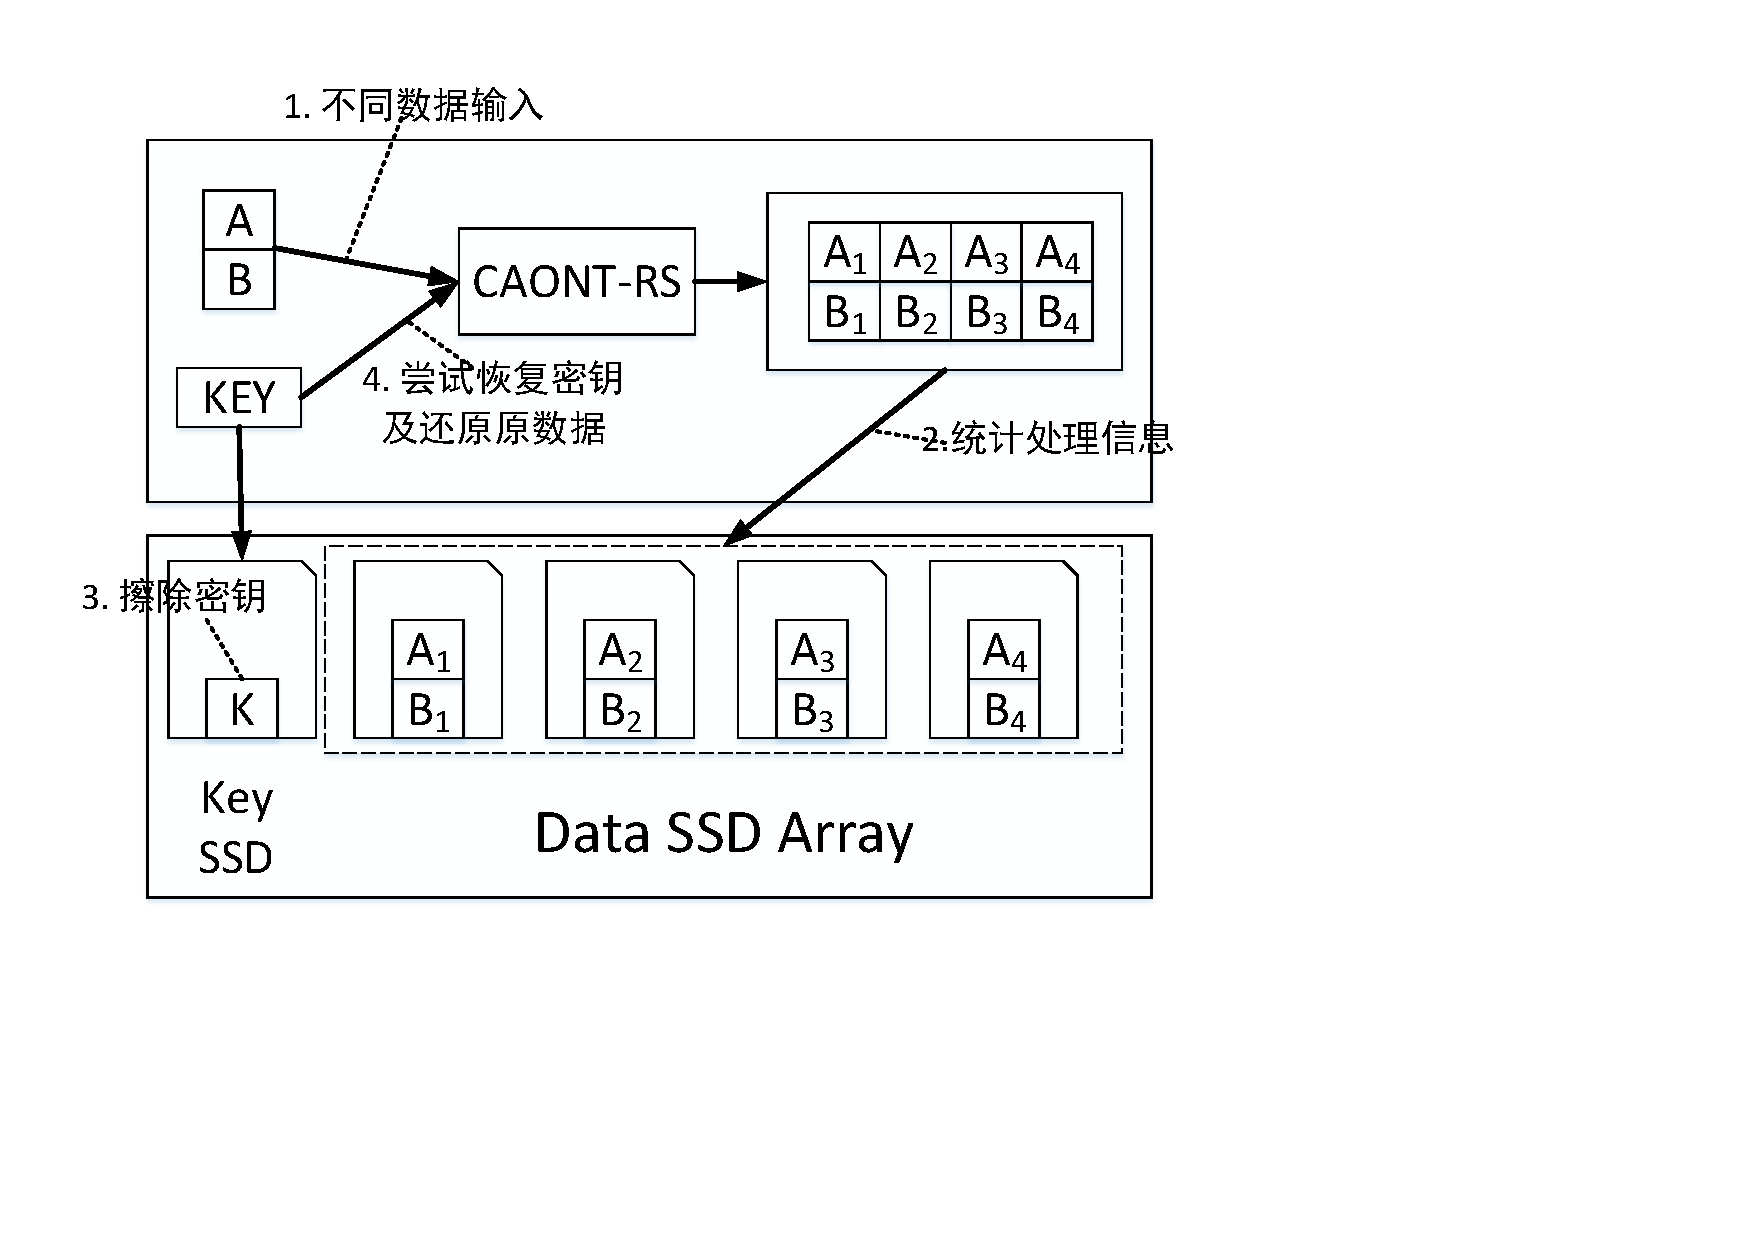
\includegraphics[width=4in]{Pics/test-pr.pdf}
	\caption{测试流程}
	\label{fig:15}
\end{figure}
\begin{enumerate}
	\item 从1MB到1024MB大小的原始数据依次输入仿真系统中
	\item 记录数据从读取到第一块数据被冗余加密,分发到阵列的过程中每个环节所消耗的时间,生成数据的大小以及系统运行状态等相关数据
	\item 记录加密数据读取到被加密模块解密,最终还原为原始数据的各个环节的时间、状态等数据
	\item 使用经过验证的安全删除软件将存储的密钥盘的哈希信息等数据擦除,尝试还原数据,验证安全删除功能
	\item 统计仿真系统测试数据,得到功能测试和性能测试等结果
\end{enumerate}
仿真环境结构如\autoref{fig:16}所示。
\begin{figure}[htb]
	\centering
	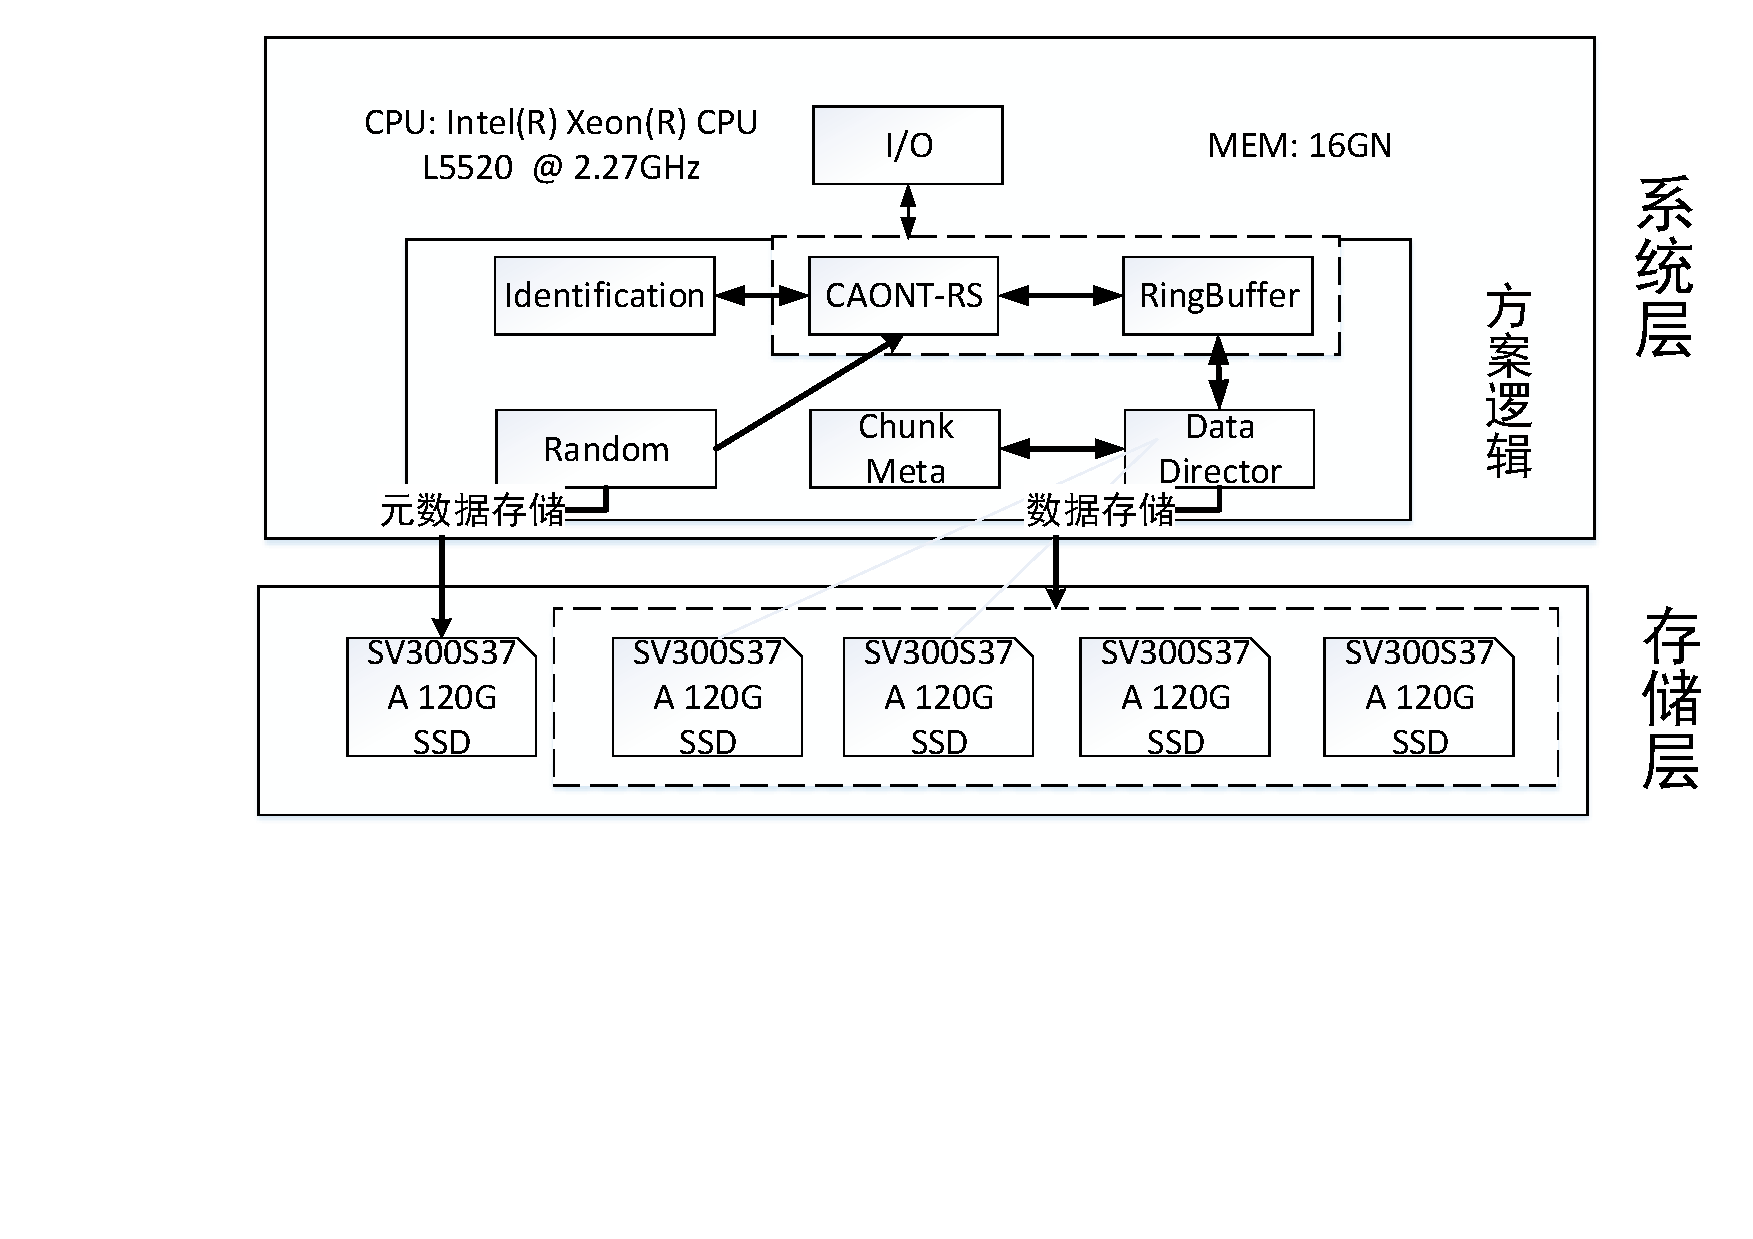
\includegraphics[width=1\textwidth]{Pics/test-env.pdf}
	\caption{仿真环境系统图}
	\label{fig:16}
\end{figure}
\section{仿真系统实现}
\subsection{数据结构设计}
数据结果部分,编码和解码的逻辑处理单元都有两个分别处理输入和输出的数据缓存中心,而这两个缓存中心得数据结构都是以线程安全的循环队列为中心,因此,设计一个多线程高效的循环队列成为了提高数据缓存效率的关键。\autoref{fig:17}和\autoref{fig:18}分别代表了编码输入缓存和输出缓存。
\begin{figure}[H]
	\centering
	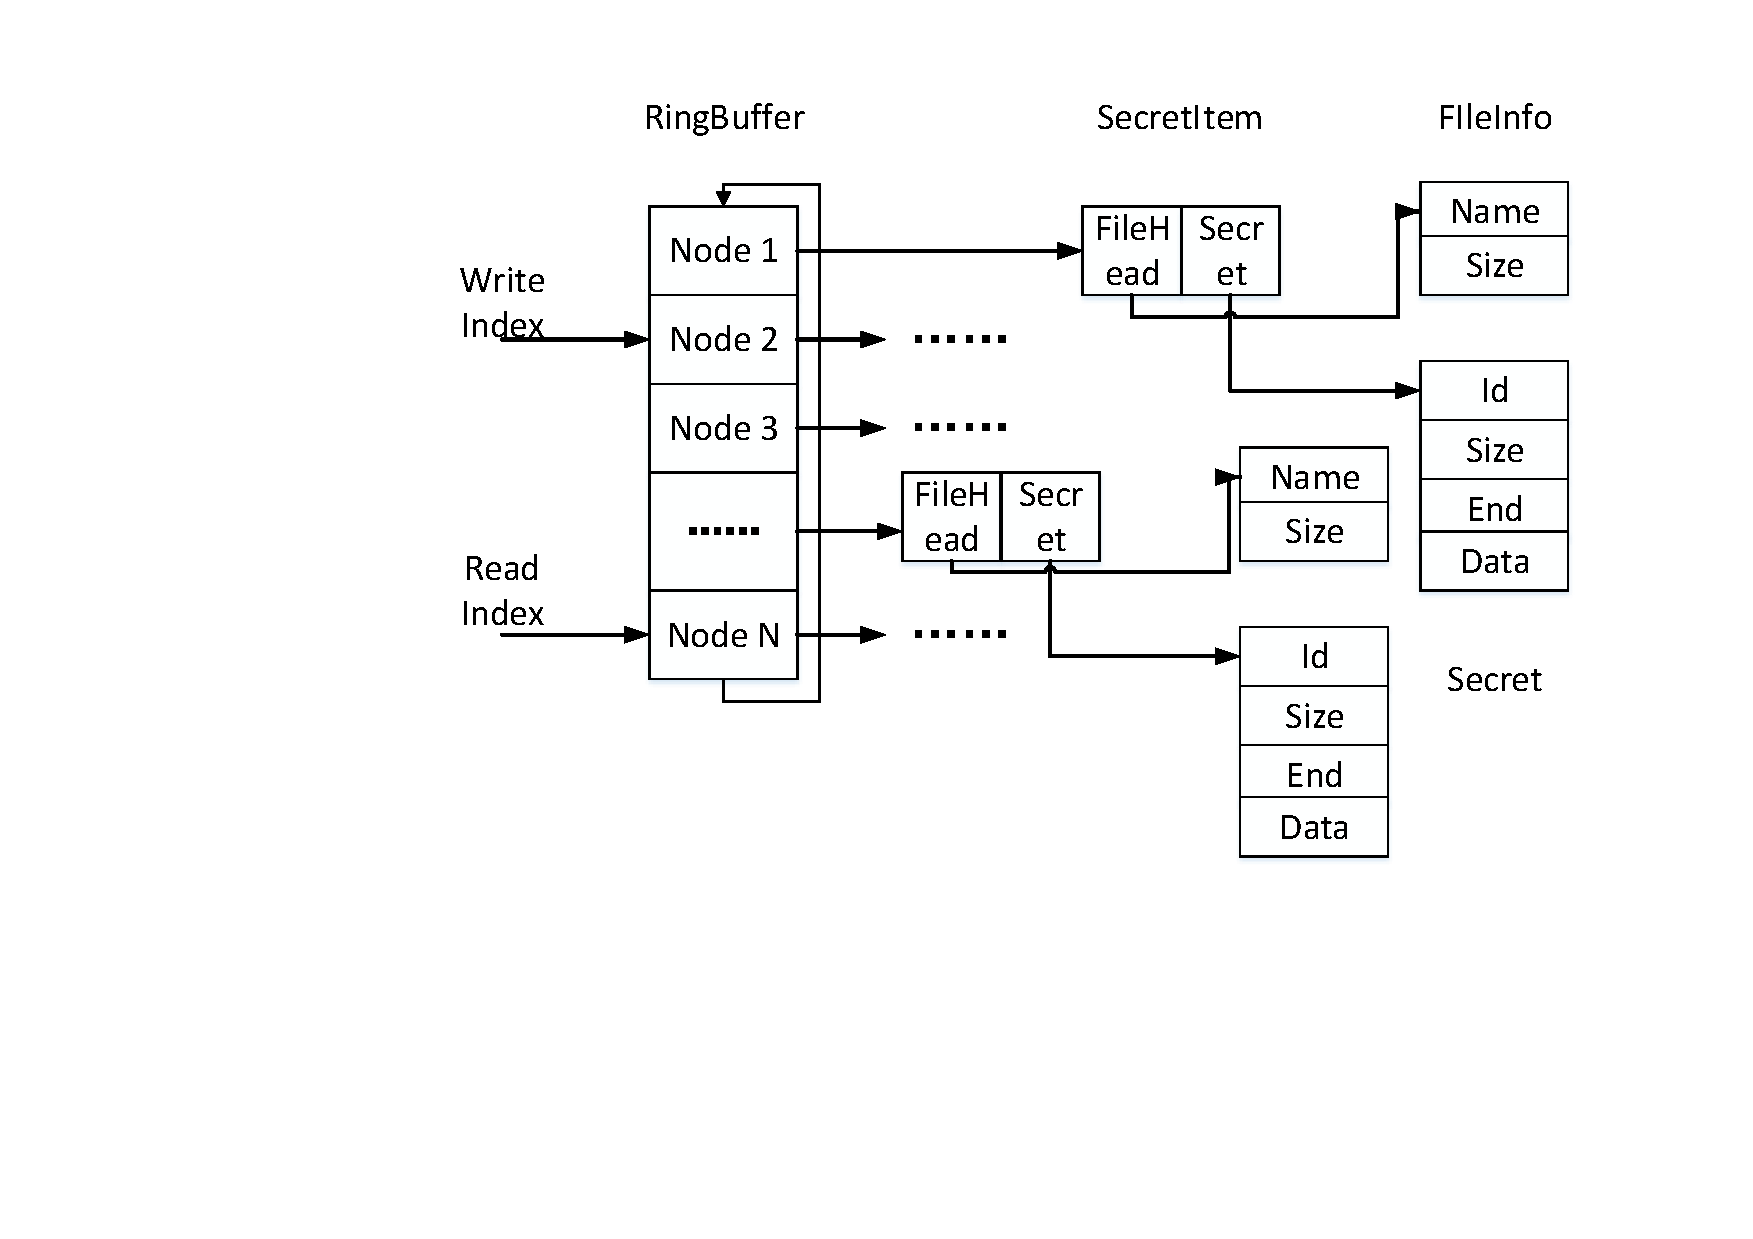
\includegraphics[width=1\textwidth]{Pics/input-buf.pdf}
	\caption{输入缓存数据结构设计}
	\label{fig:17}
\end{figure}
\begin{figure}[H]
	\centering
	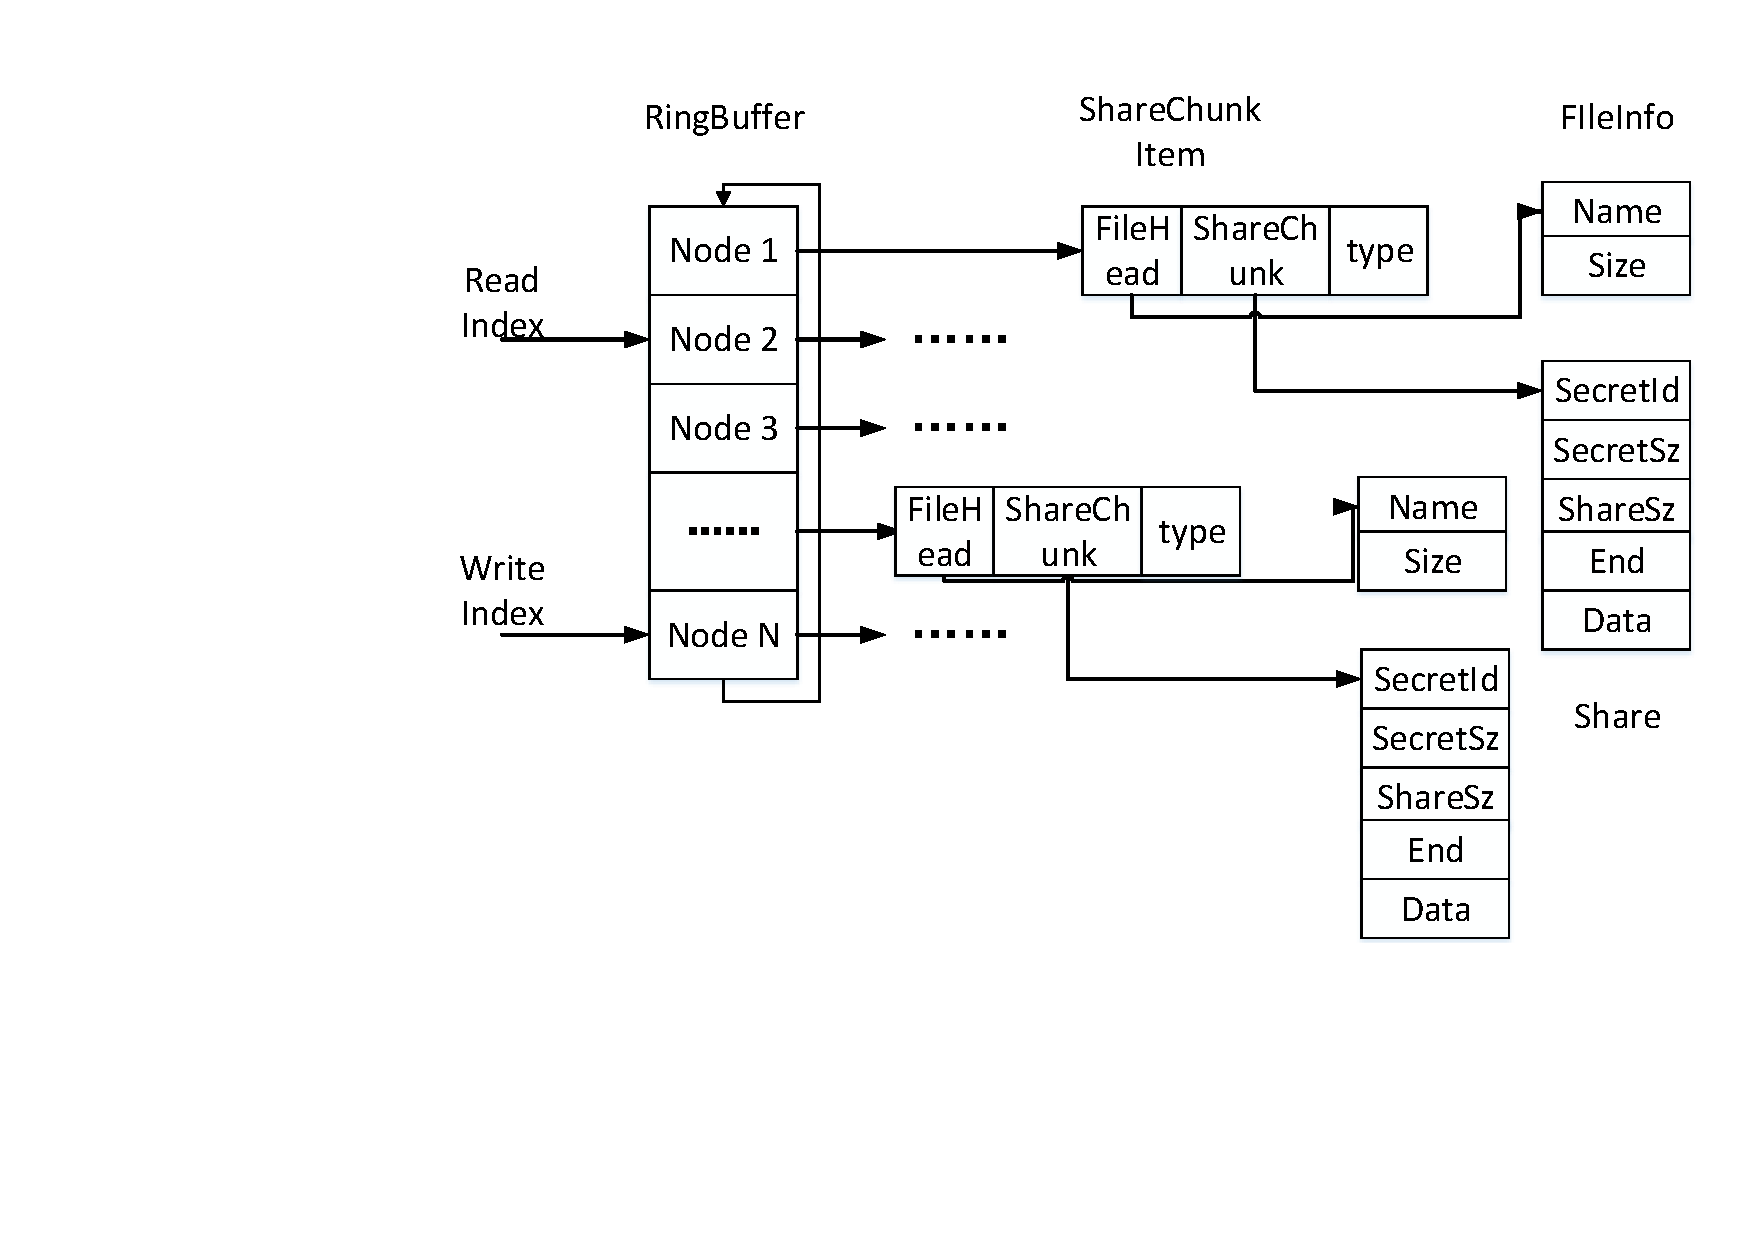
\includegraphics[width=1\textwidth]{Pics/output-buf.pdf}
	\caption{输出缓存数据结构设计}
	\label{fig:18}
\end{figure}
在数据进行编码时,使用如\autoref{fig:17}所示的缓存数据结构,当一个数据块被加密处理完,生成加密数据块后,循环队列在当前写结点开辟一个新的内存,存放原始数据块的文件名、文件大小信息,加密子结点指向一个加密块的序号Id,大小Size,是否是最后一个加密块的标志End,以及最终的加密数据块Data,同时,写索引向后移动一个结点位置,这样一个加密块的缓存过程就结束了。如果写索引后面是读结点,说明队列的缓存已满,队列将在接下来的一段时间拒绝数据缓存请求。


当缓存需要写入到数据盘时,循环队列的读索引获取加密数据块的Id,按照数据盘的个数取模,决定存储在哪个数据盘,队列将当前的读结点的数据传递给数据存储线程,读索引向后移动一个结点位置,缓存读取过程结束,如果读索引后面位置是写结点,则表明当前循环队列已空,接下来的一段时间内数据存储请求将被队列忽略,相关线程也会陷入休眠,知道有数据到达。


加密数据解码时,使用的是如\autoref{fig:18}所示的缓存结构,相关的读写操作刚好和编码相反,只是输出缓存的相关结点内容发生了变化,首先是队列的结点指向的是一个原始文件信息和加密数据块联合的结构体,由类型标明这是一个数据块还是信息块,其中数据块部分相比编码前是多了一个表示最终的冗余加密数据块的大小。数据块依然是由标记End标明是否是最后一个数据块,在数据解密流程起到通知模块解密结束的作用。
\subsection{关键流程实现}
%在方案设计的数据处理流程中,主要做了以下几个比较具体的实现和改进。
\subsubsection{将数据读写模式进行了改进优化}
为了提高系统处理数据的整体性能,除了设计一种比较高效的循环队列以外,方案还对数据存取的具体环节进行了优化设计。以实验系统中的四个数据盘来说,在编码过程中,编码器会将编码完成的数据按照其编号顺序依次存入各个盘对应的循环队列中,各个队列之间的数据缓存以及写入是相互独立的,这样带来的好处就是,相比一个循环队列,数据缓存和存储的数据同步冲突更小,线程切换的次数减少,从而可以并行地存储数据到各个数据盘。


同时在解码时,由于编码算法的特性,只需要读取k份数据即可将原始数据还原出来,具体到本方案中,相比编码需要传输四份数据单元,解码的时候只要读取其中任意三份数据,有效的节省了数据传输的带宽,也减少了等待数据缓存的时间,系统处理性能自然就提升上去了。整体流程架构如\autoref{fig:19}所示。
\begin{figure}
	\centering
	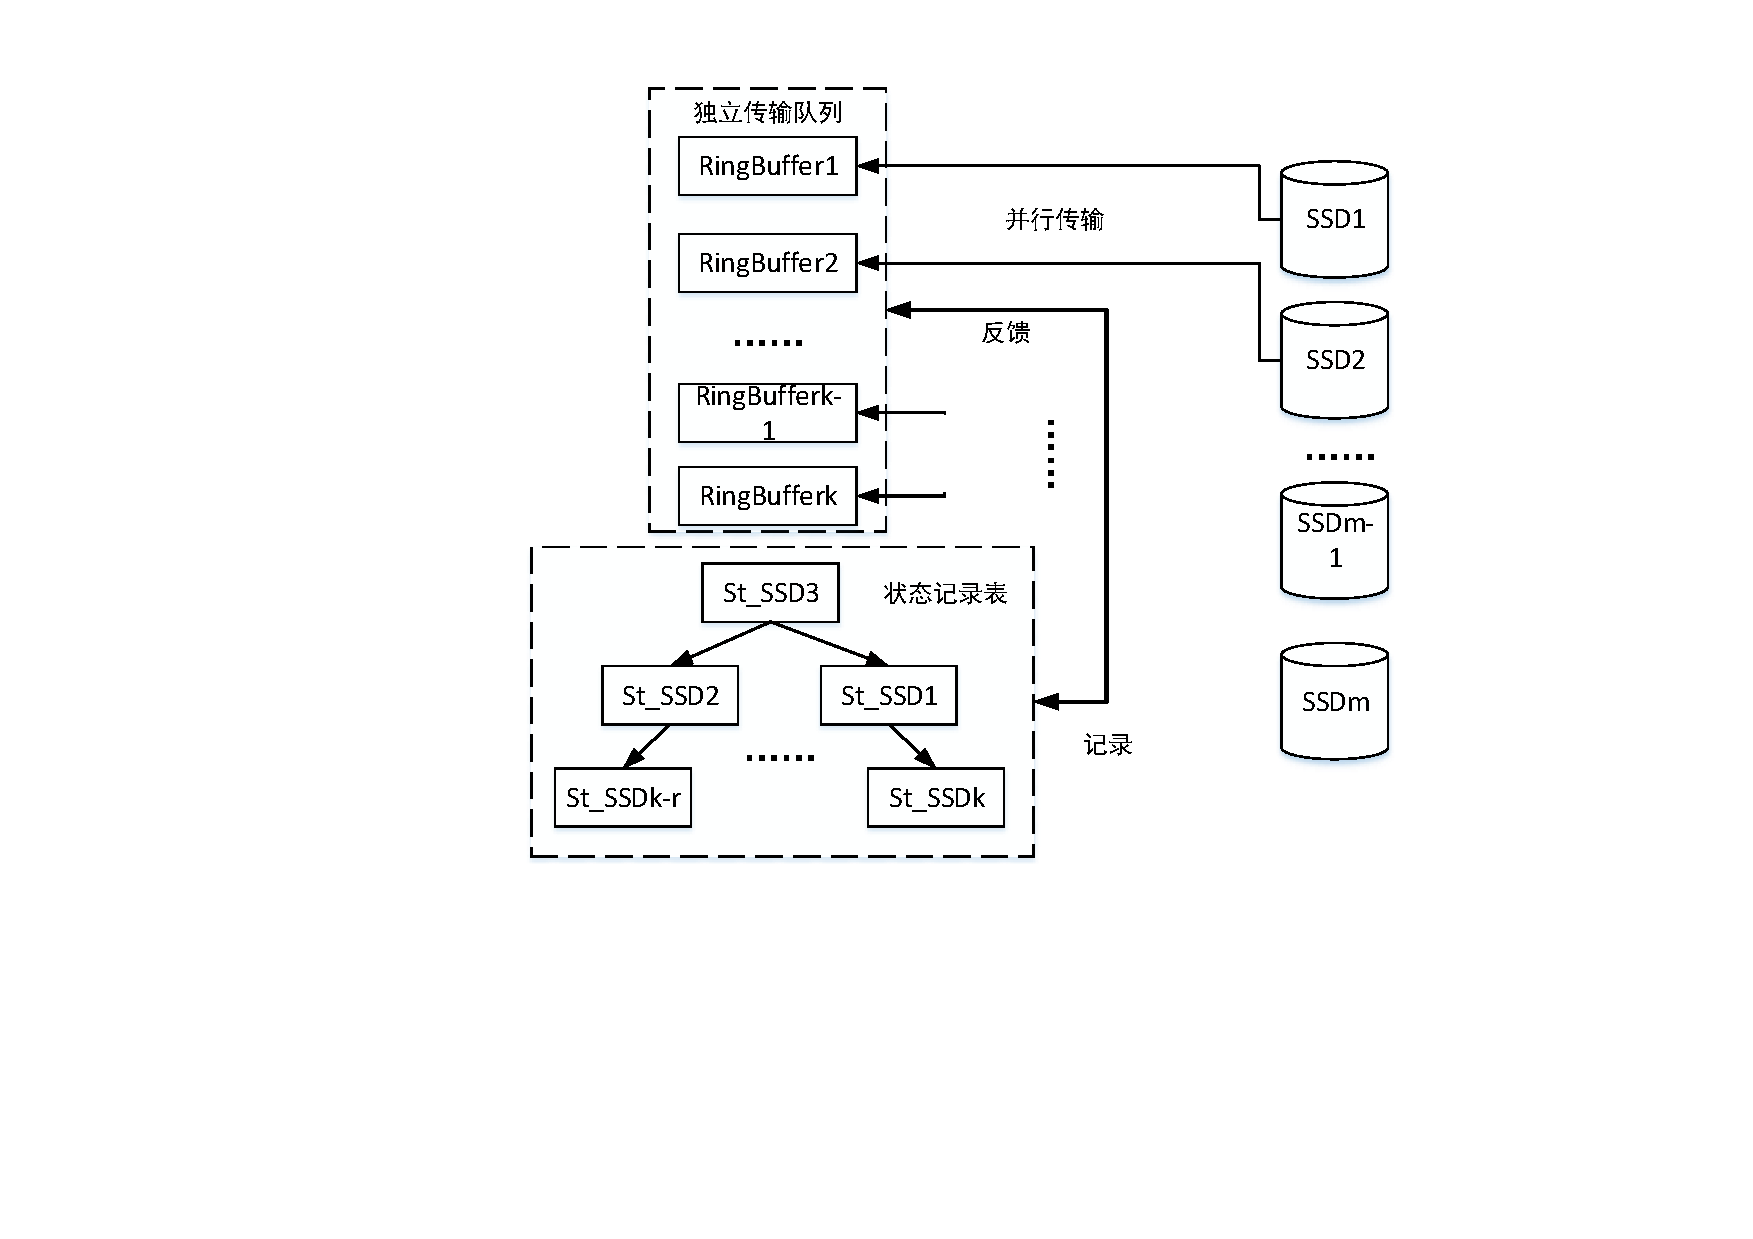
\includegraphics[width=1\textwidth]{Pics/parallel-read.pdf}
	\caption{输出缓存架构设计}
	\label{fig:19}
\end{figure}
另外一个改进是,每次传输数据时,系统都会记录下当前各个数据盘的状态,依据这个状态在那些综合性能比较好的数据盘上优先读取数据,这样带来的一个好处是,系统的容错性大大提升。以测试的4个盘为例,假使有1个盘损坏,也不影响数据读取还原,在比测试规模大很多的环境下,因为数据盘的损坏可能性比较明显,这种容错性带来的优势更加明显,数据的完整性也得到了保证。同时,系统选择那些性能较好的数据盘读取数据,也有效地避免了因为单盘影响其他所有数据盘读取性能的问题。
\subsubsection{实现了密钥数据存储到密钥盘的策略}
由于环境、操作系统等问题造成的不可抗力,都可能使得这套系统崩溃,由于初始密钥向量是随机化生成的,此时仍在内存中,就会因为系统崩溃而丢失,原始的数据无法再通过系统解密再恢复出来,造成了数据丢失。现有的设计对这一问题的解决方法是,在每次处理完数据加密后,密钥模块负责将本次生成的密钥数据存储到单独的密钥盘,设计的密钥存储结构如\autoref{fig:20}所示。
\begin{figure}[H]
	\centering
	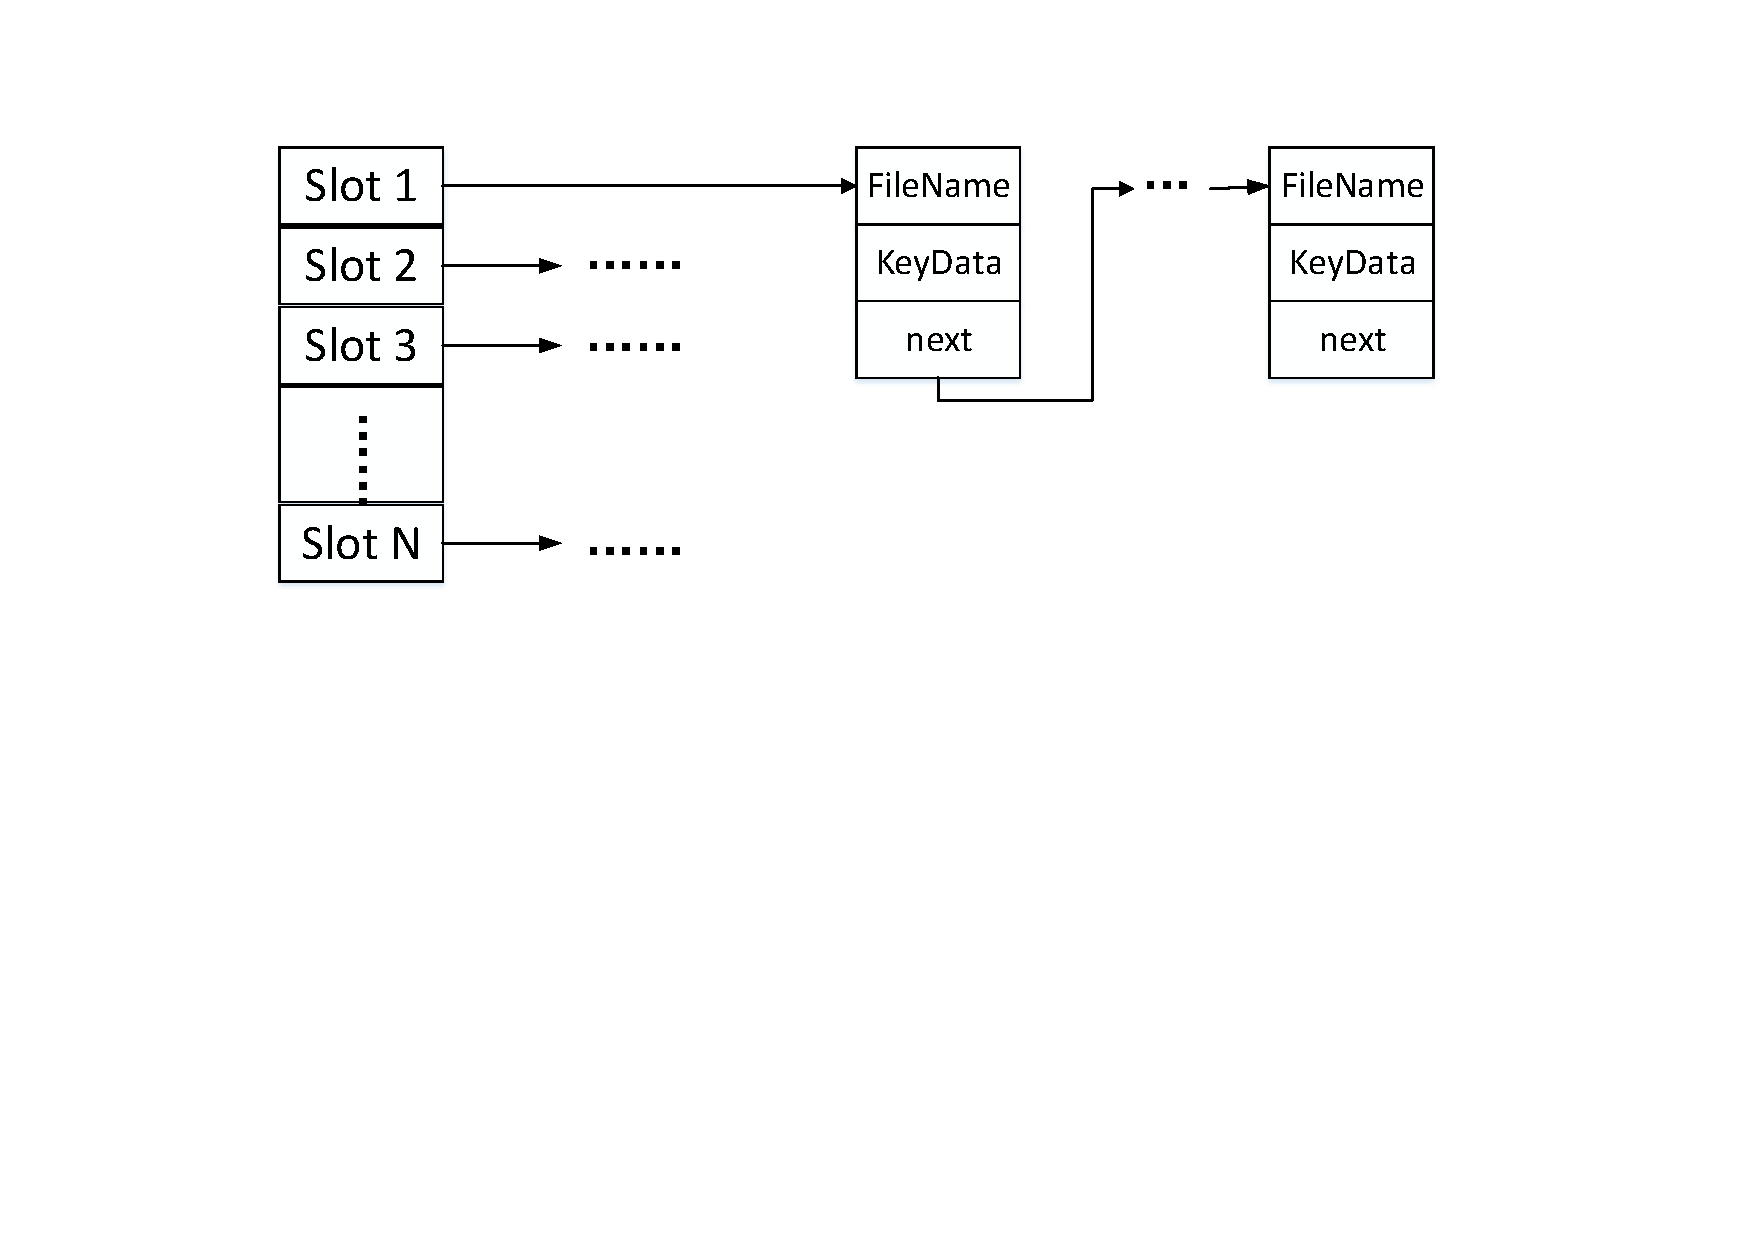
\includegraphics[width=1\textwidth]{Pics/keystore.pdf}
	\caption{密钥存储结构}
	\label{fig:20}
\end{figure}
这样,在系统重启后,对于存储过的文件信息,系统会优先在密钥盘中查找密钥信息,如果是读取还原数据,直接使用密钥信息即可,对于重新存储请求,只需要覆盖掉原来得记录即可。
\subsubsection{加密算法实现}
 \begin{algorithm}[H]
 	\caption{Encode origin data with hash info.}
 	\label{alg:2}
 	\begin{algorithmic}
 		\REQUIRE $secret buffer,m \ge k$
 		\STATE $B \gets bytesof per secret word$
 		\STATE $S \gets secret buffer size$
 		\STATE $A \gets aligned secret buffer size$
 		\ENSURE $A \le min\{(S+B) \% (B+K), B*(k-1) / (B*k+1)\}$ 
 		\STATE $shareSize \gets (A / B + 1) / k * B$
 		\STATE $aligned buffer \gets secret buffer$
 		\STATE $Key \gets Generate Hash with aligned buffer$.
 		\FOR{i = 0 to A}
 		\STATE $aligned size constant Array_i \gets i\&0xff$;
 		\ENDFOR
 		\STATE erasure coding data $\gets$ Encrypt with aligned size constant Array and hash info.
 		\STATE erasure coding data $\gets$ Galois Group multiply region hash info with value 1 and,step by B,adding by 1.
 		\STATE share buffer $\gets$ erasure coding data
 		\FOR{i=0 to m}
 		\FOR{j=0 to k}
 		\STATE $value \gets distribution_{k^2+k*i+j}$;
 		\STATE
 		share buffer $chunk_{k+i} \gets$ Galois Group multiply region,
 		share buffer $chunk_j$ with value ,
 		step by shareSize,adding by 1 $if j \neq 0 else 0$
 		\ENDFOR
 		\ENDFOR
 		\RETURN share buffer
 	\end{algorithmic}
 \end{algorithm}
加密算法\autoref{alg:2}中,关键的操作主要有,首先根据对齐的原始数据块生成它的哈希值,作为该数据块加密的密钥,使用常向量constant array加密并且群运算之后得到初始的加密数据块,之后就按照每个冗余数据单元的大小从前往后依次群运算得到每个加密的数据块,后面的加密单元依赖前面已生成的加密单元。
\subsubsection{解密算法实现}
\begin{algorithm}[H]
	\caption{Decode encrypted data with Key(hash info)}
	\label{alg:3}
	\begin{algorithmic}
		\REQUIRE{share buffer,kShareID,k}
		\STATE B $\gets$ bytesof per secret word
		\STATE S $\gets$ secret buffer size
		\STATE A $\gets$ aligned secret buffer size
		\ENSURE {shareSize \% B = 0 $\vee$ erasure codeing data size $\ge shareSize * k$}
		\FOR{i=0 to k}
		\FOR{j=0 to k}
		\STATE $squared matrix_{k*i+j} \gets distribution_{k*kShareID_{i}+j}$
		\ENDFOR
		\ENDFOR
		\STATE invert squared matrix
		\FOR{i=0 to k}
		\FOR{j=0 to k}
		\STATE value $\gets squared matrix_{k^2+k*i+j}$;
		\STATE erasure coding data $chunk_i \gets$ Galois Group multiply region  share buffer $chunk_j$ with value ,
		step by shareSize,adding by 1 $if j \neq 0 else 0$.
		\ENDFOR
		\ENDFOR
		\STATE Key $\gets$ Generate Hash with erasure coding data.
		\STATE Key $\gets$ Galois Group multiply region  erasure coding data with 1 ,step by B,adding by 1.
		\STATE erasure coding data $\gets$ Encrypt with aligned size constant Array and hash info.
		\STATE aligned sercet buffer $\gets$ Galois Group multiply region  erasure coding data with 1 ,step by aligned secret size,adding by 1.
		\STATE erasure coding data $\gets$ Generate Hash with aligned sercet buffer.
		\STATE secret buffer $\gets$ aligned sercet buffer
		\RETURN secret buffer
	\end{algorithmic}
\end{algorithm}
解密算法\autoref{alg:3}中,首先根据分散向量和当前的冗余数据单元运算得到解密矩阵squad matrix,然后逆置,并作为接下来的群运算的乘积因子,从冗余数据单元的每个数据块从前往后依次得到相应的初始加密数据,初始加密数据的末尾信息部分在群运算和解密操作后得到原始数据块的哈希值,使用该哈希值与初始加密数据再次群运算和取哈希操作,就得到了最终的原始数据块。
\section{本章小结}
本章阐述了依据全闪存盘阵数据安全删除的原型系统实现的仿真系统。
主要分为四个部分,首先介绍了采用仿真实验的目的和仿真环境的系统结构,其次列出了仿真实验的大体步骤,
最后详细描述了仿真系统中的数据结构设计和关键流程实现,总结出系统的存储哈希信息等数据到单独的密钥盘,
以及加解密算法设计的实现。

\chapter{测试与分析}
本章介绍测试的环境、使用的工具和测试的方法。测试结果表明,本安全删除方案能够保证在删除原始哈希信息后,
原始数据无法恢复;对仿真系统的带宽测试,对比固态盘的硬件性能,能够充分利用固态盘的I/O读写能力;系统I/O整体
时延比较小;系统负载属于正常水平,占用的计算资源和内存资源较为正常;加密后的数据冗余稳定在一个固定的范围内。
验证了本方案的可用性和可靠性。
\section{测试平台及环境说明}
测试环境使用的软硬件详细配置如\autoref{tab:test}所示。
\begin{table}[H]
    \centering
    \caption{测试环境配置}
    \label{tab:test}
    \begin{tabular}{|c|c|c|}
        \hline
        类别 & 型号 & 数量 \\ \hline
        CPU & Intel(R) Xeon(R) L5520  @ 2.27GHz & 单核16线程 \\ \hline
        内存 & 16GB & 1 \\ \hline
        密钥盘 & SV300S37A SATA3 120G & 1 \\ \hline
        数据盘 & SV300S37A SATA3 120G & 4 \\ \hline
        OS & Ubuntu 16.04.2 LTS & - \\ \hline
        内核 & Linux 4.4.0-75 & - \\ \hline
    \end{tabular}
\end{table}
\section{功能测试}
系统各项子功能测试结果如\autoref{tab:3}所示。
\begin{table}[H]
\centering
\caption{系统各项功能测试结果}\label{tab:3}
    \begin{tabular}{|*{4}{c|}}
\hline
        \textbf{操作} & \textbf{实验状态} & \textbf{结果} & \textbf{结论} \\ \hline
        \tabincell{c}{写入测试文件} & \tabincell{c}{密钥盘、数据盘均写入\\数据,加密数据与原始\\数据内容完全不同,\\且是不可读文本} & \tabincell{c}{加密功能正常,\\数据写入成功} & 写入子功能正常 \\ \hline
        \tabincell{c}{读取测试文件} & \tabincell{c}{密钥盘、数据盘有数据\\传输,解密还原的文件\\内容与原始文件\\一致} & \tabincell{c}{解密功能正常,\\数据读取成功} & 读取子功能正常 \\ \hline
        \tabincell{c}{安全删除\\密钥盘数据,\\尝试还原测试\\文件} & \tabincell{c}{系统还原获取的\\文件内容与原始文件\\不一致} & \tabincell{c}{元数据\\已经改变} & 安全删除子功能正常 \\ \hline
        \tabincell{c}{擦除其中\\两个数据盘上的\\数据,再次\\还原测试文件} & \tabincell{c}{系统解密过程\\出错,提示\\缺少文件数据} & \tabincell{c}{加密数据已\\被部分删除} & 安全删除子功能正常 \\ \hline
    \end{tabular}
\end{table}
\section{I/O带宽测试}
仿真方案处理I/O读取时,首先需要将盘阵中将一个数据单元对应的全部加密数据单元读取到内存中,同时在密钥盘中读取到这个数据块的原始哈希信息,才能进行解密操作得到原始数据单元。测试读取带宽就是衡量这个整体过程中数据处理的效率。读取带宽结果如\autoref{fig:21}所示。
\begin{figure}[H]
	\centering
	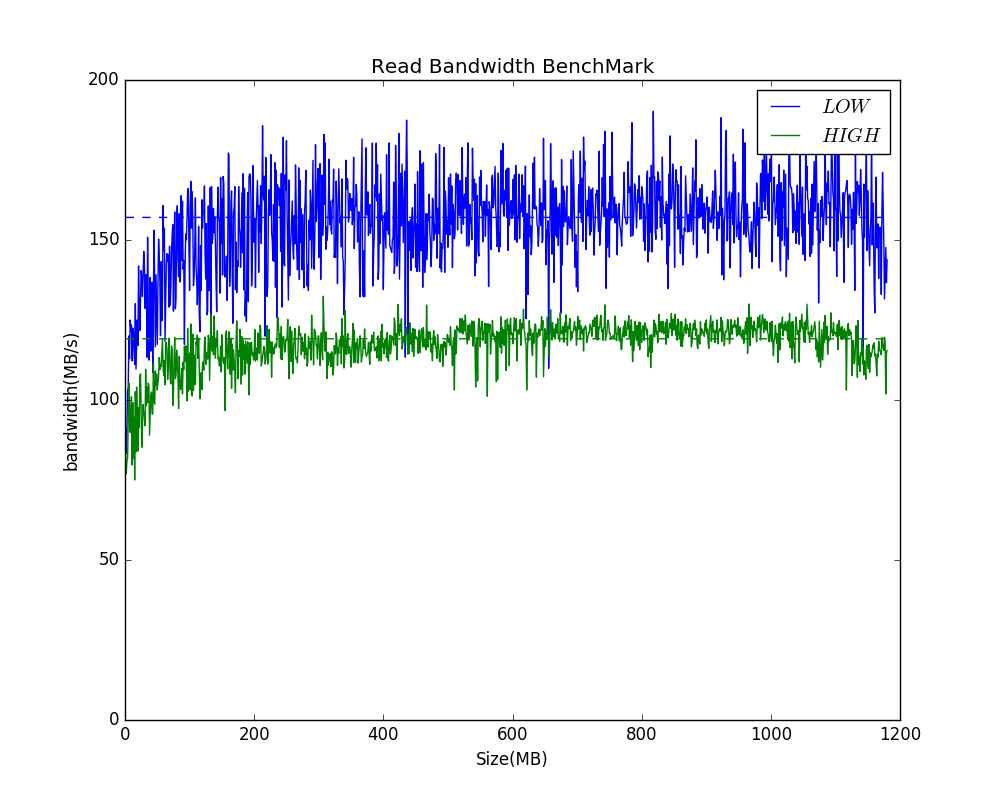
\includegraphics[width=1\textwidth,height=2.8in]{Pics/figure_bw_r.png}
	\caption{数据读取带宽}
	\label{fig:21}
\end{figure}
仿真系统处理数据写入时,首先将原始数据块按照预定义的数据大小分成一个个数据单元,根据系统的缓存参数和目标文件的大小来决定缓存的数据单元数量,并开始针对每个数据单元完成冗余加密操作,后端将缓存的加密数据单元按照次序写入阵列中存储,写入带宽衡量的是这整个过程中原始文件完成冗余加密存储的处理带宽。写入带宽测试结果如\autoref{fig:22}所示。
\begin{figure}[H]
	\centering
	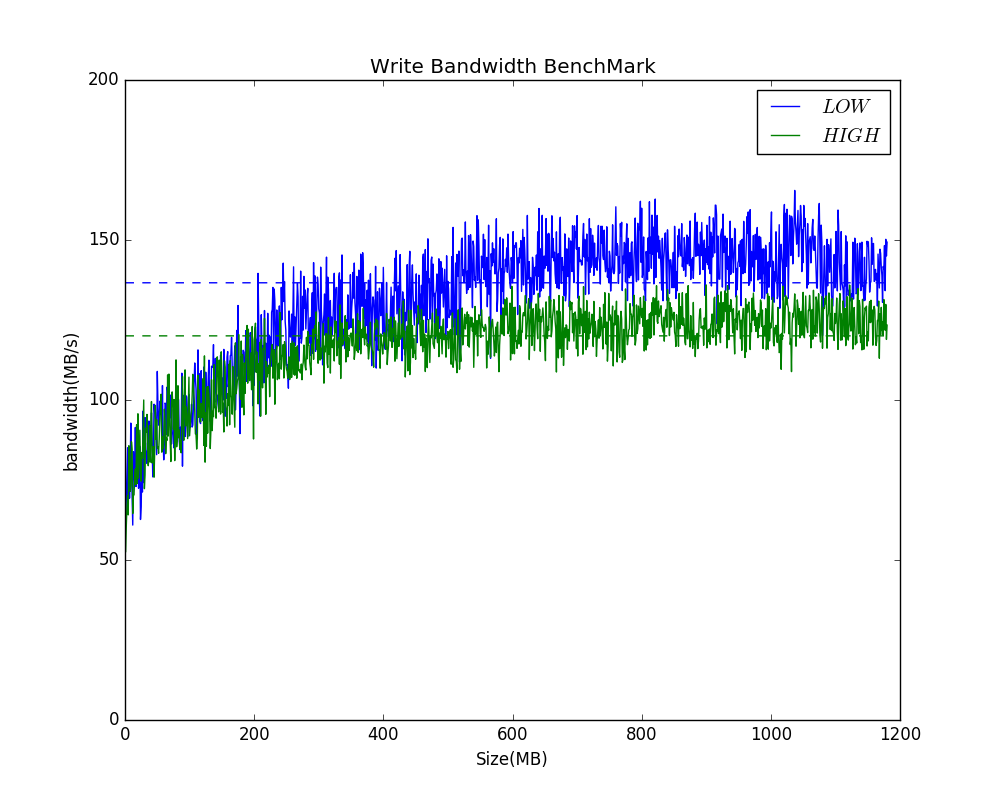
\includegraphics[width=1\textwidth,height=2.8in]{Pics/figure_bw_w.png}
	\caption{数据写入带宽}
	\label{fig:22}
\end{figure}


从读写带宽的测试结果可以看出,在一般加密级别下,数据读取带宽平均水平在158MB/s左右,而数据写入带宽大约为130MB/s。在高强度加密级别下,数据读写带宽整体都比一般加密级别要低一些,其中读取带宽大约是129MB/s,而写入带宽也是在120MB/s左右。


整体上,高强度加密级别的数据处理带宽比一般级别的要低,是因为数据单元在经过非对称加密的过程所耗费的时间要长,但是这种情况是在原始数据量大的情况下,此时加密模块的操作耗费时间成为仿真系统的主要瓶颈。在数据量较小时,二者的差别主要在数据预取和数据缓存的不同上,差别不是很大。


用于存储的SSD盘规格是读取速度为180MB/s,写入速度133MB/s。与原始盘的读写速度相比,仿真系统在写入状态下基本已经达到峰值,而读取状态的损失大约分别在12.2\%和33.3\%,考虑到日常使用对固态盘的损耗,方案的读取性能是可以接受的。


另外,仿真系统的读写带宽最终都稳定在平均水平附近,波动很小,可以得出,系统在处理数据带宽方面,具有一定的稳定性。
\section{I/O时延测试}
I/O延迟测试,在数据被读取时,是计量从发出请求,到缓存模块将第一个数据单元对应的加密数据单元全部取出,推送到解密模块处理的时间。读取时间延迟测试结果如\autoref{fig:23}所示。
\begin{figure}[H]
	\centering
	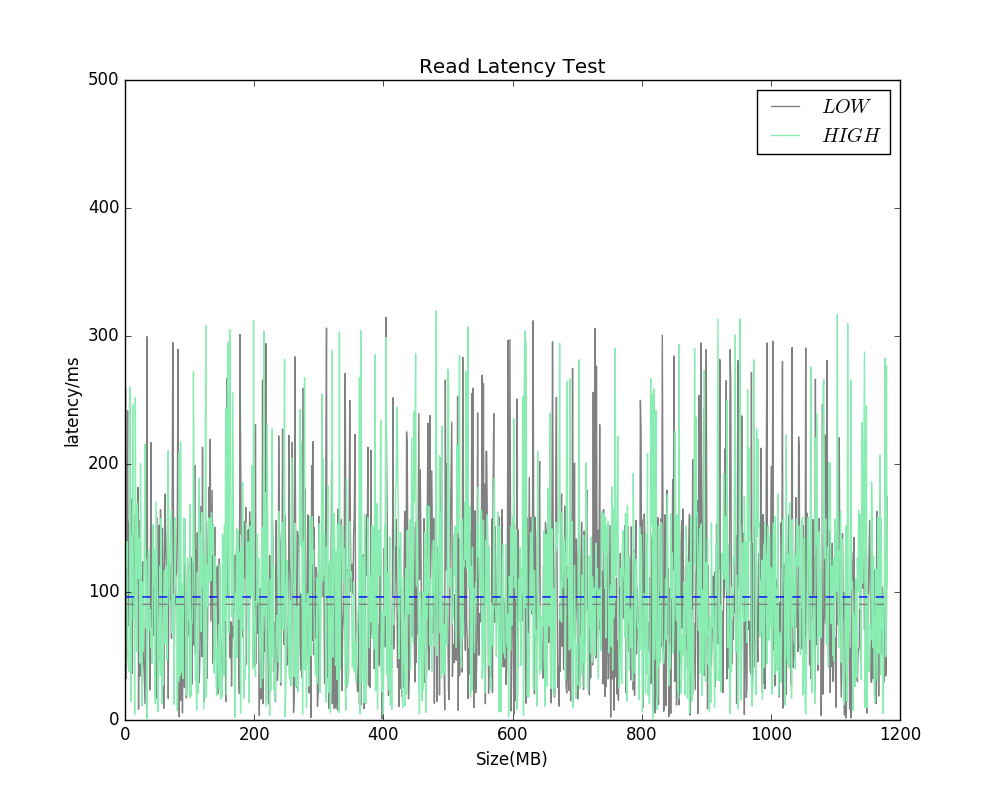
\includegraphics[width=1\textwidth,height=2.8in]{Pics/figure_lat_r.png}
	\caption{系统读取延迟}
	\label{fig:23}
\end{figure}
在写入数据时,是记录第一个数据单元推送到加密模块的时间。写入时间延迟测试结果如\autoref{fig:24}所示。
\begin{figure}[H]
	\centering
	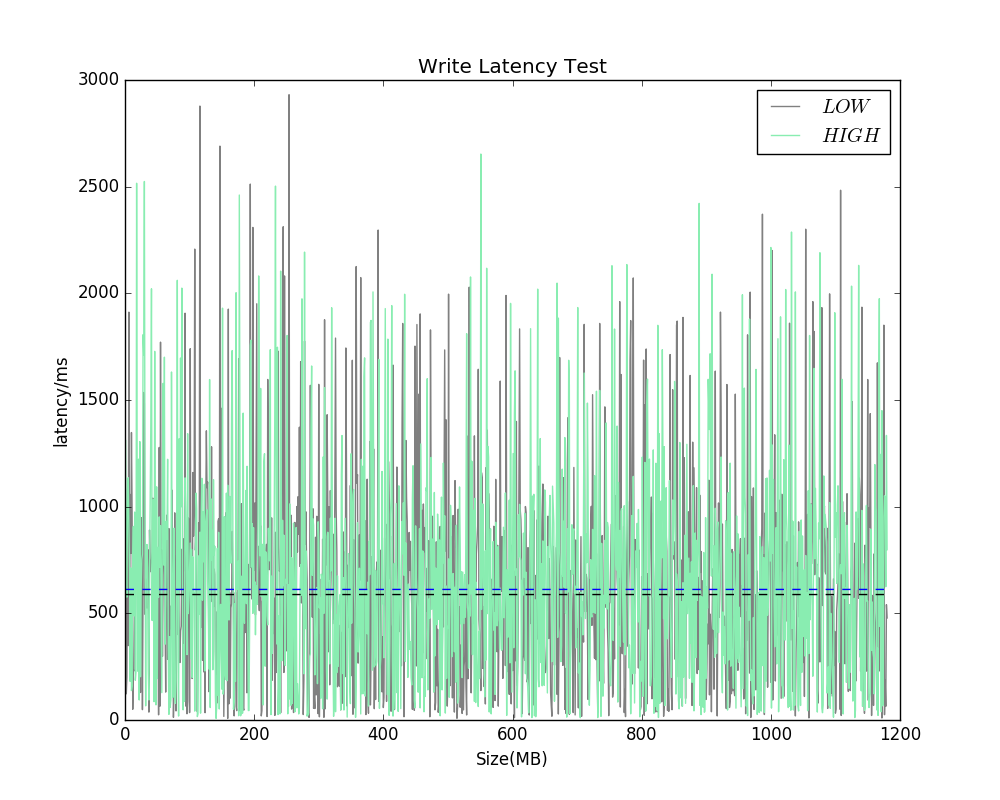
\includegraphics[width=1\textwidth,height=2.8in]{Pics/figure_lat_w.png}
	\caption{系统写入延迟}
	\label{fig:24}
\end{figure}
从时间延迟测试结果来看,仿真系统的读取延迟和写入延迟在不同加密级别下的差别很小,其中读取延迟大约为90ms左右,读取延迟最差不超过300ms。写入延迟均在600ms附近波动,最差情况不超过3000ms。两种测试情形下,系统时延波动都比较显著,然而大部分延迟数据都集中在平均水平,从这点来看,系统的时延也具有一定的稳定性。
\section{系统负载测试}
资源占用测试分为代表仿真系统需要的计算资源和内存资源,系统在对数据进行冗余加密时需要耗费更多的CPU时间片,在缓存读取数据和加密后数据时需要额外的内存空间,因此,从进程的CPU占用和内存占用就可以反映整体系统运行需要的环境。其中前端负载表示的主要是I/O请求、加密这些即时性的负载,后端表示的是数据存储、读取这些长时间的负载。系统不同安全级别下的CPU负载如\autoref{fig:25}和\autoref{fig:26}所示。
\begin{figure}[H]
	\centering
	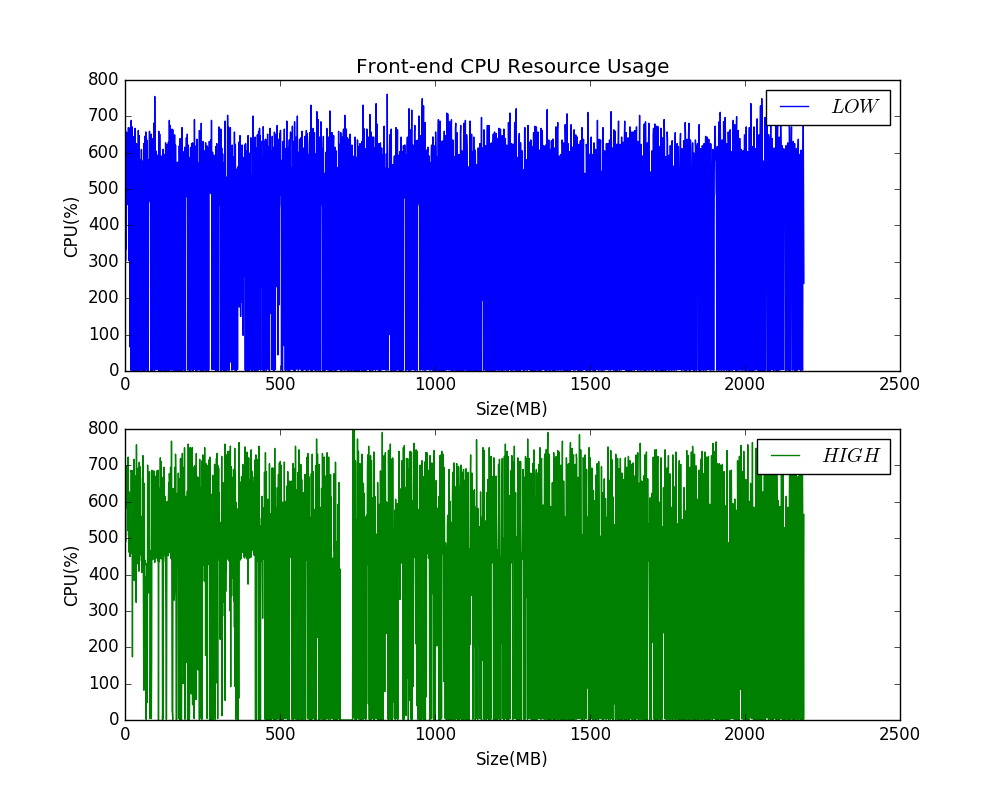
\includegraphics[width=1\textwidth,height=3.5in]{Pics/figure_cpu_client.png}
	\caption{系统前端CPU占用}
	\label{fig:25}
\end{figure}
\begin{figure}[H]
	\centering
	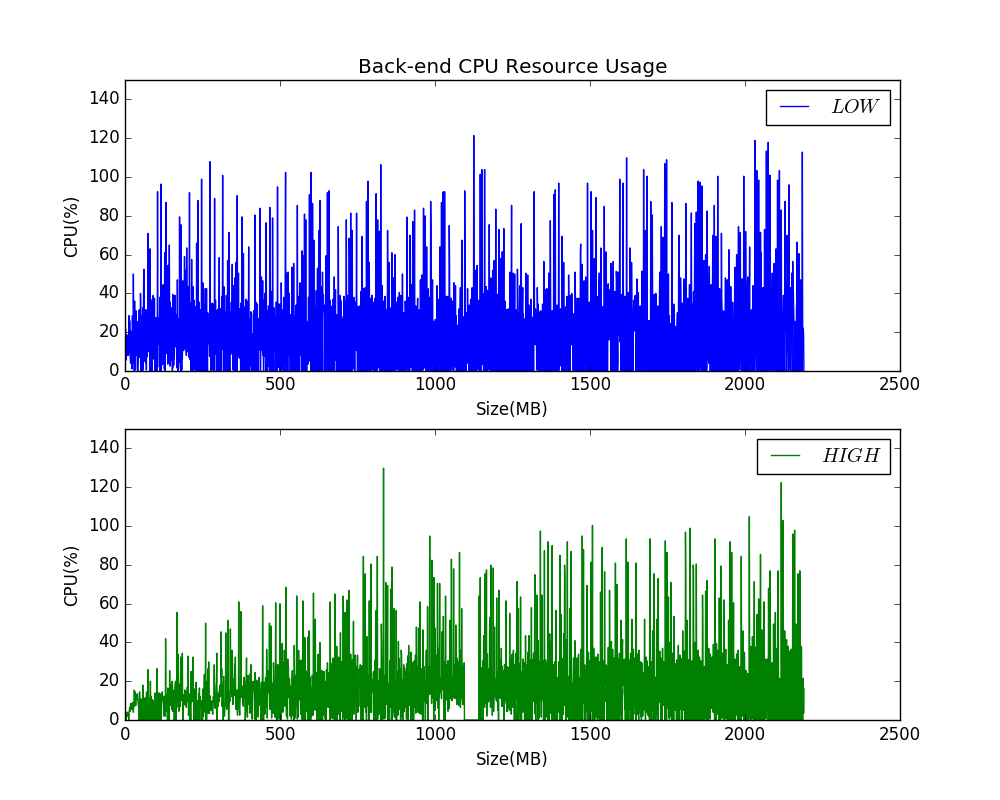
\includegraphics[width=1\textwidth,height=3.5in]{Pics/figure_cpu_server.png}
	\caption{系统后端CPU占用}
	\label{fig:26}
\end{figure}
前后端内存负载分别如\autoref{fig:27}和\autoref{fig:28}所示。
\begin{figure}[H]
	\centering
	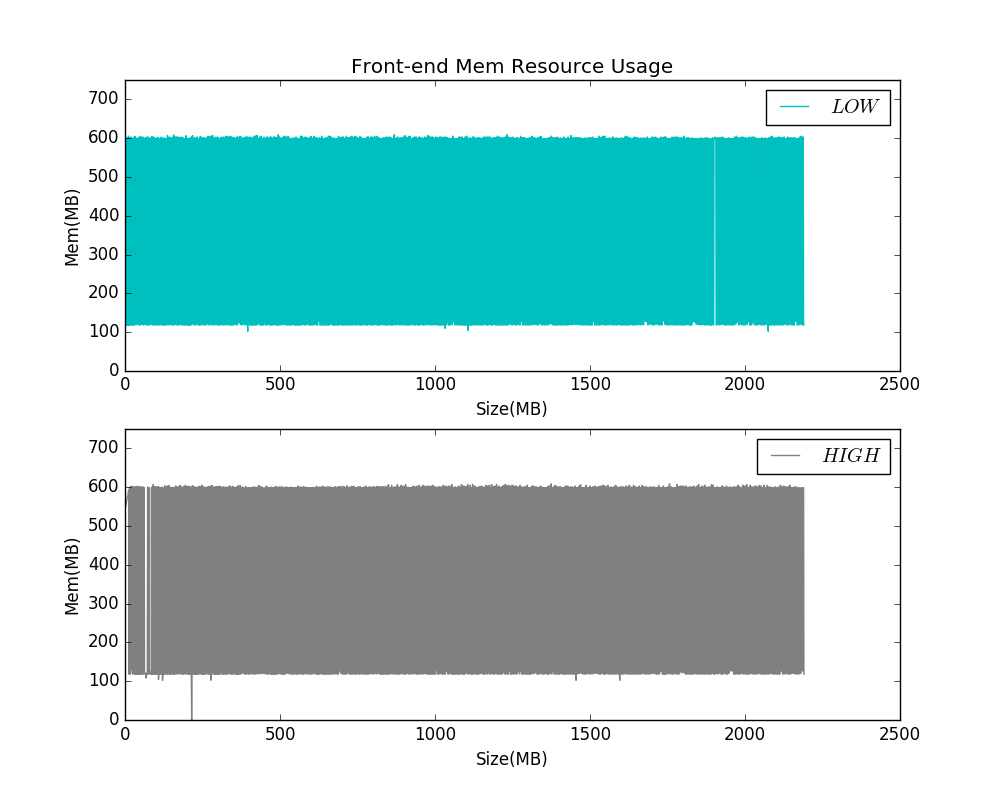
\includegraphics[width=1\textwidth,height=3.5in]{Pics/figure_mem_client.png}
	\caption{系统前端内存占用}
	\label{fig:27}
\end{figure}
\begin{figure}[H]
	\centering
	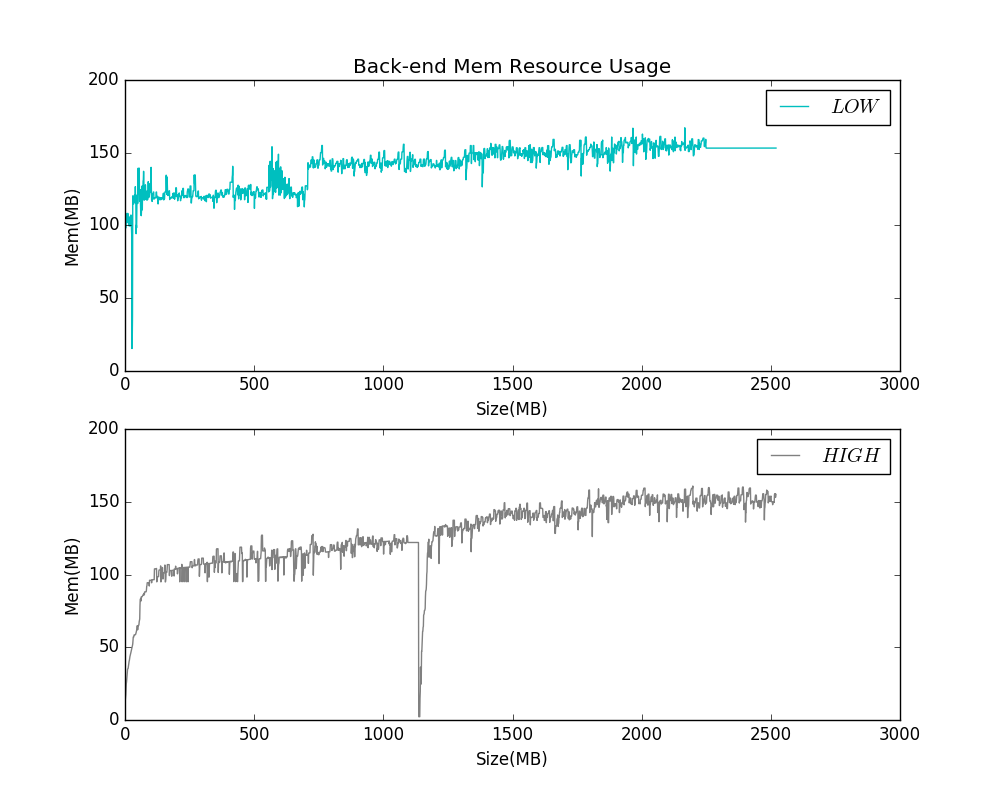
\includegraphics[width=1\textwidth,height=3.5in]{Pics/figure_mem_server.png}
	\caption{系统后端内存占用}
	\label{fig:28}
\end{figure}
从负载测试结果来看,由于前端处理的任务具有瞬时性,加密操作耗费计算资源,所以两种加密级别下的CPU占用都在0到700\%之间变化,内存负载也在100MB到600MB左右变动,可以推断,仿真系统空闲时,前端几乎不占用计算资源,内存占用也在100MB左右。前端总体负载差异较大。


后端处理的任务主要是数据的缓存,读写这些请求,具有长期性的特点,不同的I/O请求对其影响比较平稳,因此测试结果显示的数据趋势比较平缓,其中CPU负载保持在20\%-40\%,内存负载保持在100MB-150MB范围内。后端总体负载比较小且稳定。
\section{数据冗余率测试}
数据冗余表示加密后的数据总量相比原始数据大小的差值,与原始数据的比值,由于系统设计方案是一种冗余存储系统,一个原始数据单元经过处理后,会产生几份冗余的加密数据,因此通过这个比值来判断方案在数据存储层面的可用性,冗余率越低,加密数据占用的存储单元越少,方案的实用性就更好。不同大小的数据冗余率如\autoref{fig:29}所示。
\begin{figure}[H]
	\centering
	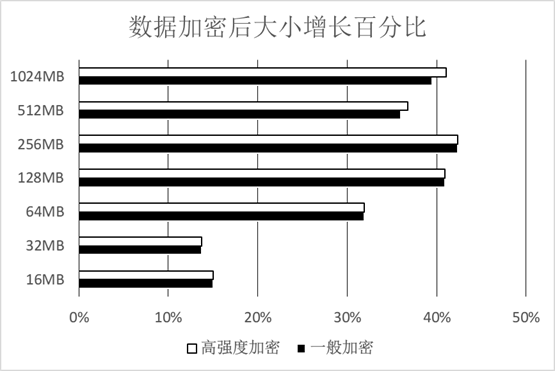
\includegraphics[width=1\textwidth]{Pics/data-ry.png}
	\caption{数据冗余率测试结果}
	\label{fig:29}
\end{figure}
两种强度加密系统,加密后的数据增长率在小文件(<16M)时,基本为0,而在中型文件(16M~64M)时大约为16\%~20\%,在大文件(>64M)时大约在38\%~41\%,不同大小的存储需求,系统的冗余率分为几个区间,在这些区间中变化。


结合上面的一些结论,可以发现,我们的安全删除方案不同安全级别的性能表现确实有差异;而且,整个系统基本可用。由于在物理上删除了元数据,在测试中原始数据无法恢复,系统提示错误。由此得到结论,如果彻底破坏了存储的元数据信息,数据是完全无法恢复的。同时,
在使用本系统中,由于元数据是原始数据块的哈希信息,相比冗余加密后的数据,其对应的元数据大小非常小,存储量不及前者的万分之一。因此,为了保证数据安全删除的效果,
删除元数据信息比删除冗余数据单元,对闪存物理单元的磨损要小很多,达到了本方案提到的减少闪存磨损的优势。


功能测试部分确保了方案的写入、读取、加密、删除功能是可以正常工作并且产生预期效果的,也就是证明了我们方案的有效性。


系统测试分别从带宽、时延、负载、冗余量这四个维度,详细测试了系统的相关性能,根据测试结果的表现并加以分析,初步证明了方案的可行性、可靠性。

\section{本章小结}
本章对全闪存盘阵数据安全删除的仿真系统进行了功能测试和性能测试,测试平台采用的是仿真实验的实现平台,
功能测试部分主要测试了仿真系统的写入、读取、安全删除这些子功能,验证了系统在安全删除关键信息后,数据
无法恢复的方案要求。性能测试部分通过对系统处理带宽、I/O时延、系统负载和冗余率的测试,验证了系统的可行性、可靠性。
同时,安全删除元数据达到数据安全删除的目的,显著降低了闪存物理磨损单元,也就延长了固态盘的使用寿命。

\chapter{总结与展望}
相比目前大量被使用的机械硬盘,固态硬盘由于其读写性能和I/O延迟等优点,
必将成为未来数据存储的主流硬件产品。然而,在阵列领域,由于固态盘的异地
更新可能导致被删除数据泄露的问题,其安全性得不到保障。针对这一问题,
本文在全闪存盘阵的基础上,设计了一种安全删除方案,将原始数据经过冗余加密
后,如果擦除存储的密钥数据,或者擦除一定数量的加密数据,原始数据将再也
无法被还原出来,从而实现了数据的安全存储。本文重点介绍了方案的详细实现,
以及加密流程是如何设计,怎样擦除关键数据保证数据无法恢复,然后,按照方案的设计
思想,实现了一套仿真系统,着重描述了仿真实现中的数据结构设计和相关算法设计,并
结合一系列的测试结果来论证方案的可行性和可靠性。


设计方案和实现仿真实验的过程中,遇到了很多问题。结合这些问题,完成的主要工作如下。
\begin{enumerate}
        \item 调研了固态盘的相关工作机制,由于固态盘的异地更新,原始被删除的数据,可能发生泄露问题。以及
        在TRIM命令在安全删除过程中的作用,TRIM命令和数据多次覆写方法是固态盘安全删除的基础。并了解了相关磁盘
        阵列的存储方式。
        \item 在前人相关的研究基础上,实现并改进了冗余加解密算法,设计了仿真系统中的输入输出缓存数据结构,为了
        实现安全删除功能,将密钥数据单独存储在一个固态盘上。优化了数据处理的流程之后,使得系统整体的性能相比原生
        的读写没有明显的损失,达到了数据安全性和性能的平衡。
        \item 方案针对的环境,不仅针对阵列,而且在iSCSI这些平台上,也能够发挥其作用。只要满足密钥数据存储的固态盘支持
        TRIM命令这一条件,方案就可以在该环境下正常工作,发挥安全删除的作用,具有一定的平台通用性。
\end{enumerate}


目前方案依然存在一些不足之处,由于固态盘阵列的复杂性,没有实现方案对应的原型系统。另外,系统中的密钥数据是存储
在单独的密钥盘上,密钥盘容量通常很小,全盘擦除的代价比较小,在数据安全性和硬件代价上能够得到比较好的平衡。如果
能够将密钥数据存储在盘阵的固定位置,结合阵列的运行机制,实行定点删除,将会使方案的安全性得到极大提升。

%\include{Pics/pic}

%% \include{Pics}

\backmatter

%% 致谢
\begin{ack}
    能完成本研究,首先要感谢我的导师曾令仿老师,是您在忙碌中还对我谆谆教导,细心检查科研过程中的错误。您的每一次指导,都让我学习到了很多东西。感谢谭支鹏老师,在这两年的时间里对我的
关心和帮助,感谢实验室团队里的其他老师和学生,你们为实验室团队辛苦付出着,我们才有这么好的科研环境。感谢刘文国师兄,在我遇到困惑时能够给予我帮助和启发。


    本文受国家自然科学基金项目“面向非易失存储器的一站式存储访问模型及技术研究”(61472153),湖北省自然科学基金项目“基于固态盘和瓦记录磁盘的冷存储系统关键技术研究”(2015CFB192)资助。
\end{ack}

\bibliography{Ref}

%% 附录部分
%% \appendix
%% \begin{publications}
%% \end{publications}

\end{document}
